\documentclass[12pt, a4paper, zihao=-4, openright]{ctexrep}

% 1. 字体设置：中文宋体，西文 Times New Roman
\usepackage{newtxtext} 
%\usepackage[UTF8, fontset=windows]{ctex} 

% 2. 页面设置：A4幅面，常规边距
\usepackage[a4paper, top=2.54cm, bottom=2.54cm, left=2.54cm, right=2.54cm]{geometry}

% 3. 页眉页脚与双线设置
\usepackage{fancyhdr}
%\pagestyle{fancy}
%\fancyhf{} 
%\fancyhead[C]{\leftmark} 
%%\renewcommand{\headrule}{\vspace{-0.4pt}\hrule height 1.5pt width \headwidth \vspace{-1.2pt}\hrule height 0.5pt width \headwidth}
%\fancyfoot[C]{\thepage}       

\usepackage{enumitem}

% 第一套：圆圈序号 ①②③④，最多10条，用于你现在附件
% 【注意】不要用 enumitem 的 \newlist/\setlist 定义它：enumitem 在每个列表开始时会把
%   \value 临时重定义成自己的宏去测量 label 宽度（enumitem.sty 里的 widest 机制），
%   与本 label 中的 \ifcase\value{...} 冲突；编译时每次 \begin{circlist} 都会插入一个 0
%   并报 "Missing number, treated as zero."，PDF 里的序号还会变成 “0circlisti” 之类乱码。
%   这里改用 LaTeX 原生 list：label 在排版每一项时才展开；\usecounter 会让计数器在每次
%   \begin{circlist} 时自动归零，因此每个列表都从 ① 重新开始。
\newcounter{circlist}
\newcommand{\circlistlabel}{%
    \ifcase\value{circlist}\or①\or②\or③\or④\or⑤\or⑥\or⑦\or⑧\or⑨\or⑩\else\arabic{circlist}\fi}
\newenvironment{circlist}%
    {\begin{list}{\circlistlabel}%
        {\usecounter{circlist}%
        \setlength{\leftmargin}{2em}%
        \setlength{\labelwidth}{1.2em}%
        \setlength{\labelsep}{0.8em}%
        \setlength{\itemsep}{0pt}%
        \setlength{\parsep}{0pt}%
        \setlength{\partopsep}{0pt}%
        \setlength{\topsep}{0.4em}%
        \setlength{\listparindent}{0pt}}}%
    {\end{list}}

% 第二套：括号序号 (1)(2)(3)，无限条，留给后面用
\newlist{paralist}{enumerate}{1}
\setlist[paralist]{
    label=(\arabic*),
    leftmargin=2em,
    itemsep=0pt
}



% 3. 设置常规的 fancy 样式
\pagestyle{fancy}
\fancyhf{} % 清除默认设置
\fancyhead[C]{\leftmark} % 居中显示章标题
\fancyfoot[C]{\thepage} % 居中显示页码

% 自定义双线页眉
\renewcommand{\headrule}{%
	\vspace{-0.4pt}\hrule height 1.5pt width \headwidth 
	\vspace{-1.2pt}\hrule height 0.5pt width \headwidth
}

% 2. 关键步骤：重新定义 plain 样式，使其与 fancy 保持一致
\fancypagestyle{plain}{%
	\fancyhf{} % 清除 plain 样式的默认设置
	\fancyhead[C]{\leftmark} % 让章标题页也显示居中的章标题
	\fancyfoot[C]{\thepage} % 让章标题页也显示居中的页码
	\renewcommand{\headrule}{% % 让章标题页也有双线页眉
		\vspace{-0.4pt}\hrule height 1.5pt width \headwidth 
		\vspace{-1.2pt}\hrule height 0.5pt width \headwidth
	}
}

% 4. 目录超链接与PDF元数据设置
\usepackage{hyperref}
\hypersetup{
    colorlinks=true,          linkcolor=blue,        
    urlcolor=blue,         
    citecolor=green,       
    %bookmarks=true,        
    pdfstartview=FitH      
}

% 5. 章节排版控制
\usepackage{titlesec}
\titleformat{\chapter}[block]{\normalfont\huge\bfseries\centering}{第\,\thechapter\,章}{20pt}{\Huge}
\titlespacing*{\chapter}{0pt}{-10pt}{40pt}
\titleformat{\section}[block]{\normalfont\Large\bfseries\raggedright}{\thesection}{1em}{}

% 6. 其他常用宏包
\usepackage{graphicx}
\usepackage{float}         % 提供 [H]：把图片精确固定在正文位置（不浮动，避免图跑到别的页/别的段落下面）      
\usepackage{booktabs}      
\usepackage{amsmath,amssymb,bm}       
\usepackage{caption}       
\usepackage{setspace}      
\onehalfspacing 

\usepackage{tikz}
\usetikzlibrary{shapes.geometric, arrows.meta,calc} % 几何图形、箭头样式
% 定义节点样式
\tikzstyle{startstop} = [rectangle, rounded corners, minimum width=3cm, minimum height=1cm, text centered, draw=black, fill=white]
\tikzstyle{process}   = [rectangle, minimum width=3cm, minimum height=1cm, text centered, draw=black, fill=white]
\tikzstyle{decision}  = [diamond, aspect=3, minimum width=3cm, minimum height=1.0cm, text centered, draw=black, fill=white]
\tikzstyle{arrow}     = [thick, ->, >=stealth] % 箭头样式

% 7. 目录标题居中
\renewcommand\contentsname{\hfill 目\quad 录 \hfill}

% 8. 【新增】引入 GB/T 7714-2015 参考文献宏包
\usepackage[numbers]{gbt7714}

\usepackage{subfig}  %替代 subfigure，插入子图

\usepackage{multirow}  % 画出有单元合并的表格

\usepackage{footmisc} % 推荐加载此宏包以获得更好脚注效果

\usepackage{tabularx}   % 自适应列宽宏包

\usepackage{siunitx} %用于自定义inch的缩写



% 1. 重命名 \paragraph 为 \subsubsubsection
\newcommand{\subsubsubsection}[1]{\paragraph{#1}\mbox{}\\}

% 2. 设置章节编号深度为3（包含 subsubsubsection）
\setcounter{secnumdepth}{3}

% 3. 设置目录显示深度为3（subsubsubsection 不出现在目录中）
\setcounter{tocdepth}{3}

\newcommand{\inch}{\,\text{''}} %自定义inch的双撇

\newcolumntype{C}{>{\centering\arraybackslash}X}



\begin{document}

% === 封面部分 ===
\begin{titlepage}
    \centering 
    \vspace*{4cm} 
    {\Huge \bfseries \textcolor{red}{9-5/8\inch 井筒深度清洁关键技术升级研究及应用} \par} 
    \vspace{2cm} 
    {\Large \textcolor{red}{项目结题报告} \par} 
    \vspace{4cm} 
    {\Large \textcolor{red}{项目负责人：刘维} \par}
    \vspace{1cm}
    {\Large \textcolor{red}{承担单位：中国石油大学（北京）} \par}
    \vspace{1cm}
    {\Large \textcolor{red}{2026年9月16日} \par}
\end{titlepage}

% === 目录部分 ===
\clearpage
\pagenumbering{Roman} 
\tableofcontents

% === 正文部分 ===
\clearpage
\pagenumbering{arabic} 
\setcounter{page}{1}   


% --- 第一章 ---
\chapter{砂砾、铁屑、结垢物、蜡等井筒内的运移及分布规律研究}
	% !TeX root = ../../main.tex

在修井作业过程中，井筒内原有颗粒物及作业过程中新产生的颗粒物会对井筒工况构成显著影响，不仅会导致井下工具工作效率下降，更可能引发卡钻等重大安全事故。影响颗粒在井筒内悬浮状态及运移特性的关键参数包括：颗粒粒径、密度；井眼尺寸、井斜角度；压井液密度、粘度及流速等多重因素。本章基于流体动力学理论和颗粒动力学，针对砂砾、铁屑、结垢物、蜡质等典型颗粒物在井筒内的运移规律开展系统性研究，通过构建EDEM与Fluent耦合仿真模型，定量分析流体参数（流速、粘度）及井筒结构参数（井斜角度）对固相颗粒运移轨迹、沉积速率及空间分布特征的作用机制。

本章仿真方案的具体实施步骤如下：首先，构建颗粒物模型并配置相关参数，基于EDEM平台按实际物理尺寸完成颗粒注入；其次，在Fluent中搭建流体仿真模型，设定流体域边界条件，并同步构建三维井筒、管柱及环空结构模型；随后，建立Fluent与EDEM的双向耦合接口，模拟井筒真实工况下流速、粘度等关键参数对颗粒物运移轨迹、沉积速率及其空间分布特征的影响机制；最后，通过后处理模块进行量化分析，包括颗粒分布统计与动力学参数提取。具体操作流程见图\ref{fig:flowchart}。
    \begin{figure}[htbp]
        \centering
        \begin{tikzpicture}[node distance=2cm] % 节点间距为2cm
            % 1. 流场初始化（起始节点）
            \node (init) [startstop] {流场初始化};
            % 2. 连续相流场计算（处理节点）
            \node (flow) [process, below of=init] {连续相流场计算};
            % 3. 颗粒模型注入（处理节点）
            \node (inject) [process, below of=flow] {颗粒模型注入};
            % 4. 颗粒时间步长计算（处理节点）
            \node (time1) [process, below of=inject] {颗粒时间步长计算};
            % 5. 颗粒时间步长计算（重复节点，保持流程一致性）
            \node (time2) [process, below of=time1] {颗粒时间步长计算};
            % 6. 颗粒轨迹计算（处理节点）
            \node (trajectory) [process, below of=time2] {颗粒轨迹计算};
            % 7. 更新连续相源项（处理节点）
            \node (update) [process, below of=trajectory] {更新连续相源项};
            % 8. 判断是否收敛（决策节点）
            \node (converge) [decision, below of=update] {是否收敛};
            % 9. 判断是否计算完成（决策节点）
            \node (complete) [decision, below of=converge] {是否计算完成};
            % 10. 计算结果（终止节点）
            \node (result) [startstop, below of=complete] {计算结果};
            % 11. 更新下一步时间数据（右侧辅助节点）
            \node (nextstep) [process, right of=complete, xshift=4cm] {更新下一步时间数据};

            % 绘制箭头连线
            \draw [arrow] (init) -- (flow);                          % 流场初始化 → 连续相流场计算
            \draw [arrow] (flow) -- (inject);                        % 连续相流场计算 → 颗粒模型注入
            \draw [arrow] (inject) -- (time1);                       % 颗粒模型注入 → 颗粒时间步长计算
            \draw [arrow] (time1) -- (time2);                        % 颗粒时间步长计算 → 颗粒时间步长计算
            \draw [arrow] (time2) -- (trajectory);                   % 颗粒时间步长计算 → 颗粒轨迹计算
            \draw [arrow] (trajectory) -- (update);                  % 颗粒轨迹计算 → 更新连续相源项
            \draw [arrow] (update) -- (converge);                    % 更新连续相源项 → 判断是否收敛

            % 收敛判断分支（未收敛→返回连续相流场计算）
            \draw [arrow] (converge.west) -- ++(-1,0) |- (flow.west) node[midway, left] {否};

            % 收敛后→计算完成判断
            \draw [arrow] (converge) -- (complete);

            % 计算完成判断分支（未完成→更新下一步时间数据→返回连续相流场计算）
            \draw [arrow] (complete.east) -- (nextstep.west) node[midway, above] {否};
            \draw [arrow] (nextstep.north) |- (flow.east);

            % 计算完成→输出结果
            \draw [arrow] (complete) -- (result) node[midway, right] {是};

        \end{tikzpicture}
        \caption{颗粒运移模型计算流程图}
        \label{fig:flowchart}  
    \end{figure}

\section{基本理论和模拟条件}  
\subsection{EDEM理论基础} 
井筒中的颗粒在运动过程中相互接触和碰撞是不可避免的，颗粒间出现接触时将产生作用力。EDEM软件的理论基础是离散元法，离散单元法的基础模型是颗粒之间的相互接触，分析过程中颗粒所受外力作用以及力矩都是通过接触模型直接决定的。在进行离散元分析时根据分析工况将离散颗粒相接触模型分为干颗粒和湿颗粒两种类型。
当计算物料为干颗粒时，颗粒与其余接触点之间不存在粘结的作用，此时接触模型即可选择EDEM软件中的Hertz-Mindlin基本接触模型，该模型也是EDEM软件中默认选择的颗粒接触模型。建立如图\ref{fig:particle_collision}所示的颗粒碰撞受力模型，并分析颗粒间力的传递。

    \begin{figure}[htbp]
    \centering
    % 双颗粒碰撞模型示意图：改用外部图片（原 TikZ 手绘图见 git 历史）
    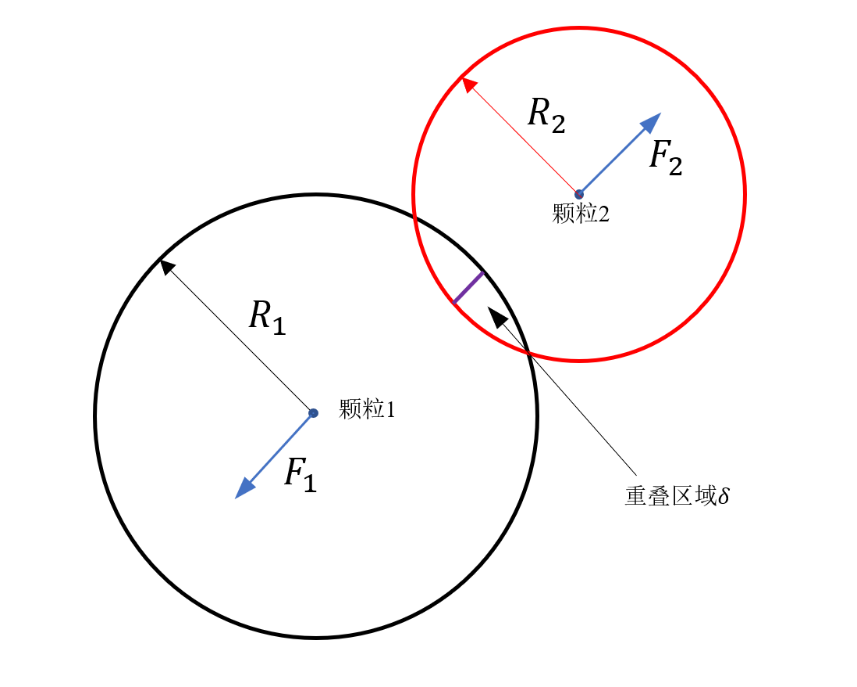
\includegraphics[width=8cm]{figure/kelipengzhuang.png}
    \caption{双颗粒碰撞模型示意图}
    \label{fig:particle_collision}
\end{figure}


假设发生弹性接触的两球形颗粒的半径分别为 \(R_{1}\)、\(R_{2}\)，则颗粒间产生的法向接触力大小 \(F_{\mathrm{n}}\) 的计算式为
\begin{equation}
	F_{\mathrm{n}}=\frac{4}{3}E_{\mathrm{eq}}\sqrt{R_{\mathrm{eq}}}\,\alpha^{3/2}
\end{equation}
式中，\(E_{\mathrm{eq}}\) 为等效杨氏模量，GPa；\(\alpha\) 为法向重叠量，mm；\(R_{\mathrm{eq}}\) 为等效接触半径。

\(R_{\mathrm{eq}}\) 的计算式为
\begin{equation}
	R_{\mathrm{eq}}=\frac{R_{1}R_{2}}{R_{1}+R_{2}}
\end{equation}

颗粒间法向阻尼力 \(F_{\mathrm{n}}^{\mathrm{d}}\) 以及切向阻尼力 \(F_{\mathrm{t}}^{\mathrm{d}}\) 的计算公式为
\begin{equation}
	F_{\mathrm{n}}^{\mathrm{d}}=-2\sqrt{\frac{5}{6}}\beta\sqrt{S_{\mathrm{n}}m_{\mathrm{eq}}}\,\nu_{\mathrm{n}}^{\mathrm{rel}}
\end{equation}
\begin{equation}
	F_{\mathrm{t}}^{\mathrm{d}}=-2\sqrt{\frac{5}{6}}\beta\sqrt{S_{\mathrm{t}}m_{\mathrm{eq}}}\,\nu_{\mathrm{t}}^{\mathrm{rel}}
\end{equation}
式中，\(S_{\mathrm{t}}\) 为切向刚度，N/m；\(S_{\mathrm{n}}\) 为法向刚度，N/m；\(\nu_{\mathrm{t}}^{\mathrm{rel}}\) 为切向真实速度，m/s；\(\nu_{\mathrm{n}}^{\mathrm{rel}}\) 为法向真实速度，m/s；\(e\) 为恢复系数；\(m_{\mathrm{eq}}\) 为等效质量，kg。

其中，\(G_{\mathrm{eq}}\) 为等效剪切模量，Pa，其计算公式为
\begin{equation}
	G_{\mathrm{eq}}=\left(\frac{2-\nu_{1}}{G_{1}}+\frac{2-\nu_{2}}{G_{2}}\right)^{-1}
\end{equation}
式中，\(G_{1}\)、\(G_{2}\) 分别为球 1、2 的剪切模量；\(\nu_{1}\)、\(\nu_{2}\) 分别为颗粒 1、2 的泊松比。

假设两颗粒产生接触前的速度分别为 \(\bm{\nu}_{1}\)、\(\bm{\nu}_{2}\)，\(\bm{n}\) 为产生接触时的法向单位矢量，则
\begin{equation}
	\bm{n}=\frac{\bm{r}_{1}-\bm{r}_{2}}{\left|\bm{r}_{1}-\bm{r}_{2}\right|}
\end{equation}
\begin{equation}
	\nu_{\mathrm{n}}^{\mathrm{rel}}=(\bm{\nu}_{1}-\bm{\nu}_{2})\cdot\bm{n}
\end{equation}

颗粒间的切向力 \(F_{\mathrm{t}}\) 计算式为
\begin{equation}
	F_{\mathrm{t}}=S_{\mathrm{t}}\delta
\end{equation}

摩擦力 \(\mu_{\mathrm{s}}F_{\mathrm{n}}\) 与切向力的大小有关，\(\mu_{\mathrm{s}}\) 为静摩擦系数。滚动摩擦在仿真计算过程中的重要性是不言而喻的，接触表面处产生的力矩可以对动摩擦系数进行描述，即
\begin{equation}
	\bm{T}_{\mathrm{t}}=\mu F_{\mathrm{n}}R\,\bm{\omega}_{\mathrm{t}}
\end{equation}
式中，\(\mu\) 为动摩擦系数；\(R\) 为接触点到质心的长度，mm；\(\bm{\omega}_{\mathrm{t}}\) 为物体到接触点的单位角速度，rad/s。

当处理颗粒为湿颗粒且存在粘性作用时，需要模拟含湿颗粒且颗粒间能形成液桥力的工况，接触模型通常选择为 Hertz--Mindlin with JKR 接触模型，模型接触力的实现基于 Johnson--Kendall--Roberts 理论。该模型的计算基础与 Hertz--Mindlin 基本接触模型相同，是在 Hertz--Mindlin 接触模型基础上引入一个法向接触力。

JKR 模型的法向力由重叠量 \(\delta\) 和引入的新参数表面能 \(\gamma\) 实现：
\begin{equation}
	F_{\mathrm{JKR}}
	=-4\sqrt{\pi\gamma E_{\mathrm{eq}}\alpha^{3}}
	+\frac{4E_{\mathrm{eq}}\alpha^{3}}{3R_{\mathrm{eq}}}
\end{equation}
\begin{equation}
	\delta=\frac{\alpha^{2}}{R_{\mathrm{eq}}}
	-\sqrt{\frac{4\pi\gamma\alpha}{E_{\mathrm{eq}}}}
\end{equation}

对于 \(\gamma=0\) 的情况，接触力即变为 Hertz--Mindlin 法向力：
\begin{equation}
	F_{\mathrm{JKR}}=F_{\mathrm{Hertz}}
	=\frac{4}{3}E_{\mathrm{eq}}\sqrt{R_{\mathrm{eq}}}\,\alpha^{3/2}
\end{equation}

计算时可根据计算工况调整颗粒表面能及其他参数，调整不同含水率条件下的颗粒状态，不同工况的表面能对颗粒影响较大。该接触模型对颗粒提供凝聚力，即使颗粒间的接触不是直接接触也会存在。颗粒间有非零凝聚力的最大间隙计算式为
\begin{equation}
	\delta_{\mathrm{c}}
	=\frac{\alpha_{\mathrm{c}}^{2}}{R_{\mathrm{eq}}}
	-\sqrt{\frac{4\pi\gamma\alpha_{\mathrm{c}}}{E_{\mathrm{eq}}}}
\end{equation}

当 \(\delta<\delta_{\mathrm{c}}\) 时，模型计算则计算为 0。当颗粒间的凝聚力达到最大值时，颗粒间的接触不是实际接触，而且接触间隔小于 \(\delta_{\mathrm{c}}\)，其计算式为
\begin{equation}
	F_{\mathrm{c}}=-\frac{3}{2}\pi\gamma R_{\mathrm{eq}}
\end{equation}

颗粒与颗粒间接触模型是 EDEM 中使用的 Hertz--Mindlin 默认模型，该模型适用于描述各种形状颗粒之间的接触行为，包括圆形、椭圆形和不规则形状颗粒，如图 1.3、图 1.4 所示。Hertz--Mindlin 模型在描述颗粒间接触力和相互作用时具有广泛的适用性，并且考虑了颗粒的变形和滑移等实际因素。Hertz--Mindlin 接触模型示意图见图 1.3。

此外，在采用 EDEM 软件进行模拟计算过程中，还需要做如下假设：
\begin{enumerate}
	\item 颗粒系统中所有颗粒的点变形总和被认为是颗粒系统的总变形；
	\item 颗粒之间的接触形式为点接触，接触总是在很小的区域内发生；
	\item 颗粒与颗粒接触时可以产生部分重叠量，但重叠量大小与颗粒尺寸大小相比要小很多；
	\item 在每个计算步长内，外界激励不能被任意颗粒同时传播到它的相邻颗粒。在所有的计算时间内，任意颗粒上的合力可以通过相互接触的颗粒之间的相互作用唯一确定。
\end{enumerate}

\begin{figure}[htbp]
	\centering
	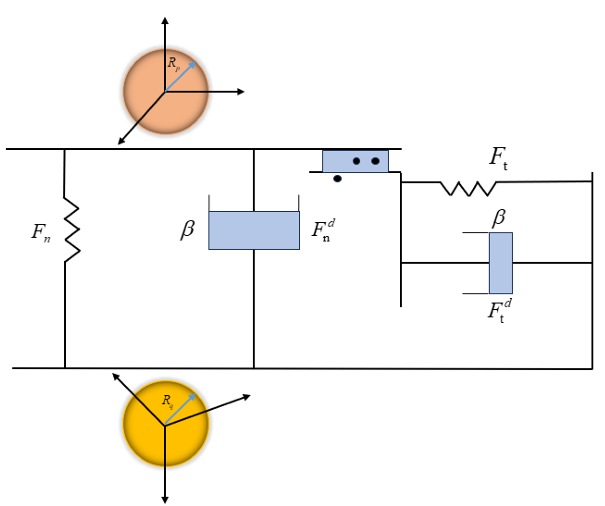
\includegraphics[width=0.6\textwidth]{figure/hertz-mindlin-contact-model.png}
	\caption{Hertz--Mindlin 接触模式示意图}
	\label{fig:hertz_mindlin_contact_model}
\end{figure}

\begin{figure}[htbp]
	\centering
	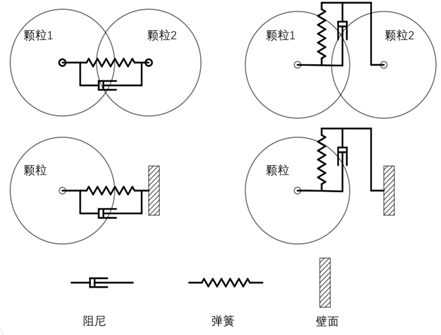
\includegraphics[width=0.6\textwidth]{figure/hertzian-soft-sphere-model.png}
	\caption{Hertzian 软球模型}
	\label{fig:hertzian_soft_sphere_model}
\end{figure}

\subsection{液固相间作用模型}

颗粒在流场中的受力主要分为以下三类：
\begin{enumerate}
	\item 与流体--颗粒相对运动无关的力，包括重力、压力梯度力、浮力等；
	\item 与流体--颗粒相对运动有关，且力的方向沿相对运动方向，包括曳力、虚拟质量力和 Basset 力等；
	\item 与流体--颗粒相对运动有关，且力的方向垂直于相对运动方向，包括 Saffman 力、Magnus 力等。
\end{enumerate}

在液--固两相流的模拟中，正确选择曳力模型有助于提高数值模拟的准确性。常见曳力模型有 Schiller--Naumann 曳力模型、Wen--Yu 曳力模型、Symmetric 曳力模型、Gidaspow 曳力模型、Syamlal--O'Brien 曳力模型等。Gidaspow 曳力模型应用较广，适用于大多数流态化计算，是 Wen--Yu 曳力模型与 Ergun 曳力模型的结合。因此，本文研究主要采用 Gidaspow 曳力模型，如下式所示：
\begin{equation}
	\beta_{\mathrm{Gidaspow}}=
	\begin{cases}
		\dfrac{3C_{\mathrm{d}}\epsilon_{\mathrm{s}}\rho_{\mathrm{l}}\left|\bm{\nu}_{\mathrm{l}}-\bm{\nu}_{\mathrm{s}}\right|}{4d_{\mathrm{s}}}\epsilon_{\mathrm{l}}^{-2.65}, & \epsilon_{\mathrm{l}}>0.8 \\[10pt]
		\dfrac{\epsilon_{\mathrm{s}}(1-\epsilon_{\mathrm{l}})\mu_{\mathrm{l}}}{\epsilon_{\mathrm{l}}d_{\mathrm{s}}^{2}}
		+1.75\dfrac{\epsilon_{\mathrm{s}}\rho_{\mathrm{l}}}{d_{\mathrm{s}}}
		\left|\bm{\nu}_{\mathrm{l}}-\bm{\nu}_{\mathrm{s}}\right|, & \epsilon_{\mathrm{l}}\leq 0.8
	\end{cases}
\end{equation}
其中，\(C_{\mathrm{d}}\) 为阻力系数，其计算公式如下：
\begin{equation}
	C_{\mathrm{d}}=
	\begin{cases}
		\dfrac{24}{Re_{\mathrm{s}}}\left(1+0.15Re_{\mathrm{s}}^{0.687}\right), & Re_{\mathrm{s}}\leq 1000 \\[8pt]
		0.44, & Re_{\mathrm{s}}>1000
	\end{cases}
\end{equation}

固相雷诺数表示为
\begin{equation}
	Re_{\mathrm{s}}=\frac{d_{\mathrm{s}}\epsilon_{\mathrm{l}}\rho_{\mathrm{l}}
		\left|\bm{\nu}_{\mathrm{l}}-\bm{\nu}_{\mathrm{s}}\right|}{\mu_{\mathrm{l}}}
\end{equation}

升力包括剪切升力（Saffman）和旋转升力（Magnus），垂直于颗粒和流体之间的相对速度方向。施加在岩屑颗粒 \(p\) 上的剪切升力（Saffman）表现形式为
\begin{equation}
	\bm{F}_{\mathrm{S}}
	=C_{\mathrm{LS}}\frac{\rho_{\mathrm{l}}\pi}{8}d_{p}^{3}
	\left|\bm{\nu}_{\mathrm{l}}-\bm{\nu}_{p}\right|
	\sqrt{\omega_{\mathrm{l}}}
\end{equation}
其中，\(\omega_{\mathrm{l}}\) 为流体速度的旋度，\(C_{\mathrm{LS}}\) 为剪切升力系数，可以表示为
\begin{equation}
	C_{\mathrm{LS}}=\frac{4.1126}{Re_{\mathrm{s}}^{0.5}}f\left(Re_{\mathrm{HB}},Re_{\mathrm{s}}\right)
\end{equation}
\begin{equation}
	f\left(Re_{\mathrm{HB}},Re_{\mathrm{s}}\right)
	=
	\begin{cases}
		\left(1-0.3314\sqrt{\beta}\right)
		e^{-0.1Re_{\mathrm{s}}}
		+0.3314\sqrt{\beta}, & Re_{\mathrm{s}}\leq 40 \\[6pt]
		0.0524\sqrt{\beta Re_{\mathrm{s}}}, & Re_{\mathrm{s}}>40
	\end{cases}
\end{equation}
其中
\begin{equation}
	\beta=\frac{0.5Re_{\mathrm{s}}}{Re_{\mathrm{HB}}},\qquad 0.005<\beta<0.4
\end{equation}

剪切流的雷诺数为
\begin{equation}
	Re_{\mathrm{s}}=\frac{\rho_{\mathrm{l}}d_{p}^{2}\omega_{\mathrm{l}}}{\mu_{\mathrm{l}}}
\end{equation}

作用在颗粒 \(p\) 上的旋转升力（Magnus）的计算公式由 Oesterle 给出：
\begin{equation}
	\bm{F}_{\mathrm{M}}
	=C_{\mathrm{LM}}\frac{\rho_{\mathrm{l}}\pi}{8}d_{p}^{3}
	\left|\bm{\nu}_{\mathrm{l}}-\bm{\nu}_{p}\right|
	\frac{\left|\bm{\Omega}\times
		\left(\bm{\nu}_{\mathrm{l}}-\bm{\nu}_{p}\right)\right|}
	{\left|\bm{\Omega}\right|}
\end{equation}
其中，\(C_{\mathrm{LM}}\) 为剪切升力系数，可以表示为：
\begin{equation}
	C_{\mathrm{LM}}
	=0.45+\left(\frac{Re_{r}}{Re_{\mathrm{HB}}}-0.454\right)
	\exp\left(-0.5684Re_{r}Re_{\mathrm{HB}}^{-0.3}\right)
\end{equation}

颗粒拟温度的物理意义表示颗粒脉动的脉动能，能够在微尺度上反映颗粒脉动速度的剧烈程度，表征颗粒运动的无序程度，是颗粒相相互碰撞作用以及颗粒相和流体相相互作用的结果。颗粒拟温度的定义为
\begin{equation}
	\theta=\frac{1}{3N}\left[
	\sum_{j=1}^{N}C_{xj}^{2}
	+\sum_{j=1}^{N}C_{yj}^{2}
	+\sum_{j=1}^{N}C_{zj}^{2}
	\right]
\end{equation}

\subsection{液相控制模型}

对于密度恒定的不可压缩流体，假设液相质量为常数，液体流动遵循 N--S 方程。液固两相流模型中流体相的连续性方程和 N--S 方程由下式给出：
\begin{equation}
	\frac{\partial(\rho_{\mathrm{l}}\epsilon_{\mathrm{l}})}{\partial t}
	+\nabla\cdot(\rho_{\mathrm{l}}\epsilon_{\mathrm{l}}\bm{\nu}_{\mathrm{l}})=0
\end{equation}
\begin{equation}
	\frac{\partial(\rho_{\mathrm{l}}\epsilon_{\mathrm{l}}\bm{\nu}_{\mathrm{l}})}{\partial t}
	+\nabla\cdot(\rho_{\mathrm{l}}\epsilon_{\mathrm{l}}\bm{\nu}_{\mathrm{l}}\bm{\nu}_{\mathrm{l}})
	=-\epsilon_{\mathrm{l}}\nabla P
	-\nabla\cdot(\epsilon_{\mathrm{l}}\bm{\tau}_{\mathrm{l}})
	+\epsilon_{\mathrm{l}}\rho_{\mathrm{l}}\bm{g}+\bm{F}_{p}
\end{equation}
式中，\(\bm{g}\) 为重力加速度，\(\rho_{\mathrm{l}}\) 为流体密度，\(P\) 和 \(\epsilon_{\mathrm{l}}\) 分别为流体相压力和体积分数，\(\bm{\nu}_{\mathrm{l}}\) 为流体速度，\(\bm{F}_{p}\) 为液固相间作用力，\(\bm{\tau}_{\mathrm{l}}\) 表示粘性应力张量。其中，液固相间作用力及粘性应力张量公式为
\begin{equation}
	\bm{F}_{p}
	=-\frac{\sum_{i=1}^{k_{\mathrm{c}}}\bm{F}_{i,p}}{\Delta V}
\end{equation}
\begin{equation}
	\bm{\tau}_{\mathrm{l}}
	=\mu_{\mathrm{l}}\left[
	\nabla\bm{\nu}_{\mathrm{l}}
	+\left(\nabla\bm{\nu}_{\mathrm{l}}\right)^{T}
	\right]
	-\frac{2}{3}\mu_{\mathrm{l}}
	\left(\nabla\cdot\bm{\nu}_{\mathrm{l}}\right)\bm{I}
\end{equation}
式中，\(\bm{F}_{p}\) 为液体对颗粒 \(p\) 的作用力，\(\mu_{\mathrm{l}}\) 为流体粘度，\(\bm{I}\) 为单位二阶张量。

\subsection{湍流模型}

考虑到高精度、应用简单、计算效率和通用性等需求，本文采用 \(k-\epsilon\) 标准模型作为研究基础来计算钻井液的湍流黏度，其中 \(k\) 为湍流动能，\(\epsilon\) 为耗散率。\(k\) 和 \(\epsilon\) 的输运方程分别表示为：
\begin{equation}
	\frac{\partial}{\partial t}(\rho_{\mathrm{l}}k)
	+\frac{\partial}{\partial x_{i}}(\rho_{\mathrm{l}}k\nu_{\mathrm{l},i})
	=\frac{\partial}{\partial x_{j}}\left[
	\left(\mu+\frac{\mu_{\mathrm{t}}}{\sigma_{k}}\right)
	\frac{\partial k}{\partial x_{j}}
	\right]
	+G_{k}-\rho_{\mathrm{l}}\epsilon-Y_{\mathrm{M}}
\end{equation}
\begin{equation}
	\frac{\partial}{\partial t}(\rho_{\mathrm{l}}\epsilon)
	+\frac{\partial}{\partial x_{i}}(\rho_{\mathrm{l}}\epsilon\nu_{\mathrm{l},i})
	=\frac{\partial}{\partial x_{j}}\left[
	\left(\mu+\frac{\mu_{\mathrm{t}}}{\sigma_{\epsilon}}\right)
	\frac{\partial\epsilon}{\partial x_{j}}
	\right]
	+C_{1\epsilon}\frac{\epsilon}{k}
	\left(G_{k}+C_{3\epsilon}G_{b}\right)
	-C_{2\epsilon}\rho_{\mathrm{l}}\frac{\epsilon^{2}}{k}
\end{equation}
式中，\(\rho_{\mathrm{l}}\) 为液相密度，kg/m\(^{3}\)；\(\nu_{\mathrm{l}}\) 为液相速度，m/s；\(C_{1\epsilon}\)、\(C_{2\epsilon}\)、\(C_{3\epsilon}\) 为常数，且 \(C_{1\epsilon}=1.44\)，\(C_{2\epsilon}=1.92\)。\(\sigma_{k}\) 和 \(\sigma_{\epsilon}\) 分别为 \(k\) 和 \(\epsilon\) 的湍流普朗特数，其取值为 \(\sigma_{k}=1.0\)，\(\sigma_{\epsilon}=1.3\)。\(G_{k}\) 表示由于平均速度梯度产生的湍流动能；\(Y_{\mathrm{M}}\) 表示可压缩湍流脉动膨胀对整体耗散率的影响；\(\mu_{\mathrm{t}}\) 表示湍流黏度系数。\(G_{k}\)、\(Y_{\mathrm{M}}\)、\(\mu_{\mathrm{t}}\) 公式表示如下：
\begin{equation}
	Y_{\mathrm{M}}=2\rho_{\mathrm{l}}\epsilon M^{2}
\end{equation}
\begin{equation}
	\mu_{\mathrm{t}}=\frac{\rho_{\mathrm{l}}C_{\mu}k^{2}}{\epsilon}
\end{equation}

为了模拟井筒内携带颗粒的特性，模型需要通过设计一个环形空间来实现。研究中建立了内径 \(\phi 88.9\) mm、外径 \(\phi 244.475\) mm、\(\phi 177.8\) mm、总长度为 \(1.5\) m 的光滑管柱，用于模拟钻杆（\(3\)-\(1/2'\)）和井筒（\(9\)-\(5/8'\)、\(7'\)），套管和钻杆同心。在模拟过程中，内部钻杆固定，钻井液以一定速度垂直于入口方向流入环形空间，并从另一端出口流出。环空模型如图 1.5、图 1.6 所示。在 EDEM 软件中，颗粒产生于“颗粒工厂”，其初始速度、角速度为零，角度随机。计算采用了非稳态 \(k-\epsilon\) 湍流模型，将颗粒设置为离散相，并利用多面体网格进行建模。边界条件包括速度入口、压力出口，管壁采用无滑移条件。一般计算参数具体数值见表 1.1，重力方向始终竖直向下，对于不同 \(\theta\) 的情况，流体域旋转相应角度。

\begin{figure}[htbp]
	\centering
	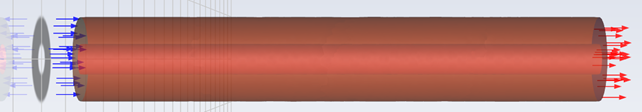
\includegraphics[width=0.9\textwidth]{figure/fluid-domain-geometry.png}
	\caption{流体域几何模型示意图}
	\label{fig:fluid_domain_geometry}
\end{figure}

\begin{figure}[htbp]
	\centering
	
\includegraphics[width=0.9\textwidth]{figure/fluid-domain-polyhedral-mesh.jpg}
	\caption{流体域多面体单元离散示意图}
	\label{fig:fluid_domain_mesh}
\end{figure}

\begin{table}[H]
	\centering
	\caption{一般计算参数}
	\begin{tabular}{llll}
		\toprule
		名称 & 符号 & 数值 & 单位 \\
		\midrule
		水平井筒长度 & \(L\) & 1.5 & m \\
		井筒直径 & \(D_{\mathrm{H}}\) & 244.475/177.8 & mm \\
		钻杆直径 & \(D_{\mathrm{P}}\) & 88.9 & mm \\
		颗粒密度 & \(\rho_{\mathrm{P}}\) & -- & kg/m\(^{3}\) \\
		压井液密度 & \(\rho_{\mathrm{l}}\) & -- & kg/m\(^{3}\) \\
		井斜角 & \(\theta\) & 0.0、45.0、90.0 & \(^{\circ}\) \\
		压井液入口流速 & \(\nu_{\mathrm{c}}\) & 0.17、0.27、0.37、0.59 & m/s \\
		压井液粘度 & \(\mu\) & 1.0、1.7 & mPa·s \\
		\bottomrule
	\end{tabular}
\end{table}

在井筒内颗粒物运移特性的研究中，基于对颗粒动力学行为控制作用的大小，选择流体流速 \(\nu_{\mathrm{c}}\)、流体粘度 \(\mu\) 和井斜角 \(\theta\) 作为主要控制变量。首先，流体流速 \(\nu_{\mathrm{c}}\) 是决定颗粒悬浮与输运能力的关键参数，流速直接影响流体的动能和湍流强度，进而调控颗粒的启动阈值、悬浮状态及沉积风险。其次，流体粘度 \(\mu\) 通过改变流体的粘滞阻力，显著影响颗粒的沉降速度及与流体的相互作用，高粘度流体可增强颗粒携带能力，但可能增加流动阻力。最后，井斜角 \(\theta\) 作为几何特征的核心变量，通过改变重力在井筒轴线方向的分量，直接影响颗粒的受力平衡：在斜井或水平井中，重力分量的减弱会加剧颗粒沉降的方位选择性，导致非对称沉积。这三个因素共同构成了颗粒运移的“动力--阻力--几何”三元耦合机制，能够系统表征复杂井筒环境下颗粒迁移的物理本质，为优化携粒效率、预测床层形成提供理论支撑。考虑到颗粒属性的不同会对其运移行为产生显著影响，于是，下文分别研究砂砾、铁屑、结垢物和蜡颗粒的运移和分布规律。

\section{井筒内砂砾运移及分布规律研究}

洗井作业中，冲砂工具和管柱的砂堵问题直接影响作业安全与效率。砂堵的本质是砂砾在工具与井筒环空内的异常堆积，其后果不仅限于工具功能失效，例如冲砂液循环中断、卡钻，还会导致非计划停工、设备维修成本攀升。通过仿真研究井筒内工具与井筒环空砂砾运移规律，可以预测砂砾在井筒环空内的运移速度以及沉积规律，为冲砂作业提供理论指导。

根据现场提供的砂砾样本（见图 1.7）及其粒度分级统计数据（参见表 0.2），建立相对应的大小与数量的砂砾颗粒仿真模型（具体参数见表 0.3）。

\begin{figure}[htbp]
	\centering
	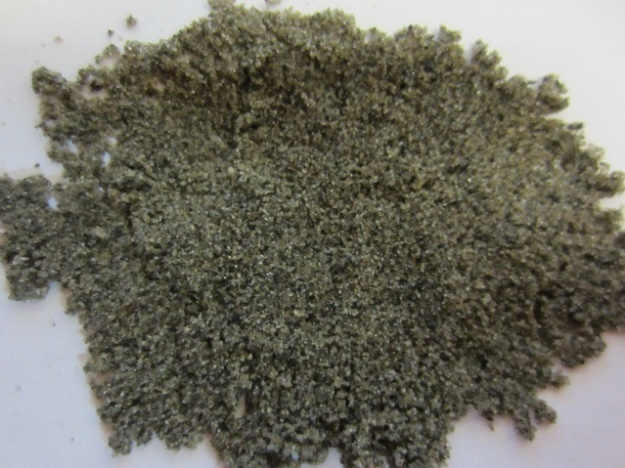
\includegraphics[width=0.5\textwidth]{figure/sand-sample.jpg}
	\caption{井筒出砂样本}
	\label{fig:sand_sample}
\end{figure}

\begin{table}[H]
	\centering
	\caption{砂砾粒度分级统计}
	\begin{tabular}{lll}
		\toprule
		分类 & 粒级区间/\(\mu\)m & 含量/\% \\
		\midrule
		砾石 & \(\leq 2000\) & 0.00 \\
		巨砂 & 2000.00--1000.00 & 0.00 \\
		粗砂 & 1000.00--500.00 & 1.03 \\
		中砂 & 500.00--250.00 & 35.29 \\
		细砂 & 250.00--125.00 & 47.15 \\
		极细砂 & 125.00--62.50 & 13.99 \\
		粗粉砂 & 62.50--31.25 & 1.92 \\
		细粉砂 & 31.25--3.90 & 0.61 \\
		粘土 & \(\leq 3.90\) & 0.00 \\
		\bottomrule
	\end{tabular}
\end{table}

\begin{table}[H]
	\centering
	\caption{仿真颗粒粒径及数量分布}
	\begin{tabular}{llll}
		\toprule
		类型 & 砂砾颗粒数量/个 & 粒径分布比例/\% & 粒径大小/\(\mu\)m \\
		\midrule
		粗砂 & 1000 & 1.0 & 750 \\
		中砂 & 35000 & 35.0 & 375 \\
		细砂 & 47000 & 47.0 & 187.5 \\
		极细砂 & 14000 & 14.0 & 93.75 \\
		粗粉砂 & 2000 & 3.0 & 46.875 \\
		\bottomrule
	\end{tabular}
\end{table}

本项目涉及到的四类工具中，“四合一”工具的外部功能单元多，结构最为复杂，在工具的几何变径处会产生边界层分离和回流现象，是砂砾沉积的“危险位置”。于是，本文选择“四合一”工具的扶正器和强磁位置作为对象，研究砂砾在此处的沉积行为。建立强磁部位与 \(7'\) 井筒环空流体仿真模型，仿真模型数据见表 1.4。研究不同环空流速下（\(\nu_{\mathrm{c}}=0.37\) m/s、\(0.59\) m/s）砂砾的运移及沉降规律，探究砂砾是否会出现沉积或者堵塞现象。计算结果如图 1.8 所示。

\begin{table}[H]
	\centering
	\caption{“四合一”工具砂砾沉积仿真模型数据}
	\begin{tabular}{llll}
		\toprule
		名称 & 符号 & 数值 & 单位 \\
		\midrule
		水平井筒长度 & \(L\) & 1.5 & m \\
		井筒直径 & \(D_{\mathrm{H}}\) & 177.8 & mm \\
		钻杆直径 & \(D_{\mathrm{P}}\) & 88.9 & mm \\
		颗粒密度 & \(\rho_{\mathrm{P}}\) & 2650.0 & kg/m\(^{3}\) \\
		压井液密度 & \(\rho_{\mathrm{l}}\) & 1000.0 & kg/m\(^{3}\) \\
		井斜角 & \(\theta\) & 90.0 & \(^{\circ}\) \\
		压井液入口流速 & \(\nu_{\mathrm{c}}\) & 0.37、0.59 & m/s \\
		压井液粘度 & \(\mu\) & 1.0 & mPa·s \\
		\bottomrule
	\end{tabular}
\end{table}

\begin{figure}[htbp]
	\centering
	
\includegraphics[width=\textwidth]{figure/tool-and-wellbore-simulation-model.png}
	\caption{工具及井筒仿真模型}
	\label{fig:tool_wellbore_model}
\end{figure}

图 1.9 描述的是压井液流速 \(0.37\) m/s 下井筒与工具环空内砂砾颗粒分布情况。从图可以看出，部分砂砾颗粒由于重力作用会在工具前端产生堆积，同时砂砾颗粒会随着工具的导流结构进行运移，在强磁部件的凹槽内也会有少量的砂砾堆积现象。

\begin{figure}[htbp]
	\centering
	
\includegraphics[width=\textwidth]{figure/sand-distribution-tool-vin-dot37.png}
	\caption{压井液流速 0.37 m/s 下井筒与工具环空内砂砾颗粒分布}
	\label{fig:sand_distribution_tool_vin_dot37}
\end{figure}

图 1.10 描述的是相同时间步环空流速 \(0.37\) m/s、\(0.59\) m/s 下砂砾颗粒分布。从图中可以看出，环空流速增大时，靠近压力出口的砂砾颗粒越多，砂砾颗粒的运移效率明显加快。在相同时间步下，环空流速越大，颗粒运移速度越快。由于环空流速增大，流体的拖曳力增大，砂砾颗粒在轴向的速度增大，砂砾颗粒由于重力作用产生的沉积位置与流体入口的距离也变远。

\begin{figure}[htbp]
	\centering
	\subfloat[环空流速 0.37 m/s]{%
		
\includegraphics[width=0.98\textwidth]{figure/sand-distribution-annular-vin-dot37.png}
		\label{fig:sand_distribution_annular_vin_dot37}
	}
	\vspace{0pt}
	\subfloat[环空流速 0.59 m/s]{%
		
\includegraphics[width=0.98\textwidth]{figure/sand-distribution-annular-vin-dot59.png}
		\label{fig:sand_distribution_annular_vin_dot59}
	}
	\caption{相同时间步不同环空流速下砂砾颗粒分布}
	\label{fig:sand_distribution_annular_vin}
\end{figure}

通过仿真发现，在冲砂作业时，如果环空流体中砂砾体积分数越大，越容易在工具与井筒下壁之间的环空中产生沉积，环空流速增大，砂砾运移效率加快，建议在作业时增大压井液流速即增大冲砂液排量以减小砂砾堆积的风险，降低砂堵概率。同时，工具的导流结构也对砂砾运移起到关键作用，砂砾颗粒会随着工具的导流结构进行运移，降低了砂堵的风险，为工具安全作业提供保障。

上述研究仅仅从宏观上观测砂砾在井筒环空中的运移情况，无法提取井筒环空中不同具体位置的砂砾体积分数、砂砾速度及砂砾床厚度等数据。为此，本研究考虑井筒环空不同位置的砂砾量，基于欧拉液固两相流模型和 \(SST k-\omega\) 模型，建立了三维井眼环空颗粒运移模型，在分析砂砾体积分数和砂砾速度的基础上，通过 Fluent 分析整个环空中砂砾质量，提出了环空内含有颗粒质量的变化方法，分析了幂律流体中环空流速、井斜角度、压井液粘度等对环空内沉降的砂床高度的影响。所得结论对水平井和大位移井环空内井筒清洁和高效作业具有指导意义。

\subsection{数值模型建立}

根据实际工况，在钻井过程中，钻井液携带砂砾颗粒进入环空，因此内部环境为复杂的液--固两相流湍流流场，故选用 Eulerian 两相流模型对环空砂砾运移进行数值模拟，将环空流场视为稳定的不可压缩湍流流场。

\subsubsection{幂律流体}

钻井液属于非牛顿流体，其本构方程符合幂律流体，流变参数
\begin{equation}
	\tau=K\dot{\gamma}^{n}
\end{equation}
其中，\(K\) 为钻具内钻井液稠度系数，\(n\) 为钻井液流变指数。依据相关文献，\(K=2.38\)，\(n=0.80\)。

\subsection{几何模型及边界条件}

\subsubsection{几何模型}

根据现场实际油井组合参数建立环空三维模型，如图 1.11 所示。实际水平井段很长，为了研究方便，取水平井模型长 \(1.5\) m，取曲率半径 \(1\) m、曲率为 \(90^{\circ}\) 的圆弧弯管模型模拟不同井斜角度，考虑井壁和钻杆表面光滑，计算流域由钻杆和井壁表面组成。采用多面体单元对所建模型进行网格划分。

\begin{figure}[htbp]
	\centering
	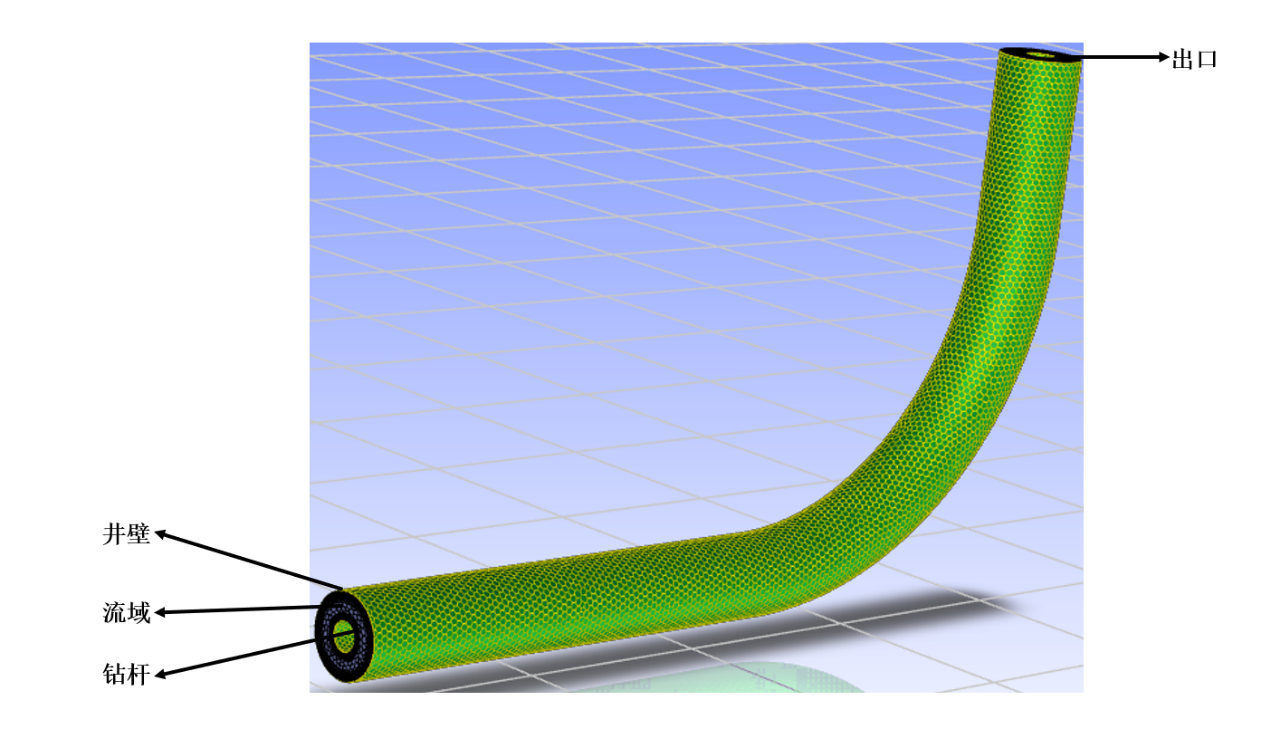
\includegraphics[width=0.8\textwidth]{figure/annular-3d-model.png}
	\caption{环空三维模型}
	\label{fig:annular_3d_model}
\end{figure}

\subsubsection{边界条件}

考虑模拟运算中的收敛性和稳定性，湍流流场的计算采用二阶迎风格式和 SIMPLE 算法。根据实际工况对模型入口边界条件定义，具体为：压井液速度入口和砂砾颗粒入口；出口边界条件为 outlet；将井壁与钻杆表面设为 stationary wall。具体模拟参数如下：井眼直径 244.475 mm，钻杆直径 88.9 mm，砂砾密度 \(2650\) kg/m\(^{3}\)，压井液密度 1000、1300、1400 kg/m\(^{3}\)，砂砾直径 250 \(\mu\)m，钻井液入口排量 25、40、100 m\(^{3}\)/h，压井液粘度为 1、2.3、5 cp。

\subsection{数值模拟及结果分析}

\subsubsection{环空砂砾沉降分析}

通过对井筒环空内砂砾质量进行仿真，得到钻杆静止时环空内砂砾沉降质量变化曲线，如图 1.12 所示。由图可知，环空内砂砾质量曲线先呈线性增长，在 30 s 后不再继续增长，而是随时间在稳定值上下波动。这说明井筒内进入的砂砾量与出口排出的砂砾量接近，可判断环空内沉积的砂砾量达到稳定值，平均岩屑质量为 \(63.294\) kg。

\begin{figure}[htbp]
	\centering
	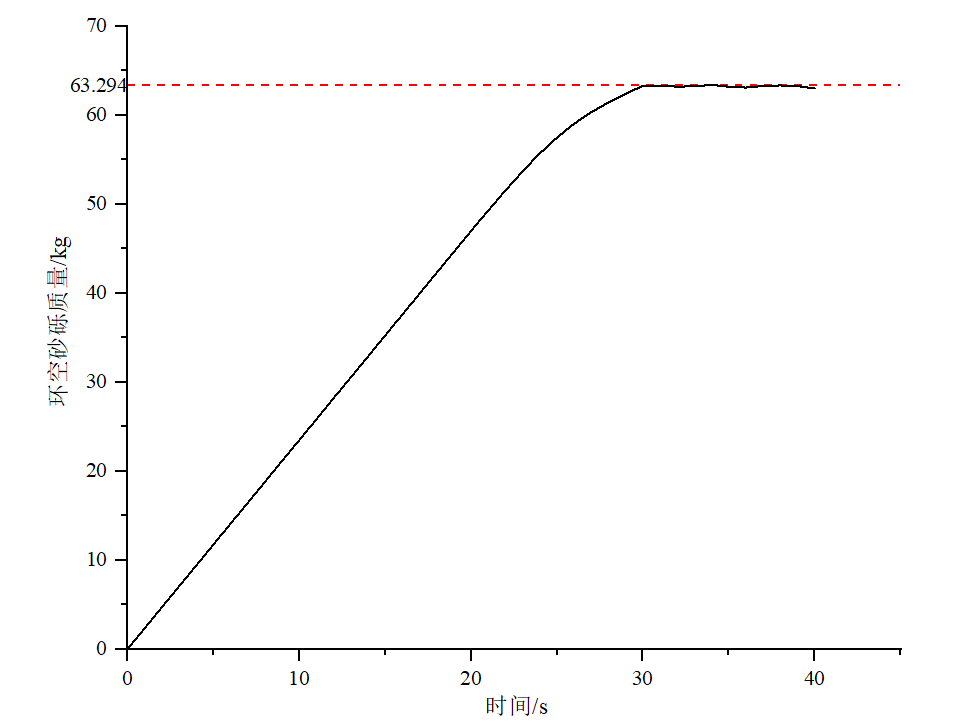
\includegraphics[width=0.7\textwidth]{figure/sand-mass-in-annular-VS-time.png}
	\caption{环空内砂砾质量变化曲线}
	\label{fig:sand_mass_in_annular_VS_time}
\end{figure}

图 1.13 和图 1.14 分别为不同位置截面砂砾轴向速度云图和砂砾体积分数云图。其中水平段每个截面间距 \(500\) mm，井斜段井斜角度间隔 \(15^{\circ}\)，且距离入口 500、1000、1500 mm 处，井斜段 \(15^{\circ}\)、\(30^{\circ}\)、\(75^{\circ}\) 处截面进行放大。环空中砂砾量达到稳定后，由于整个环空中的砂砾不是均匀分布，所以不同位置砂砾速度和体积分数有一定差异。由图可知：环空上部为流体高速区，流速大；下部为低速区，流速趋近于 0。由于重力作用，砂砾趋向环空下部，大部分砂砾沉降在环空下部低速区，造成砂砾难以运移，最终形成砂砾床。

\begin{figure}[htbp]
	\centering
	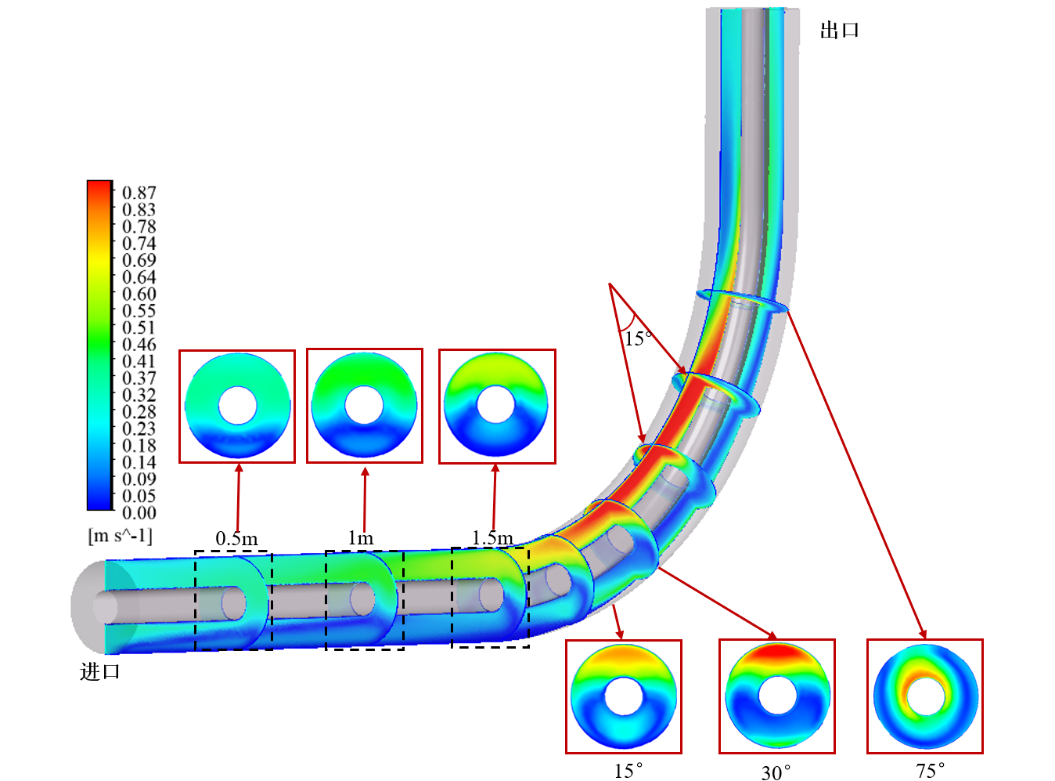
\includegraphics[width=0.8\textwidth]{figure/sand-velocity-cloud-sections.png}
	\caption{不同截面砂砾速度云图}
	\label{fig:sand_velocity_cloud_sections}
\end{figure}

\begin{figure}[htbp]
	\centering
	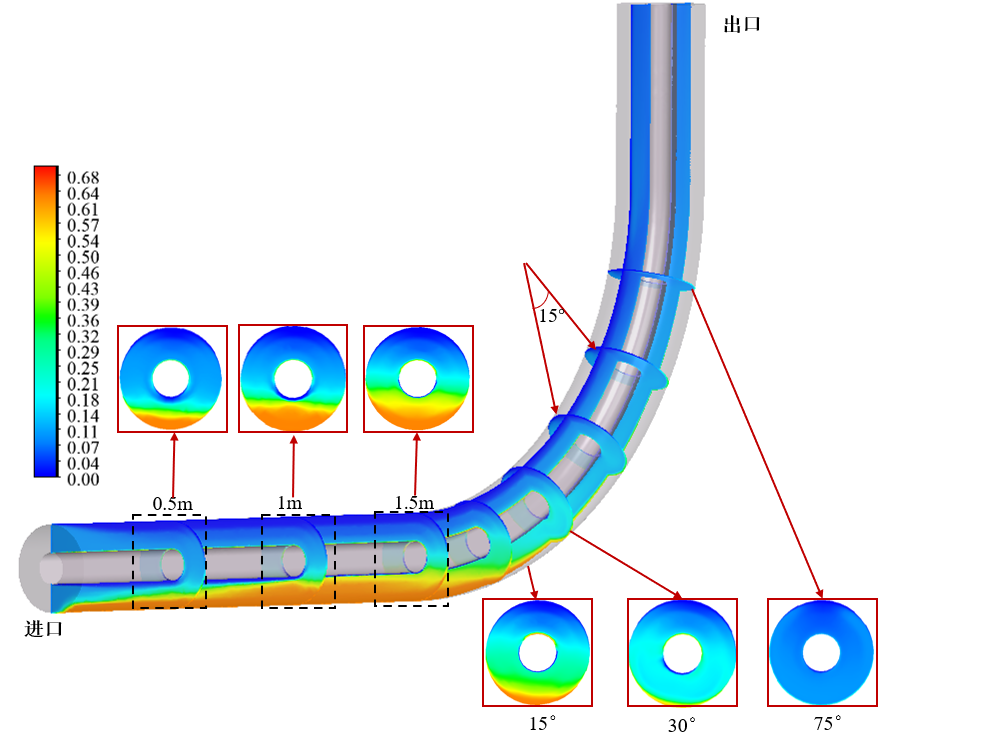
\includegraphics[width=0.8\textwidth]{figure/sand-volume-fraction-cloud-sections.png}
	\caption{不同截面砂砾体积分数云图}
	\label{fig:sand_volume_fraction_cloud_sections}
\end{figure}

\subsubsection{压井液流速对环空砂砾沉积的影响}

图 1.15 为粘度 \(2.3\) cp，排量 25、40、100 m\(^{3}\)/h（0.17、0.27、0.69 m/s）时，不同流速下环空内砂砾质量随时间的变化曲线。由图可以看出，随着时间的延长，环空内沉降的砂砾质量趋于稳定，并且随着流速升高，环空内沉降的砂砾质量减小，且到达稳定的时间加快。

\begin{figure}[htbp]
	\centering
	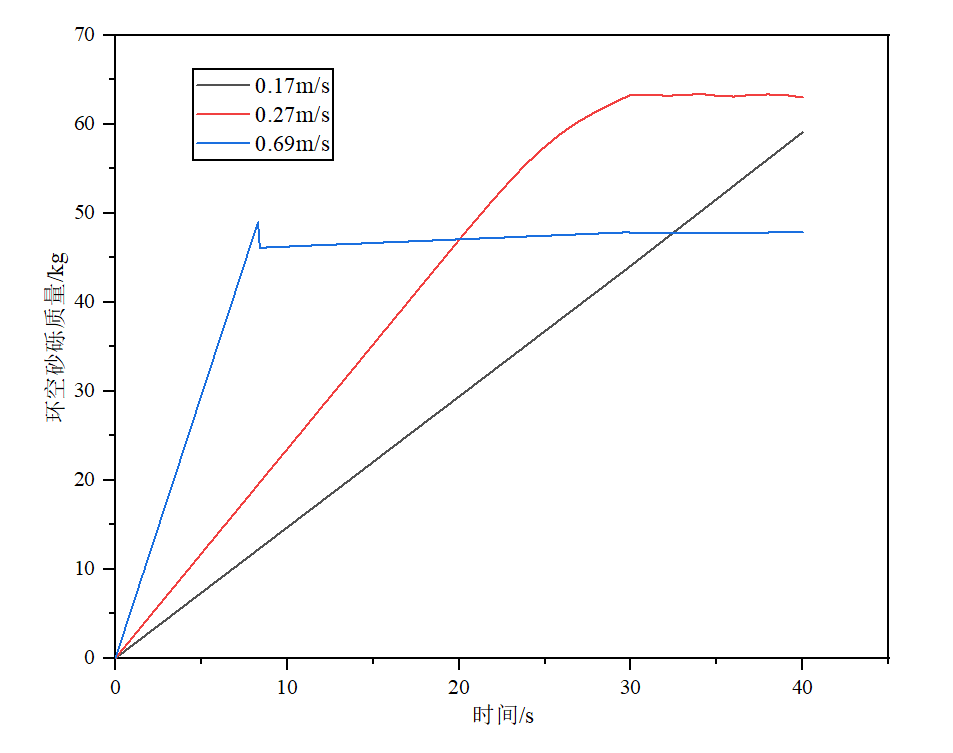
\includegraphics[width=0.7\textwidth]{figure/sand-mass-in-annular-VS-time-flowrate.png}
	\caption{不同流速下环空内砂砾质量随时间的变化曲线}
	\label{fig:sand_mass_in_annular_VS_time_flowrate}
\end{figure}

假设环空内体积分数最大且沉积高度最高的位置为最容易发生砂堵位置，定为 block 点（简称 b 点）。图 1.16 为流速为 \(0.17\) m/s 时环空内砂砾的体积分数云图，则流速为 \(0.17\) m/s 时，b 点出现在水平段距离入口 \(1280\) mm 处，高度为 \(68\) mm。砂砾床主要沉积在水平段，随着井斜角度增加，砂砾体积分数逐渐减小，井斜 \(75^{\circ}\) 时，砂砾体积分数接近于 0。

\begin{figure}[htbp]
	\centering
	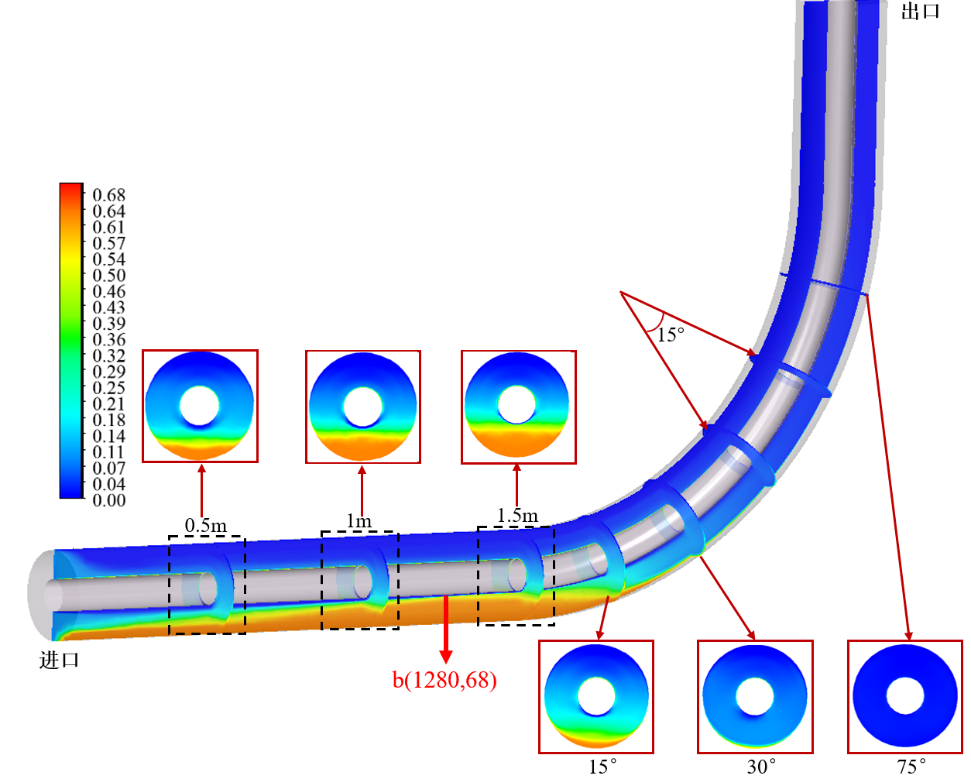
\includegraphics[width=0.7\textwidth]{figure/sand-volume-fraction-vin-dot17.png}
	\caption{流速为 0.17 m/s 时环空内砂砾的体积分数云图}
	\label{fig:sand_volume_fraction_vin_dot17}
\end{figure}

图 1.17 为流速为 \(0.27\) m/s 时环空内砂砾的体积分数云图，流速为 \(0.27\) m/s 时，b 点出现在水平段距离入口 \(1150\) mm 处，高度为 \(64\) mm。砂砾床主要沉积在水平段，相对于 \(0.17\) m/s 流速工况，砂砾在井斜段体积分数有所增加，砂砾向出口运移的效率增大。

\begin{figure}[htbp]
	\centering
	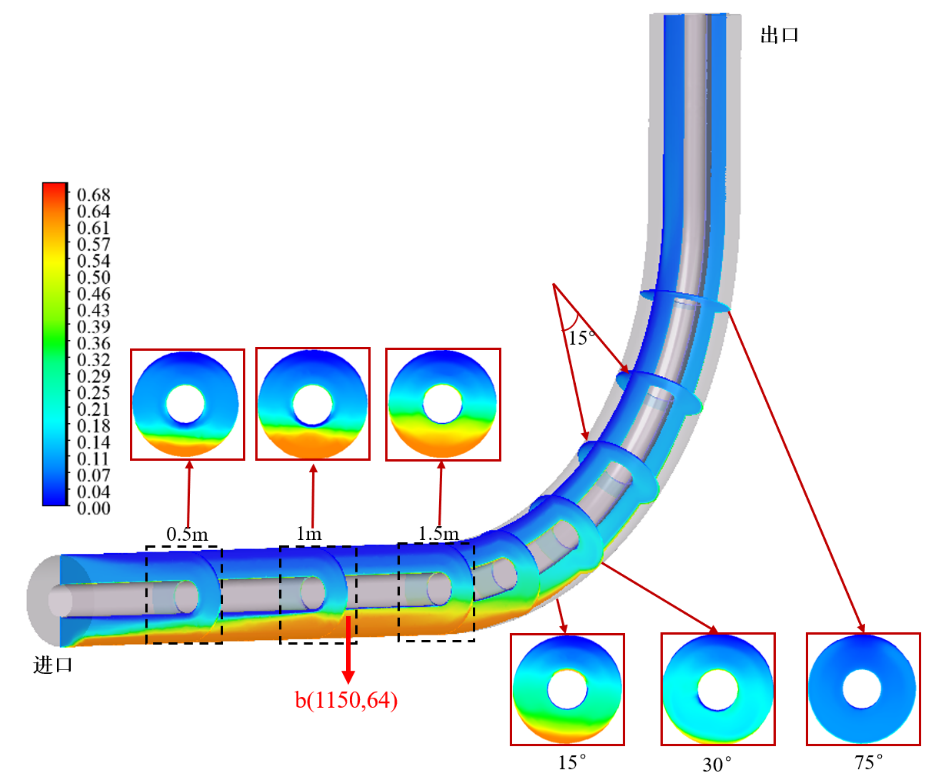
\includegraphics[width=0.7\textwidth]{figure/sand-volume-fraction-vin-dot27.png}
	\caption{流速为 0.27 m/s 时环空内砂砾的体积分数云图}
	\label{fig:sand_volume_fraction_vin_dot27}
\end{figure}

图 1.18 为流速为 \(0.69\) m/s 时环空内砂砾的体积分数云图，流速为 \(0.69\) m/s 时，b 点出现在水平段距离入口 \(1530\) mm 处，高度为 \(32\) mm。砂砾床沉积在水平段及小倾角井斜段，砂砾床高度明显降低，砂堵风险明显下降，且井斜段砂砾体积分数明显增大，砂砾运移效率增大。

\begin{figure}[htbp]
	\centering
	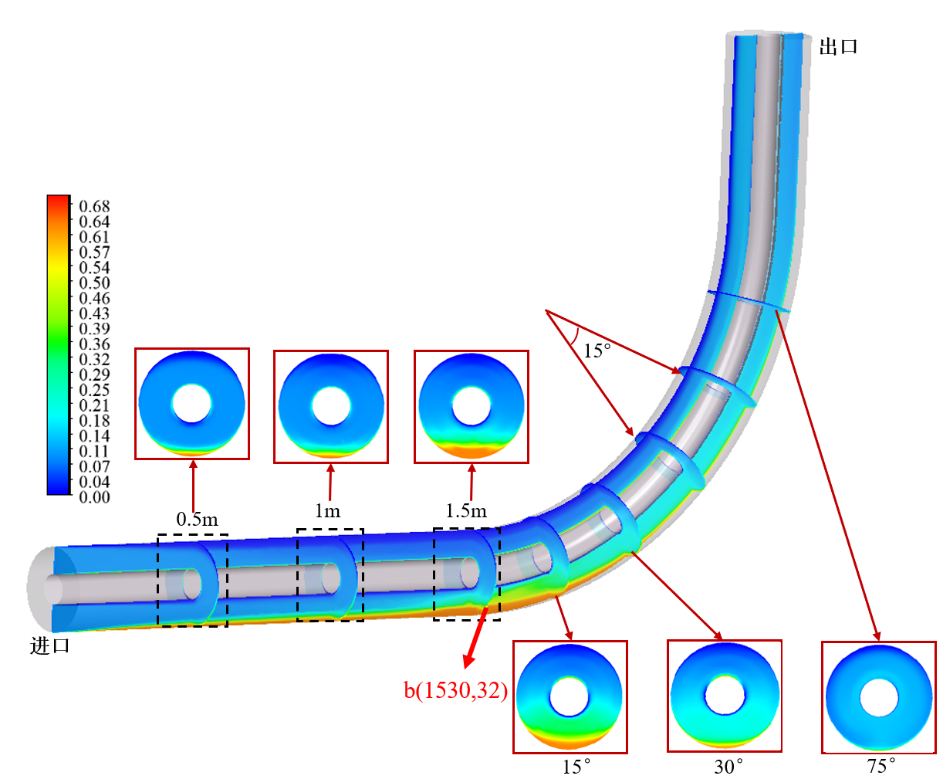
\includegraphics[width=0.7\textwidth]{figure/sand-volume-fraction-vin-dot69.png}
	\caption{流速为 0.69 m/s 时环空内砂砾的体积分数云图}
	\label{fig:sand_volume_fraction_vin_dot69}
\end{figure}

图 1.19 为 b 点高度随压井液流速变化曲线，由图中可以看到随着压井液流速增大，b 点高度逐渐减小。

\begin{figure}[htbp]
	\centering
	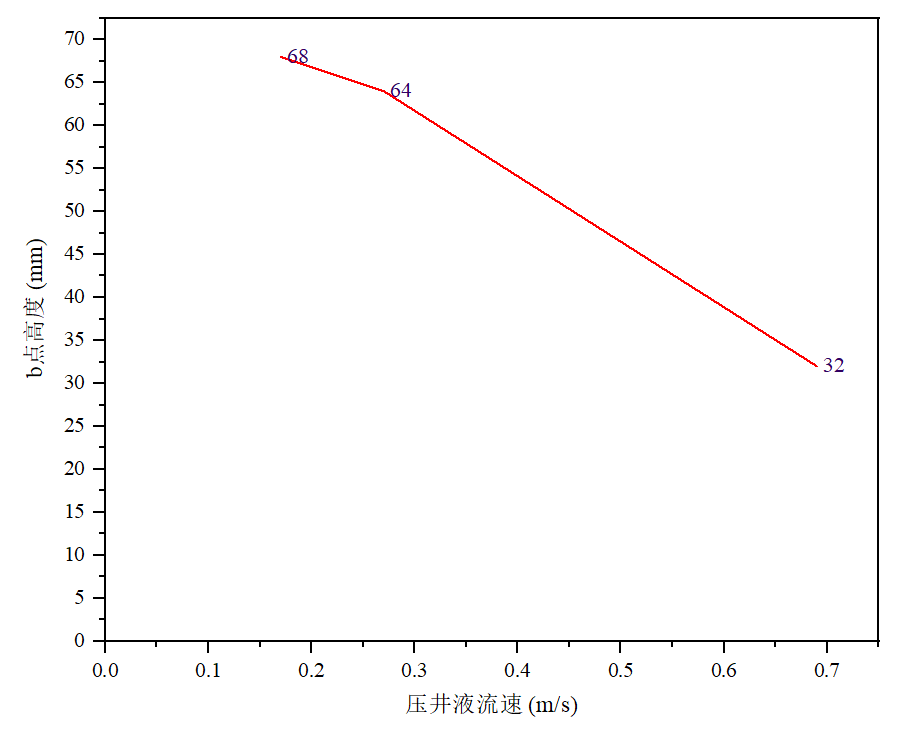
\includegraphics[width=0.7\textwidth]{figure/b-point-height-VS-flowrate.png}
	\caption{b 点高度随压井液流速变化曲线}
	\label{fig:b_point_height_VS_flowrate}
\end{figure}

图 1.20 为 b 点不同压井液流速下砂砾体积分数和轴向速度云图，随着压井液流速增大，b 点砂砾体积分数减小，且砂砾流速增大，这说明环空排量的增大，增强了流体的携砂能力，促进了砂砾颗粒在环空中的流动性，增加了砂砾颗粒能量，为砂砾运移提供了更大的拖曳力，从而有效地提高了井筒内砂砾颗粒的运移效率。因此在实际作业中，要想减小砂堵风险，宜尽量采用更大的冲砂排量。

\begin{figure}[htbp]
	\centering
	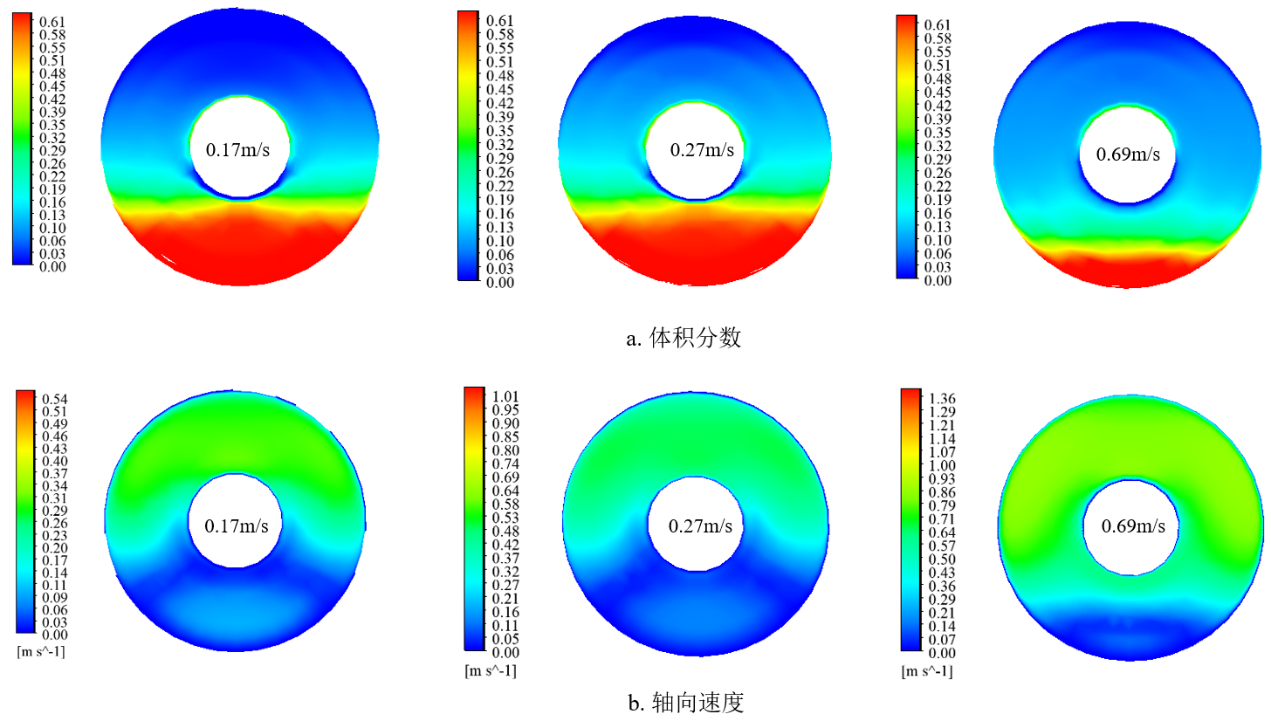
\includegraphics[width=0.8\textwidth]{figure/sand-volume-fraction-velocity-at-b-point-flowrate.png}
	\caption{b 点不同压井液流速下砂砾体积分数和轴向速度云图}
	\label{fig:sand_volume_fraction_velocity_at_b_point_flowrate}
\end{figure}

\subsubsection{压井液粘度对环空砂砾沉积的影响}

图 1.21 为流速 \(0.27\) m/s 时，粘度分别取 1.0、2.3、5.0 cp 时，不同粘度下环空内砂砾质量随时间的变化曲线。由图可以看出，随着时间的延长，环空内沉降的砂砾质量趋于稳定，并且随着粘度增大，环空内沉降的砂砾质量减小，且到达稳定的时间加快。

\begin{figure}[htbp]
	\centering
	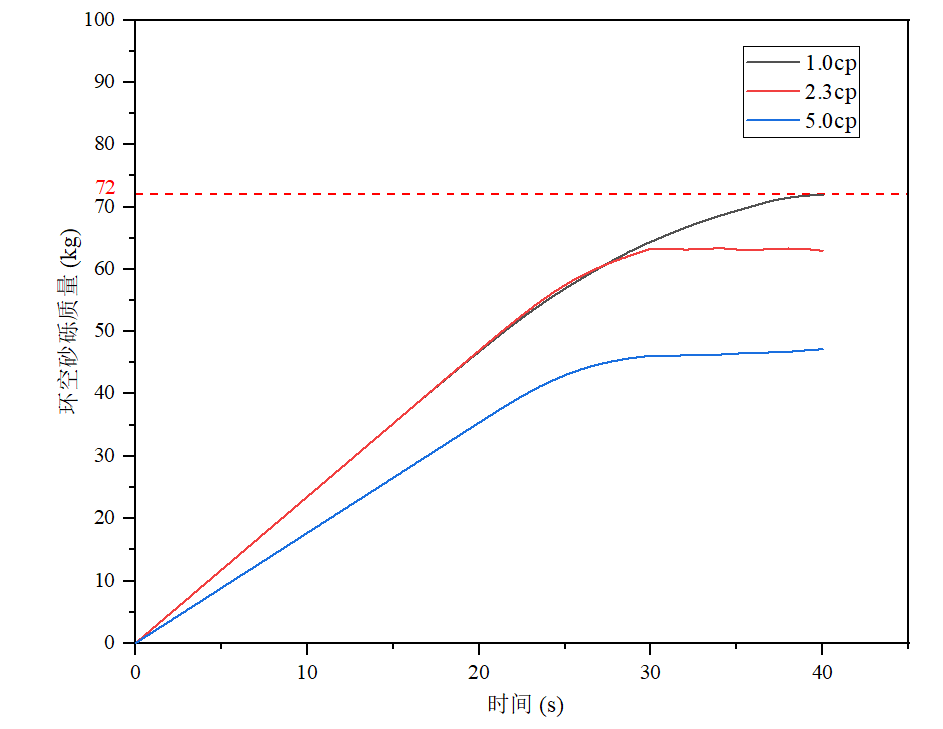
\includegraphics[width=0.7\textwidth]{figure/sand-mass-in-annular-VS-time-viscosity.png}
	\caption{不同粘度下环空内砂砾质量随时间的变化曲线}
	\label{fig:sand_mass_in_annular_VS_time_viscosity}
\end{figure}

图 1.22 为粘度为 \(1.0\) cp 时环空内砂砾的体积分数云图，则粘度为 \(1.0\) cp 时，b 点出现在水平段距离入口 \(800\)--\(1400\) mm 处，高度为 \(77.5\) mm。砂砾床主要沉积在水平段，随着井斜角度增加，砂砾体积分数逐渐减小，井斜 \(75^{\circ}\) 时，砂砾体积分数接近于 0。

\begin{figure}[htbp]
	\centering
	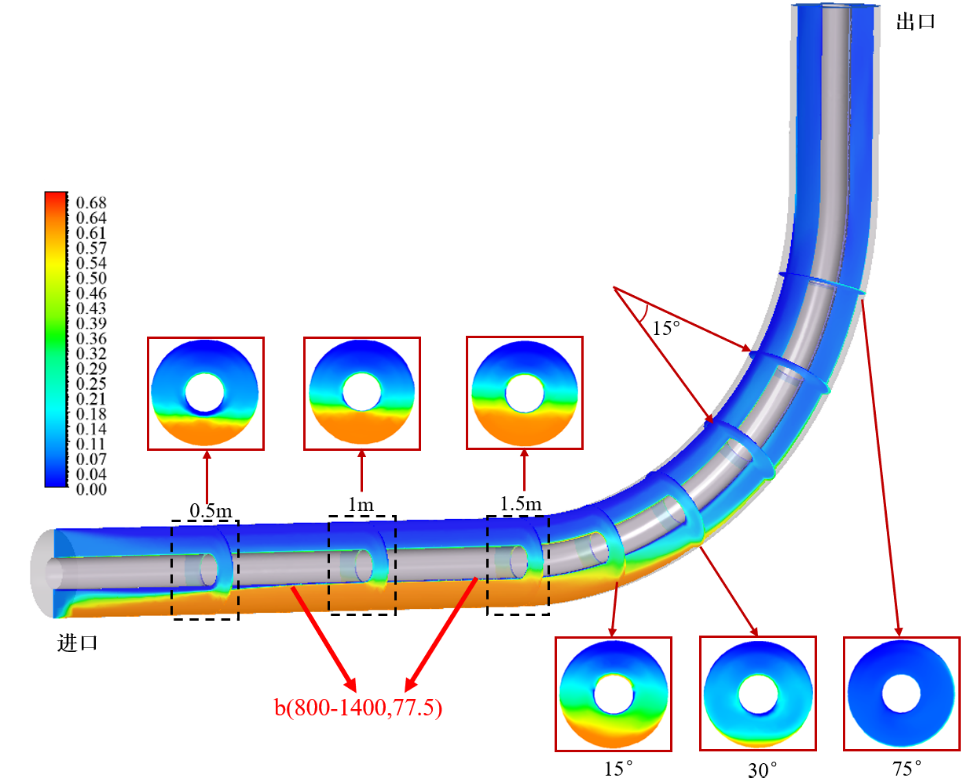
\includegraphics[width=0.7\textwidth]{figure/sand-volume-fraction-mu-1cp.png}
	\caption{粘度为 1.0 cp 时环空内砂砾的体积分数云图}
	\label{fig:sand_volume_fraction_mu_1cp}
\end{figure}

图 1.23 为粘度为 \(5.0\) cp 时环空内砂砾的体积分数云图，则粘度为 \(5.0\) cp 时，b 点出现在水平段距离入口 \(1000\) mm 处，高度为 \(25\) mm。砂砾床沉积在水平段及小倾角井斜段，砂砾床高度明显降低，砂堵风险明显下降，且井斜段砂砾体积分数明显增大，砂砾运移效率增大。

\begin{figure}[htbp]
	\centering
	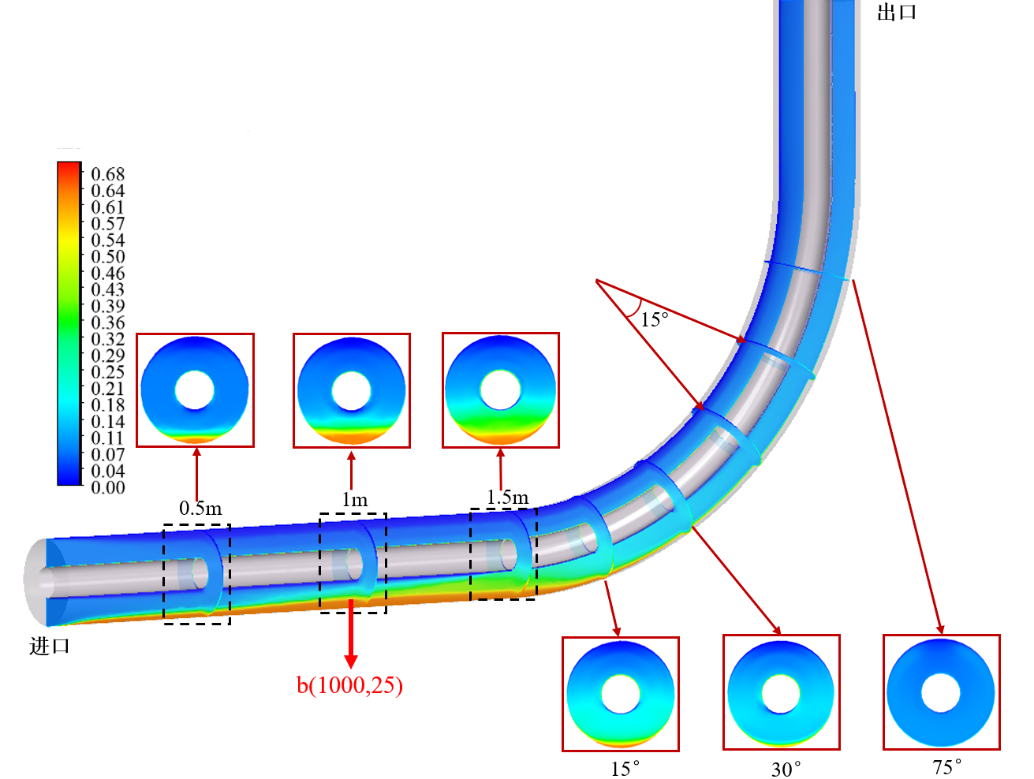
\includegraphics[width=0.7\textwidth]{figure/sand-volume-fraction-mu-5cp.png}
	\caption{粘度为 5.0 cp 时环空内砂砾的体积分数云图}
	\label{fig:sand_volume_fraction_mu_5cp}
\end{figure}

图 1.24 为 b 点高度随压井液粘度变化曲线，由图中可以看到随着压井液粘度增大，b 点高度逐渐减小。

\begin{figure}[htbp]
	\centering
	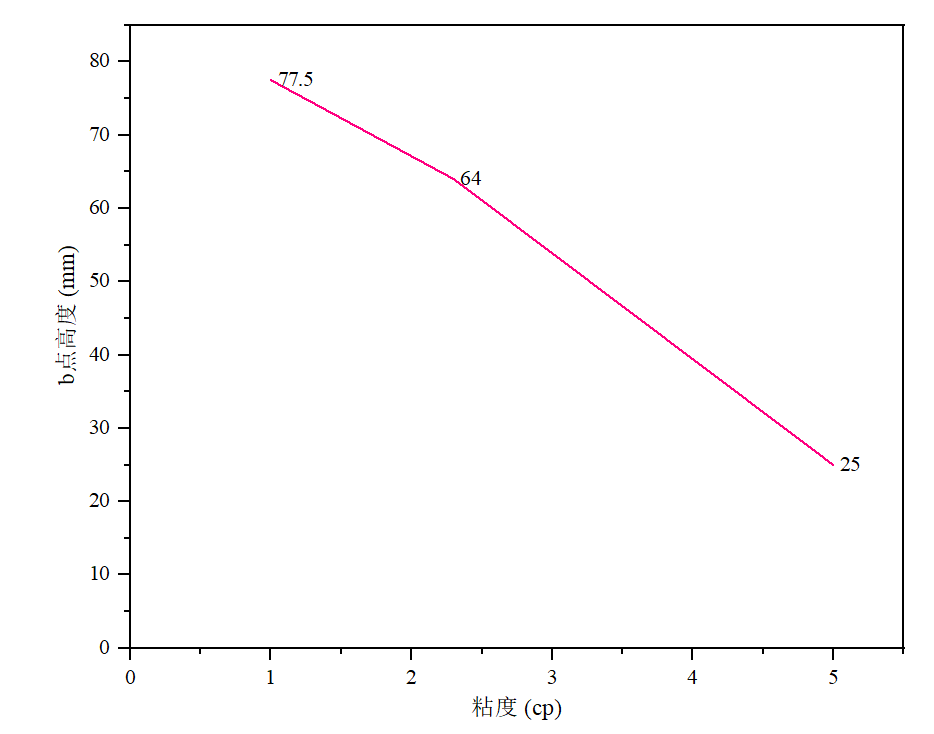
\includegraphics[width=0.7\textwidth]{figure/b-point-height-VS-viscosity.png}
	\caption{b 点高度随压井液粘度变化曲线}
	\label{fig:b_point_height_VS_viscosity}
\end{figure}

图 1.25 为 b 点不同压井液粘度下砂砾体积分数和轴向速度云图，随着压井液粘度增大，b 点砂砾体积分数减小，但砂砾流速有减小的趋势，这说明压井液粘度的增大，增大了流体的携砂能力，但是会减小环空中流体的流动性，这说明增大压井液粘度可以抑制砂堵在井底的形成，但是也会增加砂砾上返的时间。因此在实际作业中，要想减小砂堵风险，宜采用粘度更大的压井液。

\begin{figure}[htbp]
	\centering
	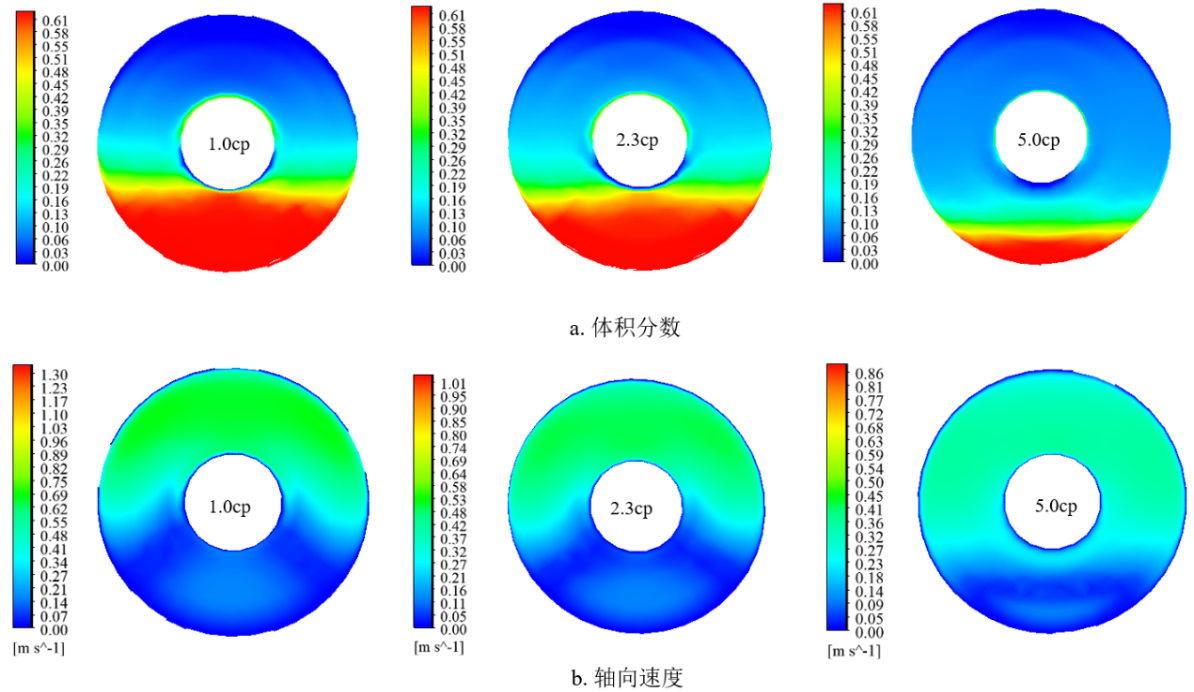
\includegraphics[width=0.8\textwidth]{figure/sand-volume-fraction-velocity-at-b-point-viscosity.png}
	\caption{b 点不同压井液粘度下砂砾体积分数和轴向速度云图}
	\label{fig:sand_volume_fraction_velocity_at_b_point_viscosity}
\end{figure}

\section{井筒内铁屑运移及分布规律}
%20260704想法：仿真->实验->外推。这个研究属于“基础性研究”（与4.适用条件中“拓深技术理论及基础性研究”对应），界定了研究的性质——是基础理论研究，不是工程应用。目的是“揭示影响工具应用效果的主控因素”，对应5.1.2 ①的要求是“研究不同流速、粘度、井斜下的运移规律”，通过实验验证哪些参数是影响运移的“主控因素”（Re（实验已经证明）、井斜角的影响在全井筒模型实验中展示）。

在井下封隔器套铣作业过程中，将产生包含多种形态碎屑的混合物（见图\ref{fig:iron_shavings_sample}），其中，金属碎屑（尤其是铁屑）不仅可能导致筛管堵塞风险，还可能导致工具活动部件卡滞。经磨铣封隔器作业上返的碎屑样本分析表明，金属碎屑主要包含环状颗粒、块状颗粒及丝状颗粒三种形态。其中，丝状铁屑因其特有的几何特征，易通过旋转与缠绕作用形成网状结构，从而显著提升孔隙滞留概率。该类颗粒的高长径比特性不仅加剧了运移过程的复杂性，其各向异性运动模式及增大的比表面积更强化了流体拖曳力与壁面吸附效应，为油井金属碎屑对流动通道的动态阻塞机制提供了更真实的物理表征。基于上述特性分析，本研究选取丝状铁屑作为典型颗粒开展建模研究，具体模型及参数见图\ref{fig:iron_particle_comparison}和表\ref{tab:simulation_params}。

\begin{figure}[htbp]
    \centering
    
\includegraphics[width=0.5\textwidth]{figure/iron-shavings-sample.jpg}
    \caption{井下封隔器套铣作业中产生的金属碎屑样本}
    \label{fig:iron_shavings_sample}
\end{figure}

\begin{figure}[htbp]
    \centering
    % 子图 (a)
    \subfloat[实际铁屑颗粒]{%
        \begin{minipage}[t]{0.48\linewidth}
            \centering
            
\includegraphics[width=\linewidth]{figure/iron-wire-actual.jpg}
            \label{fig:actual}
        \end{minipage}%
    }
    \hfill
    % 子图 (b)
    \subfloat[铁屑颗粒模型]{%
        \begin{minipage}[t]{0.45\linewidth}
            \centering
            
\includegraphics[width=\linewidth]{figure/iron-wire-model.jpg}
            \label{fig:model}
        \end{minipage}%
    }
    % 总标题
    \caption{铁屑颗粒及仿真模型}
    \label{fig:iron_particle_comparison}
\end{figure}

\begin{table}[htbp]
    \centering
    \caption{铁屑颗粒运移仿真参数}
    \label{tab:simulation_params}
    % 设置列格式：
    % c: 居中
    % p{width}: 固定宽度并自动换行（适合较长的中文名称）
    \begin{tabularx}{.9\textwidth}{cccXc} 
        \toprule % 绘制顶部粗线
        % 表头部分
        序号 & 名称 & 符号 & 数值 & 单位 \\ 
        \midrule % 绘制中间细线
        
        % 数据行
        1 & 水平井筒长度 & $L$ & 1.5 & m \\
        2 & 井筒直径 & $D_H$ & 244.475 & mm \\
        3 & 钻杆直径 & $D_P$ & 88.9 & mm \\
        4 & 颗粒密度 & $\rho_p$ & 7800.0 & kg/m$^3$ \\
        5 & 压井液密度 & $\rho_l$ & 1000.0、1300.0 & kg/m$^3$ \\
        6 & 井斜角 & $\theta$ & 0.0、45.0、90.0 & $^\circ$ \\
        7 & 压井液入口流速 & $v_{in}$ & 0.17、0.27 & m/s \\
        8 & 压井液粘度 & $\mu$ & 1.0、1.7 & mPa$\cdot$s \\
        9 & 沉积域距离井壁高度 & $H$ & 40.0 & mm \\
        10 & 颗粒与井壁静摩擦系数 & $\mu_s$ & 0.15 & - \\
        11 & 颗粒与井壁滑动摩擦系数 & $\mu_k$ & 0.1 & - \\
        
        \bottomrule % 绘制底部粗线
    \end{tabularx}
\end{table}

\subsection{压井液粘度对铁屑运移规律的影响}
本节选取清水和氯化钠溶液（相对密度为1.3）两种压井液进行对比。二者均可视为牛顿流体，但粘度不同，对铁屑颗粒的携带效果可能存在差异。在$\theta=90^\circ$、$v_{\mathrm{in}}=0.27\mathrm{m/s}$的条件下，通过仿真对比二者的携屑效果。图\ref{fig:iron_wire_distribution_viscosity}描述的是不同压井液粘度下井筒内铁屑的分布情况（以颗粒速度着色）。从图中可以看出，压井液粘度对铁屑颗粒运移效率的影响不大：随着压井液粘度增大，移动铁屑床的速度略微增大，颗粒运移效率略有提高，出口处的铁屑颗粒有所增多。
%通过对不同压井液的性能特点进行分析，可以为选择最适合的压井液粘度提供参考，从而优化洗井操作并提高效率。

\begin{figure}[htbp]
    \centering
    % --- 子图 (a) ---
    % 使用 minipage 控制宽度，这里设为 0.9\textwidth 让图片大一点
    % [t] 表示顶部对齐，防止因为图片高度不同导致错位
    \subfloat[$\mu = 1.0\mathrm{mPa}\cdot\mathrm{s}$]{
        \begin{minipage}[t]{0.8\linewidth}
            \centering
            % 替换为你的第一张图片文件名
            
\includegraphics[width=\linewidth]{figure/iron-wire-distribution-1cp-velocity-colored.png} 
            \label{fig:viscosity_1.0}
        \end{minipage}
    }
    \vspace{0pt} % 上下两张图之间的垂直间距，可根据需要调整
    % --- 子图 (b) ---
    \subfloat[$\mu = 1.7\mathrm{mPa}\cdot\mathrm{s}$]{
        \begin{minipage}[t]{0.8\linewidth}
            \centering
            % 替换为你的第二张图片文件名
            
\includegraphics[width=\linewidth]{figure/iron-wire-distribution-1dot7-cp-velocity-colored.png} 
            \label{fig:viscosity_1.7}
        \end{minipage}
    }
    % --- 总标题 ---
    \caption{压井液粘度对铁屑颗粒速度分布的影响（$\theta=90^\circ$,\ $v_{\mathrm{in}}=0.27\mathrm{m/s}$）}
    \label{fig:iron_wire_distribution_viscosity}
\end{figure}

图\ref{fig:iron_wire_mean_velocity_evolution_viscosity}为两种压井液粘度下井筒稳态后铁屑颗粒沉积域铁屑颗粒运移速度图。从图中可以看出，$\mu$从$1.0\mathrm{mPa\cdot s}$增加到$1.7\mathrm{mPa\cdot s}$时，粘度增加到$1.7$倍，但铁屑的平均运移速度只增加到$1.04$倍，证明压井液的粘度对铁屑运移的影响十分有限。
\begin{figure}[htbp]
    \centering
    
\includegraphics[width=0.7\textwidth]{figure/iron-wire-mean-velocity-evolution-viscosity.jpg}
    \caption{压井液粘度对铁屑颗粒运移速度时间演变的影响（$\theta=90^\circ$,\ $v_{\mathrm{in}}=0.27\mathrm{m/s}$）}
    \label{fig:iron_wire_mean_velocity_evolution_viscosity}
\end{figure}

\subsection{压井液流速对铁屑运移规律的影响}

本节探究压井液流速对井筒环形空间内铁屑颗粒运移的影响。选取了水平段为研究对象，给定$\mu=1.7\mathrm{mPa\cdot s}$。

图\ref{fig:iron_wire_distribution_velocity}描述的是两种流速下井筒内铁屑颗粒分布情况，入口流速对铁屑颗粒运移行为的影响显著。铁屑的密度较大，在两种进口流速下，均表现出在边运移边沉积的现象，在水平管的底部位置有形成颗粒床的趋势。
随着压井液流速的增加，从颗粒工厂出发的铁屑颗粒整体上产生了更大的轴向位移，颗粒整体的瞬时速度也有增加的趋势。这是由于压井液流速增大时，铁屑颗粒受到流体沿轴向给予的拖拽力增加，铁屑颗粒沿轴向运移的速度增加。同时，增大的拖拽力也能对抗管壁摩擦效应，颗粒的运移效率增加。
\begin{figure}[htbp]
    \centering
    % --- 子图 (a) ---
    % 使用 minipage 控制宽度，这里设为 0.9\textwidth 让图片大一点
    % [t] 表示顶部对齐，防止因为图片高度不同导致错位
    \subfloat[$v_{\mathrm{in}} = 0.17\mathrm{m/s}$]{
        \begin{minipage}[t]{0.8\linewidth}
            \centering
            % 替换为你的第一张图片文件名
            
\includegraphics[width=\linewidth]{figure/iron-wire-distribution-1dot7cp-0dot17mpers.png} 
            \label{fig:distribution_velocity_0.17}
        \end{minipage}
    }
    \vspace{0pt} % 上下两张图之间的垂直间距，可根据需要调整
    % --- 子图 (b) ---
    \subfloat[$v_{\mathrm{in}} = 0.27\mathrm{m/s}$]{
        \begin{minipage}[t]{0.8\linewidth}
            \centering
            % 替换为你的第二张图片文件名
            
\includegraphics[width=\linewidth]{figure/iron-wire-distribution-1dot7cp-0dot27mpers.png} 
            \label{fig:distribution_velocity_0.27}
        \end{minipage}
    }
    % --- 总标题 ---
    \caption{压井液流速对铁屑颗粒分布的影响（$\theta=90^\circ$,\ $\mu = 1.7\mathrm{mPa}\cdot\mathrm{s}$）}
    \label{fig:iron_wire_distribution_velocity}
\end{figure}

铁屑颗粒的运动迹线图直观地展现了颗粒的运动轨迹，本文选取了井筒内的部分铁屑颗粒，绘制了两种流速下其迹线图，如图\ref{fig:iron_wire_particle_track_velocity}所示。从图中可以看出，在颗粒工厂中产生的铁屑颗粒一经产生，将很快获得轴向移动速度，这一点可从左上至右下的迹线得到证明；且进口流速越大，迹线的斜率越小，颗粒获得的周向速度也越大。在两种情况下，颗粒落到管底后，以较大幅度弹跳的方式向前运动，而非形成密实的颗粒床以整体的形式运动。在图\ref{fig:distribution_velocity_0.27}中，铁屑颗粒在颗粒工厂右边界附近的迹线混叠密度也低于前者，说明进口流速提升时，颗粒得以弥散开来，颗粒床的形成受到了抑制。

%这两张图的总仿真时间是个很重要的变量。第一个总的仿真时间长，第二个总的仿真时间短。总仿真时间长，颗粒的运动轨迹就会更长，颗粒的运动轨迹就会更密集。总仿真时间短，颗粒的运动轨迹就会更短，颗粒的运动轨迹就会更稀疏。

\begin{figure}[htbp]
	\centering
	% --- 子图 (a) ---
	% 使用 minipage 控制宽度，这里设为 0.9\textwidth 让图片大一点
	% [t] 表示顶部对齐，防止因为图片高度不同导致错位
	\subfloat[$v_{\mathrm{in}} = 0.17\mathrm{m/s}$]{
		\begin{minipage}[t]{0.8\linewidth}
			\centering
			% 替换为你的第一张图片文件名
			
\includegraphics[width=\linewidth]{figure/iron-wire-particle-track-1dot7cp-0dot17mpers.jpg} 
			\label{fig:track_velocity_0.17}
		\end{minipage}
	}
	\vspace{0pt} % 上下两张图之间的垂直间距，可根据需要调整
	% --- 子图 (b) ---
	\subfloat[$v_{\mathrm{in}} = 0.27\mathrm{m/s}$]{
		\begin{minipage}[t]{0.8\linewidth}
			\centering
			% 替换为你的第二张图片文件名
			
\includegraphics[width=\linewidth]{figure/iron-wire-particle-track-1dot7cp-0dot27mpers.jpg} 
			\label{fig:track_velocity_0.27}
		\end{minipage}
	}
	% --- 总标题 ---
	\caption{压井液流速对铁屑颗粒分布的影响（$\theta=90^\circ$,\ $\mu = 1.7\mathrm{mPa}\cdot\mathrm{s}$）}
	\label{fig:iron_wire_particle_track_velocity}
\end{figure}

图\ref{fig:iron_wire_mean_velocity_evolution_incoming_velocity}给出了$v_{\mathrm{in}}=0.17\mathrm{m/s}$,\ $0.27\mathrm{m/s}$两种情况下铁屑颗粒在沉积域中运移速度定量结果。压井液流动产生的携屑作用足以克服井筒内壁摩擦作用，沉积在井筒底部的铁屑形成移动铁屑床。颗粒的平均轴向运动速度是小于来流（平均）速度，这说明铁屑颗粒在井筒内的运移过程中，受到井壁摩擦力的影响。随着时间的推移，铁屑颗粒在沉积域中的平均运移速度逐渐趋于稳定，表明颗粒在井筒内的运移达到了动态平衡状态。随着压井液流速的增加，井筒内沉积域铁屑颗粒运移速度也会大幅度增加，于是，压井液的流速对铁屑运移有显著影响。
\begin{figure}[htbp]
	\centering
	
\includegraphics[width=0.7\textwidth]{figure/iron-wire-mean-velocity-evolution-incoming-velocity.png}
	\caption{压井液速度对铁屑颗粒运移速度时间演变的影响（$\mu=1.7\mathrm{mPa\cdot s}$）}
	\label{fig:iron_wire_mean_velocity_evolution_incoming_velocity}
\end{figure}

\subsection{井斜对铁屑运移规律的影响}
本节将探究井斜对于井筒环形空间内铁屑颗粒运移的影响。选取了直井（$\theta = 0^\circ$）、45°斜井（$\theta = 45^\circ$）和水平井（$\theta = 90^\circ$）三种井斜，压井液入口流速为$v_\mathrm{in}=0.27\mathrm{m/s}$，粘度取$\mu=1.7\mathrm{mPa\cdot s}$。

图\ref{fig:iron_wire_distribution_3angles}描述了不同井斜角度下井筒内铁屑颗粒瞬时分布情况。从图中可以看出，直井（$\theta = 0^\circ$）中井筒中铁屑不能向上迁移，目前的流体拖曳力不足以克服重力的作用。$\theta = 45^\circ$斜井中，铁屑床主要沉积在颗粒工厂附近的底部井壁上，距流体入口较近，流体出口附近几乎没有铁屑颗粒。$\theta = 90^\circ$的水平井，颗粒同样会聚集在井壁上，但颗粒床迁移的距离更远，聚集度更低，且出口处颗粒的数量比$\theta = 45^\circ$斜井中更多。
%$\theta = 45^\circ$和$\theta = 90^\circ$两种情况下，铁屑床都由移动床和静止床两部分组成，静止床的出现意味着上部铁屑积压，流体拖曳力、重力和摩擦作用相平衡；移动床的出现意味着流体的拖拽作用足以克服重力和管壁摩擦对单个铁屑颗粒的作用，使铁屑持续运移。表明，单个颗粒的行为有别于一群颗粒的行为，颗粒-颗粒之间的相互作用会影响颗粒的运移行为。
结合三种情况可以推测：第一，在直井中，作业产生的铁屑一定会下落至井底；第二，存在一个临界井斜$\theta_c$，当$\theta < \theta_c$时，铁屑颗粒会一直下落至井底形成堆积，而当$\theta > \theta_c$时，铁屑颗粒会在井筒壁面中形成堆积；第三，$\theta_c<45^\circ$，且其大小与流体的流速、粘度以及铁屑颗粒的密度、形状等因素相关。

\begin{figure}[htbp]
	\centering
	
\includegraphics[width=0.7\textwidth]{figure/iron-wire-distribution-1dot7cp-0dot27mpers-3angles.jpg}
	\caption{井斜角对铁屑颗粒分布情况}
	\label{fig:iron_wire_distribution_3angles}
\end{figure}

铁屑颗粒的流动迹线图可以直观地描述颗粒的运动轨迹。首先选取井筒内的部分铁屑颗粒，绘制不同井斜角度下部分铁屑流动迹线图，如图\ref{fig:iron_wire_track_3angles}所示。直井（$0^\circ$）中铁屑运动轨迹平直，说明铁屑几乎不与井壁产生接触（或碰撞），短促的轨迹说明颗粒将向井底沉积，不能持续随流运移。各井斜条件下井壁处与颗粒工厂处的颗粒速度均较小，水平井环空内的颗粒速度大于斜井。这是由于井筒轴线与重力方向的夹角增大，环空中颗粒所受重力的影响愈发显著，颗粒在自身重力作用下下沉加快，压井液在轴向上不足以提供足够的悬浮能量，颗粒堆积到底部后形成颗粒床，运移效率明显降低。

\begin{figure}[htbp]
	\centering
	
\includegraphics[width=0.7\textwidth]{figure/iron-wire-particle-track-1dot7cp-0dot27mpers-3angles.jpg}
	\caption{井斜角对铁屑运动轨迹的影响}
	\label{fig:iron_wire_track_3angles}
\end{figure}

斜井（$\theta = 45^\circ$）中移动铁屑床的平均运移速度小于水平井（$\theta = 90^\circ$），如图\ref{fig:iron_wire_velocity_3angles}所示。水平井中铁屑颗粒的运移速度接近环空平均流速，而斜井中铁屑颗粒的运移速度仅为环空平均流速的一半左右。

\begin{figure}[htbp]
	\centering
	
\includegraphics[width=0.7\textwidth]{figure/iron-wire-mean-velocity-evolution-3angles.png}
	\caption{井斜角对铁屑运动速度的影响}
	\label{fig:iron_wire_velocity_3angles}
\end{figure}

综合上述仿真结果可以发现，压井液粘度增大和环空流速提高对铁屑颗粒的运移效率均有正向作用，因此选用更高粘度的压井液、采用更大的洗井排量有助于铁屑颗粒从井筒中排出。但是，铁屑的运移行为受井筒倾角影响很大：在直井和小斜度井中，铁屑难以通过常规的压井液循环方式排出，需开发具有\textbf{吸附}、\textbf{过滤}功能的\textbf{专用清洁工具}将铁屑从井筒中捞出。针对丝状铁屑的仿真结果可进一步推广至片状、块状铁屑等情形，此类高密度碎屑在井筒中的运移能力较差。

\section{井筒内结垢物运移及分布规律研究}
海上油井钡锶垢是由地层水与注入水（如海水）混合后，因钡（$\mathrm{Ba^{2+}}$）、锶（$\mathrm{Sr^{2+}}$）离子与硫酸根（$\mathrm{SO_4^{2-}}$）或碳酸根（$\mathrm{CO_3^{2-}}$）结合形成的难溶性无机盐（如硫酸钡、硫酸锶），在井筒、管道或设备表面沉积形成的坚硬垢层；其生成受高温高压、高矿化度及流动条件影响，易堵塞油流通道、加剧设备腐蚀，甚至因伴生放射性物质（如镭）带来安全与环保风险。
研究钡锶垢的运移规律在油井洗井中至关重要，通过明确垢颗粒的迁移和沉降特性，优化洗井工艺参数，高效清除井筒和近井地带的顽固垢层，避免二次堵塞或地层伤害，从而恢复油井产能并延长寿命；同时可预测垢的沉积风险，指导防垢措施以减少设备腐蚀和放射性污染，降低维护成本与环境危害，并为建立结垢动力学模型、开发新型洗井技术提供理论支撑，最终实现安全、经济、环保的油田开发目标。

建立两种尺寸不同的钡锶垢颗粒模型，如图\ref{fig:BaSr_particle}所示。通过调研钡锶垢的物理性质及性状，将其运移仿真参数列于表\ref{tab:basr_simulation_params}。

\begin{figure}[htbp]
    \centering
    % 子图 (a)
    \subfloat[钡锶垢实物]{%
        
\includegraphics[width=0.48\linewidth]{figure/BaSr-sample.png}%
        \label{fig:BaSr_sample}%
    }
    \hfill
    % 子图 (b)
    \subfloat[SEM微观形貌]{%
        
\includegraphics[width=0.48\linewidth]{figure/BaSr-SEM.png}%
        \label{fig:BaSr_SEM}%
    }
    \vspace{1em}
    % 子图 (c)
    \subfloat[垢仿真模型示意图]{%
        
\includegraphics[width=0.5\linewidth]{figure/BaSr-model.png}%
        \label{fig:BaSr_model}%
    }
    \caption{钡锶垢颗粒及仿真模型对比}
    \label{fig:BaSr_particle}
\end{figure}

\begin{table}[htbp]
    \centering
    \caption{锁锶垢颗粒运移仿真参数}
    \label{tab:simulation_params}
    \begin{tabularx}{.9\textwidth}{cCCc}
        \toprule % 顶部粗线
        名称 & 符号 & 数值 & 单位 \\
        \midrule % 中间细线
        水平井筒长度 & $L$ & 1.5 & m \\
        井筒直径 & $D_H$ & 177.8 & mm \\
        钻杆直径 & $D_P$ & 88.9 & mm \\
        颗粒密度 & $\rho_P$ & 4336.0 & kg/m$^3$ \\
        压井液密度 & $\rho_l$ & 1300.0 & kg/m$^3$ \\
        井斜角度 & $\theta$ & 0、45、90 & $^\circ$ \\
        压井液入口流速 & $v_{in}$ & 0.37、0.59 & m/s \\
        压井液粘度 & $\mu$ & 1.7 & mPa$\cdot$s \\
        沉积域距离井壁高度 & $H$ & 20.0 & mm \\
        颗粒与井壁静摩擦系数 & $\mu_s$ & 0.5 & - \\
        颗粒与井壁滑动摩擦系数 & $\mu_k$ & 0.4 & - \\
        \bottomrule % 底部粗线
    \end{tabularx}
\end{table}

\subsection{压井液流速对钡锶垢运移规律的影响}

选取井斜$\theta = 45^\circ$，压井液入口流速$V_{\mathrm{in}}$取$0.37\mathrm{m/s}$和$0.59\mathrm{m/s}$两种，压井液粘度取$1.7\mathrm{mPa\cdot s}$，钡锶垢颗粒有两种尺寸，特征长度约为$10\mathrm{mm}$和$4\mathrm{mm}$。

图\ref{fig:Ba_Sr_distribution}描述的是不同压井液流速下井筒内钡锶垢颗粒的分布情况，入口流速对钡锶垢颗粒运移效率的影响十分明显。随着压井液流速增大，钡锶垢颗粒的运移速度逐渐增大。由于压井液入口流速增大，产生于颗粒工厂的钡锶垢颗粒及悬浮层颗粒具有更大的轴向位移，在相同的仿真时间内，流速高时井筒内钡锶垢颗粒距离流体入口更远。
\begin{figure}[htbp]
	\centering
	
\includegraphics[width=0.7\textwidth]{figure/BaSr-distribution-Vin.jpg}
	\caption{钡锶垢颗粒在井筒中的运移}
	\label{fig:Ba_Sr_distribution}
\end{figure}

图\ref{fig:Ba_Sr_velocity_size}为钡锶垢在井筒压井液流速$V_{\mathrm{in}}=0.37\mathrm{m/s}$和$V_{\mathrm{in}}=0.59\mathrm{m/s}$稳态后颗粒沉积域运移速度图。选取Z方向为竖直向上方向。$V_{\mathrm{in}}=0.37\mathrm{m/s}$时，大垢落到井壁上后会滑向井底，小垢在进入沉积域后会以远远低于井筒内流体的速度(约为$0.05\mathrm{m/s}$)缓慢向压力出口运移。$V_{\mathrm{in}}=0.59\mathrm{m/s}$时，大垢在进入沉积域之后Z方向速度几乎为零，少许的速度波动是由颗粒碰撞引起的，因此大垢在接触井壁后会在井壁上发生沉积现象，小垢在进入沉积域后会以低于井筒内流体的速度向压力出口运移，运移速度为$0.25\mathrm{m/s}$左右。

\begin{figure}[htbp]
	\centering
	\subfloat[$V_{\mathrm{in}}=0.37\mathrm{m/s}$]{%
	
\includegraphics[width=0.48\textwidth]{figure/BaSr-mean-velocity-evolution-vin-dot37.png}
	}
	\subfloat[$V_{\mathrm{in}}=0.59\mathrm{m/s}$]{%
	
\includegraphics[width=0.48\textwidth]{figure/BaSr-mean-velocity-evolution-vin-dot59.png}
	}
	\caption{钡锶垢颗粒在沉积域运移平均速度演化}
	\label{fig:Ba_Sr_velocity_size}
\end{figure}

\subsection{井斜对钡锶垢运移规律的影响}

图\ref{fig:Ba_Sr_distribution_3angles}描述了井斜角变化时井筒内钡锶垢颗粒分布情况。$\theta=45^\circ$与$\theta=90^\circ$井斜下的钡锶垢颗粒都沉积在井底并以一定的速度向压力出口方向运移，其中$\theta=45^\circ$井筒内钡锶垢颗粒运移速度要大于$\theta=90^\circ$井筒内钡锶垢的运移速度，大颗粒钡锶垢在$\theta=45^\circ$与$\theta=90^\circ$井筒环空中均能够观察到，在直井（$\theta=0^\circ$）井筒环空中没有发现大颗粒钡锶垢，推测由于重力作用大颗粒钡锶垢产生后即下落至井底。而小颗粒钡锶垢运移速度随着井筒倾角的增大而减小，可见井筒倾角对钡锶垢运移效率有很大影响，其影响要以颗粒实际大小为准。

\begin{figure}[htbp]
	\centering
	
\includegraphics[width=0.7\textwidth]{figure/BaSr-distribution-3angles.jpg}
	\caption{钡锶垢颗粒在井筒中的运移}
\label{fig:Ba_Sr_distribution_3angles}
\end{figure}


图\ref{fig:Ba_Sr_velocity_3angles}(a)描述的是不同井斜下大颗粒钡锶垢井筒内运移速度变化，从图中可以看出，井斜45°与井斜90°情况下大颗粒钡锶垢因为重力影响在接触井壁后运移速度几乎为零，因此会在井壁产生沉积现场。井斜0°情况下大颗粒钡锶垢在井筒环空中运移，速度小于零说明大颗粒钡锶垢在以流体速度相反的方向运移，预测会在井底产生沉积。图\ref{fig:Ba_Sr_velocity_3angles}(b)描述的是不同井斜下小颗粒钡锶垢井筒内运移速度变化，从图中可以看出，随着井斜角的增加，钡锶垢在井筒内的运移速度逐渐减小。0°井斜下，钡锶垢在四秒左右即有颗粒到达压力出口，因为到达压力出口的钡锶垢颗粒速度减为0，随着越来越多的钡锶垢颗粒到达压力出口，其平均运移速度逐渐减小。45°与90°井斜下，钡锶垢颗粒由于重力作用在接触井筒内壁后会以一定速度向压力出口运移。由此可见，井斜可以明显影响钡锶垢颗粒的运移效率。

\begin{figure}[htbp]
	\centering
	\subfloat[$V_{\mathrm{in}}=0.37\mathrm{m/s}$]{%
	
\includegraphics[width=0.48\textwidth]{figure/BaSr-mean-velocity-evolution-big-size.png}
	}
	\subfloat[$V_{\mathrm{in}}=0.59\mathrm{m/s}$]{%
	
\includegraphics[width=0.48\textwidth]{figure/BaSr-mean-velocity-evolution-small-size.png}
	}
	\caption{钡锶垢颗粒在沉积域运移平均速度演化}
	\label{fig:Ba_Sr_velocity_3angles}
\end{figure}

仿真结果表明，压井液流速增大时小钡锶垢颗粒的运移速度相应增大，因此在洗井作业中可适当提高压井液流速以提升洗井效率。在流速0.59m/s的情况下，三种井斜工况下大钡锶垢颗粒均会发生沉积：0°井斜时沉积在井底，45°井斜时先沉积在井壁、随后向井底滑移，90°井斜时沉积在井壁，因此冲洗大块钡锶垢需要更高的泵送排量。在45°与90°井斜下，大小钡锶垢都会发生沉积，且小钡锶垢的运移速度远小于环空流体流速，因此在作业时应重点清洗斜井段与水平井段。

\section{井筒内蜡垢运移及分布规律研究}
油井中的蜡垢是原油中高碳链石蜡（$C_{18}$～$C_{60}$烃类）在开采过程中因温度、压力等条件变化析出并沉积形成的固态或半固态混合物，主要成分为石蜡、沥青质、胶质及机械杂质。其形成机制与原油组成和开采环境密切相关：当原油从高温高压地层流向井筒时，随着温度降低和压力释放，石蜡溶解度下降，逐步结晶析出并附着在管壁、泵阀等设备表面，形成致密垢层。蜡垢的危害显著：会堵塞油管导致产量下降，增加抽油能耗，加速设备磨损，甚至引发卡泵事故。
研究蜡垢运移规律对油井洗井过程至关重要，通过揭示蜡垢运移与沉积的动态机制，能够优化洗井参数，提升清蜡效率并降低井筒堵塞风险；在保障油井稳产、提高经济效益的同时，减少环境污染，推动油气开采的绿色高效发展。本节对蜡垢进行迁移仿真所用到的仿真条件如表\ref{tab:wax_params}所示。

\begin{table}[htbp]
    \centering
    \caption{蜡垢运移仿真参数}
    \label{tab:wax_params}
    \begin{tabularx}{.9\textwidth}{CCCC}
        \toprule % 顶部粗线
        名称 & 符号 & 数值 & 单位 \\
        \midrule % 中间细线
        水平井筒长度 & $L$ & 1.5 & m \\
        井筒直径 & $D_H$ & 177.8 & mm \\
        钻杆直径 & $D_P$ & 88.9 & mm \\
        颗粒密度 & $\rho_P$ & 800.0 & kg/m$^3$ \\
        压井液密度 & $\rho_l$ & 1300.0 & kg/m$^3$ \\
        井斜角度 & $\theta$ & 0、45、90 & $^\circ$ \\
        压井液入口流速 & $v_{in}$ & 0.37、0.59 & m/s \\
        压井液粘度 & $\mu$ & 1.7 & mPa$\cdot$s \\
        沉积域距离井壁高度 & $H$ & 20 & mm \\
        颗粒模型大小 & - & 1、2、3、4 & mm \\
        颗粒与井壁静摩擦系数 & $\mu_s$ & 0.6 & - \\
        颗粒与井壁滑动摩擦系数 & $\mu_k$ & 0.2 & - \\
        \bottomrule % 底部粗线
    \end{tabularx}
\end{table}

\subsection{压井液流速对蜡垢运移规律的影响}

本节改变压井液流速，探究其对井筒环形空间内蜡垢颗粒运移的影响。取井斜45°，压井液入口流速分别为0.37m/s、0.59m/s，粘度取$1.7\mathrm{mPa\cdot s}$，蜡垢颗粒粒径取2mm、4mm、6mm、8mm四种。

图1.41(a)描述了流体流速0.37m/s不同粒径下45°井筒内沉积域蜡垢颗粒平均速度情况，从图中可以看出，进入沉积域后蜡垢会以大于井筒内流体的速度向压力出口运移，随着粒径的增大，其运移速度也越来越大，并在四秒后蜡垢颗粒陆续到达压力出口。图1.41(b)描述了环空流体流速0.59m/s不同粒径下45°井筒内沉积域蜡垢颗粒平均速度情况，从图中可以看出，随着环空流体流速增大，蜡垢颗粒的运移速度也会增大，环空流体流速0.59m/s条件下，蜡垢颗粒在2.5秒后到达压力出口，相对于环空流体流速0.37m/s条件，蜡垢颗粒到达压力出口的速度变快。由此可见，环空流体流速对于蜡垢颗粒运移效率的影响显著。
\begin{figure}[htbp]
	\centering
	\subfloat[$V_{\mathrm{in}}=0.37\mathrm{m/s}$]{%
	
\includegraphics[width=0.48\textwidth]{figure/Wax-mean-velocity-Vin-dot37mpersec.png}
	}
	\subfloat[$V_{\mathrm{in}}=0.59\mathrm{m/s}$]{%
	
\includegraphics[width=0.48\textwidth]{figure/Wax-mean-velocity-Vin-dot59mpersec.png}
	}
	\caption{蜡垢颗粒在沉积域运移平均速度演化}
	\label{fig:Wax_velocity_particle_size}
\end{figure}

\subsection{井斜对蜡垢颗粒运移规律的影响}
本节改变井筒倾角，探究其对井筒环形空间内蜡垢颗粒运移的影响。选取井斜$\theta_c = 0^\circ$、45°、90°，压井液入口流速为0.59m/s，粘度取$1.7\mathrm{mPa\cdot s}$，蜡垢颗粒粒径取2mm、4mm、6mm、8mm四种。图\ref{fig:wax_velocity_3angles}(a)描述了环空流体流速0.59m/s时0°井筒内不同粒径蜡垢颗粒在沉积域的平均速度变化情况：随着蜡垢颗粒粒径增大，其运移速度也增大，且均高于环空流体流速；在环空流体流速0.59m/s条件下，蜡垢颗粒在2.5s后到达压力出口。与45°井筒倾角工况相比，0°倾角井筒内蜡垢颗粒的最大运移速度更高，但其达到最大运移速度的时间长于45°井筒倾角工况。图\ref{fig:wax_velocity_3angles}(b)描述了环空流体流速0.59m/s时90°井筒内不同粒径蜡垢颗粒在沉积域的平均速度变化情况：随着蜡垢颗粒粒径增大，其运移速度反而减小，且均低于环空流体流速，可见摩擦力作用会导致蜡垢颗粒的运移速度下降；在环空流体流速0.59m/s条件下，蜡垢颗粒在4s后到达压力出口。与0°、45°井筒倾角工况相比，90°倾角井筒内蜡垢颗粒的最大运移速度明显下降，到达压力出口的时间变长，运移效率降低。


\begin{figure}[htbp]
	\centering
	
\includegraphics[width=0.7\textwidth]{figure/wax-distribution-3angles.png}
	\caption{不同井斜下蜡垢颗粒井筒内运移分布图}
\label{fig:wax_distribution_3angles}
\end{figure}


\begin{figure}[htbp]
	\centering
	\subfloat[$\theta=0^\circ$]{%
	
\includegraphics[width=0.48\textwidth]{figure/Wax-mean-velocity-Vin-dot59mpersec-theta-0.png}
	}
	\subfloat[$\theta=90^\circ$]{%
	
\includegraphics[width=0.48\textwidth]{figure/Wax-mean-velocity-Vin-dot59mpersec-theta-90.png}
	}
	\caption{井斜对蜡垢颗粒在沉积域运移平均速度演化的影响}
	\label{fig:wax_velocity_3angles}
\end{figure}

通过这些仿真发现，蜡垢颗粒的运移规律跟颗粒大小有关，在0°与45°井斜条件下，蜡垢颗粒的粒径越大，其运移速度越大。90°井斜条件下，蜡垢颗粒越小，其运移速度越大。随着井斜角度增加，蜡垢颗粒的运移速度也逐渐减小。 在各个井段并未发生蜡垢沉积现象。

\section{本章小结}

本章针对修井及洗井作业中砂砾、铁屑、结垢物（钡锶垢）和蜡质四类典型颗粒物在井筒内的运移及分布问题，基于流体动力学与颗粒动力学理论，建立了 EDEM--Fluent 双向耦合的液固两相流数值模拟方法，并以压井液流速 $v_{\mathrm{in}}$、粘度 $\mu$ 和井斜角 $\theta$ 为核心控制变量，系统研究了四类颗粒在井筒环空内的运移轨迹、沉积速率及空间分布特征，主要结论如下：

（1）建立了井筒环空颗粒运移的 EDEM--Fluent 耦合仿真方法。颗粒相采用 Hertz--Mindlin 接触模型描述颗粒间以及颗粒与壁面间的接触、碰撞与摩擦作用，对含湿、存在液桥力的工况可采用 Hertz--Mindlin with JKR 接触模型；液固相间作用采用 Gidaspow 曳力模型，并计入 Saffman 剪切升力与 Magnus 旋转升力；液相采用 N--S 方程与标准 $k-\epsilon$ 湍流模型求解（部分工况采用 $SST\ k-\omega$ 模型），通过耦合接口实现颗粒运动与流场动量的双向传递。计算模型取长 $1.5$ m 的环空管段，模拟 $\phi 88.9$ mm 钻杆与 $\phi 244.475$ mm（$9$-5/8\inch）、$\phi 177.8$ mm（$7$\inch）井筒的组合工况，井斜角取 $0^\circ$、$45^\circ$、$90^\circ$，压井液流速取 $0.17\sim0.69$ m/s，粘度取 $1.0\sim5.0\ \mathrm{mPa}\cdot\mathrm{s}$。

（2）基于现场砂样粒度分级统计结果（中砂 35.29\%、细砂 47.15\%、极细砂 13.99\%）建立了 9.9 万个不同粒径砂砾颗粒的仿真模型，获得了环空内砂砾的沉降与分布规律。钻杆静止时环空内砂砾质量在约 30 s 后趋于稳定，稳定沉积量平均约 $63.294$ kg；由于环空上部为流体高速区、下部为低速区，砂砾受重力作用大量沉降于环空下部低速区并形成砂床，砂砾床主要沉积在水平段，井斜角增大后井斜段内砂砾体积分数明显减小。随压井液流速由 $0.17$ m/s 增至 $0.69$ m/s，砂床最高点（b 点）高度由 $68$ mm 降至 $32$ mm，且砂砾体积分数减小、砂砾流速增大，表明增大排量可增强流体携砂能力、降低砂堵风险；随压井液粘度由 $1.0\ \mathrm{mPa}\cdot\mathrm{s}$ 增至 $5.0\ \mathrm{mPa}\cdot\mathrm{s}$，砂床最高点高度由 $77.5$ mm 降至 $25$ mm，但砂砾流速呈减小趋势，即增大粘度在提高携砂能力的同时会降低环空流体的流动性、延长砂砾上返时间。因此，工程上减小砂堵风险应以增大冲砂排量为主要手段，以适度提高压井液粘度为辅。

（3）明确了颗粒在工具与井筒环空内沉积的“危险位置”。以外部功能单元最多、结构最复杂的“四合一”工具扶正器与强磁部位和 $7$\inch 井筒构成的环空为对象，在环空流速 $0.37$、$0.59$ m/s 下开展仿真，结果表明部分砂砾会因重力作用在工具前端产生堆积，并在强磁部件的凹槽内少量滞留；环空流速增大后颗粒的轴向位移与运移效率明显提高。工具的导流结构可引导砂砾随流运移，与增大冲砂排量相配合能够有效降低砂堵概率，为工具安全作业提供保障。

（4）揭示了铁屑颗粒“粘度弱敏感、流速强敏感、井斜角决定性”的运移规律。以井下封隔器套铣作业返出碎屑中的丝状铁屑（密度 $7800$ kg/m$^{3}$）为典型建模对象：颗粒在沉积域中的平均轴向速度始终小于来流平均速度，表明井壁摩擦对颗粒运移具有显著阻滞作用，随时间推移运移速度逐渐趋于稳定，颗粒运移达到动态平衡状态；粘度由 $1.0\ \mathrm{mPa}\cdot\mathrm{s}$ 增至 $1.7\ \mathrm{mPa}\cdot\mathrm{s}$（增至 $1.7$ 倍）时，沉积域内颗粒的平均运移速度仅增至 $1.04$ 倍，说明压井液粘度对铁屑运移的影响十分有限；流速由 $0.17$ m/s 增至 $0.27$ m/s 时，颗粒的轴向位移与瞬时速度大幅提高，颗粒床的形成受到抑制，说明流速是铁屑运移最敏感的控制因素；井斜角的影响最为显著，直井（$\theta=0^\circ$）中流体拖曳力不足以克服重力，铁屑不能上返、必然下落至井底；$45^\circ$ 斜井中铁屑床堆积在靠近颗粒工厂一侧的底部井壁，出口附近几乎没有颗粒；水平井（$\theta=90^\circ$）中颗粒床迁移距离更远、聚集度更低、出口处颗粒数量更多，但移动铁屑床的平均运移速度仅约为环空平均流速的一半。据此推测存在临界井斜角 $\theta_c<45^\circ$：当 $\theta<\theta_c$ 时铁屑一致下落至井底形成堆积，当 $\theta>\theta_c$ 时铁屑在井壁堆积。上述结论可推广至片状、块状等高密度金属屑。可见在直井与小斜度井中，铁屑难以通过常规压井液循环排出井筒，必须依靠具备\textbf{吸附}、\textbf{过滤}功能的\textbf{专用清洁工具}。

（5）阐明了结垢物（钡锶垢）颗粒的运移与沉积特征。以密度 $4336$ kg/m$^{3}$、特征长度分别约为 $10$ mm 和 $4$ mm 的两种钡锶垢颗粒为对象：随压井液流速由 $0.37$ m/s 增至 $0.59$ m/s，垢颗粒的运移速度与轴向位移均增大；但在 $0.59$ m/s 时，三种井斜工况下的大颗粒垢均发生沉积，$0^\circ$ 井斜沉积于井底，$45^\circ$ 井斜先沉积于井壁继而向井底滑移，$90^\circ$ 井斜沉积于井壁；小颗粒垢的运移速度远低于环空流体流速（$0.37$ m/s 时约为 $0.05$ m/s、$0.59$ m/s 时约为 $0.25$ m/s），且随井斜角增大而减小；$45^\circ$ 与 $90^\circ$ 井斜下大小垢颗粒均会发生沉积。因此洗井作业时应重点清洗斜井段与水平井段，清除大块钡锶垢需要更高排量的水泵。

（6）明确了蜡垢颗粒的运移规律。蜡垢密度（$800$ kg/m$^{3}$）低于压井液密度，在各计算工况下均未发生沉积。压井液流速由 $0.37$ m/s 增至 $0.59$ m/s 时，颗粒运移速度增大，到达压力出口的时间由约 $4$ s 缩短至约 $2.5$ s；粒径与运移速度的关系随井斜角发生反转，$0^\circ$ 与 $45^\circ$ 井斜条件下粒径越大运移速度越大，$90^\circ$ 井斜条件下因井壁摩擦作用粒径越大运移速度反而越小；总体而言，随井斜角度增加蜡垢颗粒的运移速度逐渐减小。可见提高环空流速是改善蜡垢携带效果的有效途径。

需要指出的是，上述四类颗粒的仿真均在同心环空、光滑管壁、颗粒形状简化的条件下完成，未计入偏心环空、颗粒团聚、颗粒与工具全尺寸结构的相互作用以及地层非稳态出砂供给等因素，因此所得定量结果（如环空内沉积砂砾质量、砂床最高点高度、颗粒运移速度等）反映的是各工况下颗粒运移的规律性趋势，尚需通过室内物理模拟实验进一步检验，并逐步推广至偏心环空和更接近现场的多因素耦合工况。

综合本章研究可以看出，环空流体流速对砂砾、铁屑、钡锶垢和蜡质运移的控制作用最强，压井液粘度的影响次之且对铁屑等高密度金属屑十分有限，而井斜角往往决定颗粒能否被携带出井筒；四类颗粒均倾向于在环空下部低速区或井壁处富集并形成颗粒床，仅依靠常规压井液循环无法解决连续砂床、铁屑和顽固垢层在井筒内的残留问题。这既揭示了井筒清洁作业中砂堵、卡钻及工具失效风险的来源，也为后续开展室内颗粒运移实验、明确影响运移效果的主控因素，进而开发高效井筒清洁工具提供了理论依据。
 % 引入颗粒物运移内容  
% --- 第二章 ---
\chapter{井筒内颗粒运移实验}
	\input{chapters/chapter2/part1-horizontal-sand.tex} % 水平井冲砂
	\section{全井筒模型颗粒运移实验}

已有关于水平井固液两相流的研究多以砂粒作为典型颗粒，较好地揭示了细小颗粒物的基本运移规律。然而，实际油气井工况更为复杂，全井段井斜角的变化对异形颗粒的运移及堆积形态有着不可忽视的影响。在各类修井碎屑中，大型铁片及橡胶块通常可通过专用打捞工具清除，但套铣等作业产生的金属碎屑形状极不规则。特别是其中尺寸适中的短小卷曲状铁屑，在井筒中表现出极强的滞留性与破坏力，其高硬度及尖锐边缘不仅易划伤封隔器胶皮，还会对井下工具的内部流道及关键密封面造成严重的冲蚀与机械磨损。因此，为弥补现有研究的不足，本研究选用该类代表性卷曲铁屑作为固体颗粒模型，构建了涵盖造斜段与竖直段的全井筒物理模型。此举旨在系统评估复杂颗粒在全井段内的运移特征，以期为优化井筒清洁工艺提供更加贴近工程实际的理论依据。



实验所构建的全井筒物理模型台架如图\ref{fig:iron_washing_test_rig}所示。该台架包含竖直段、弯管段及水平段，用于完整表征正循环洗井工况下复杂井眼轨迹下的流体及颗粒运移行为。模型采用双层管结构模拟洗井的钻杆中心通道和钻杆-套管环空，受限于实验条件\footnote{主要指泵排量与供电功率的限制}，确定了3-1/2\inch 钻杆 (OD 88.9mm) 与 5\inch 套管 (ID $108.6\sim 124.3\mathrm{mm}$) 的管柱组合。为便于制造及实验中观察，采用了外管内径为$D_1=130.0\mathrm{mm}$、内管外径为 $D_0=90.0\mathrm{mm}$的透明有机玻璃管组合，环空单边尺寸为$20.0\mathrm{mm}$。实验中采用正循环方式，洗井液由中心通道自上而下流至模型底端，转向后进入环空并沿环空自底端向顶端单向返出；流量通过变频驱动泵与控制柜进行控制，并用在线流量计进行实时高精度监测。为防止循环流体中的铁屑颗粒对泵体造成冲蚀与磨损，系统采用了“进水-出水双罐隔离”的开式循环防护设计。在实验过程中，通过变频控制逐步缓慢地提升洗井流量（流量平均变化率为$27.12\mathrm{m^3/(h^2)}$），以确保管内流场始终处于准稳态状态。此外，实验在竖直段、弯管段及水平段（铁屑初始沉积床区域）分别建立了3个光学观测窗口，同步采集流量动态数据与各观测点的同帧高速视频，为后续颗粒运移与床面演化的定量图像分析提供数据支撑。
% TODO(待补/待核对)：1) 补铁屑物性表（材质、密度、尺寸分布、卷曲度、单次投料质量）与观测窗分辨率、帧率；
%   2) 5 in 套管 ID 108.6~124.3 mm 与 2.1 节 φ139.7 套管口径需统一（124.3 mm 对应 5-1/2 in 套管内径）；
%   3) 补实验介质（清水？）、水温，以及透明模型管相对真实管柱几何放大的相似性说明。
%正循环：洗井液从中心管流入，从环空流出。
\begin{figure}	
	\centering
	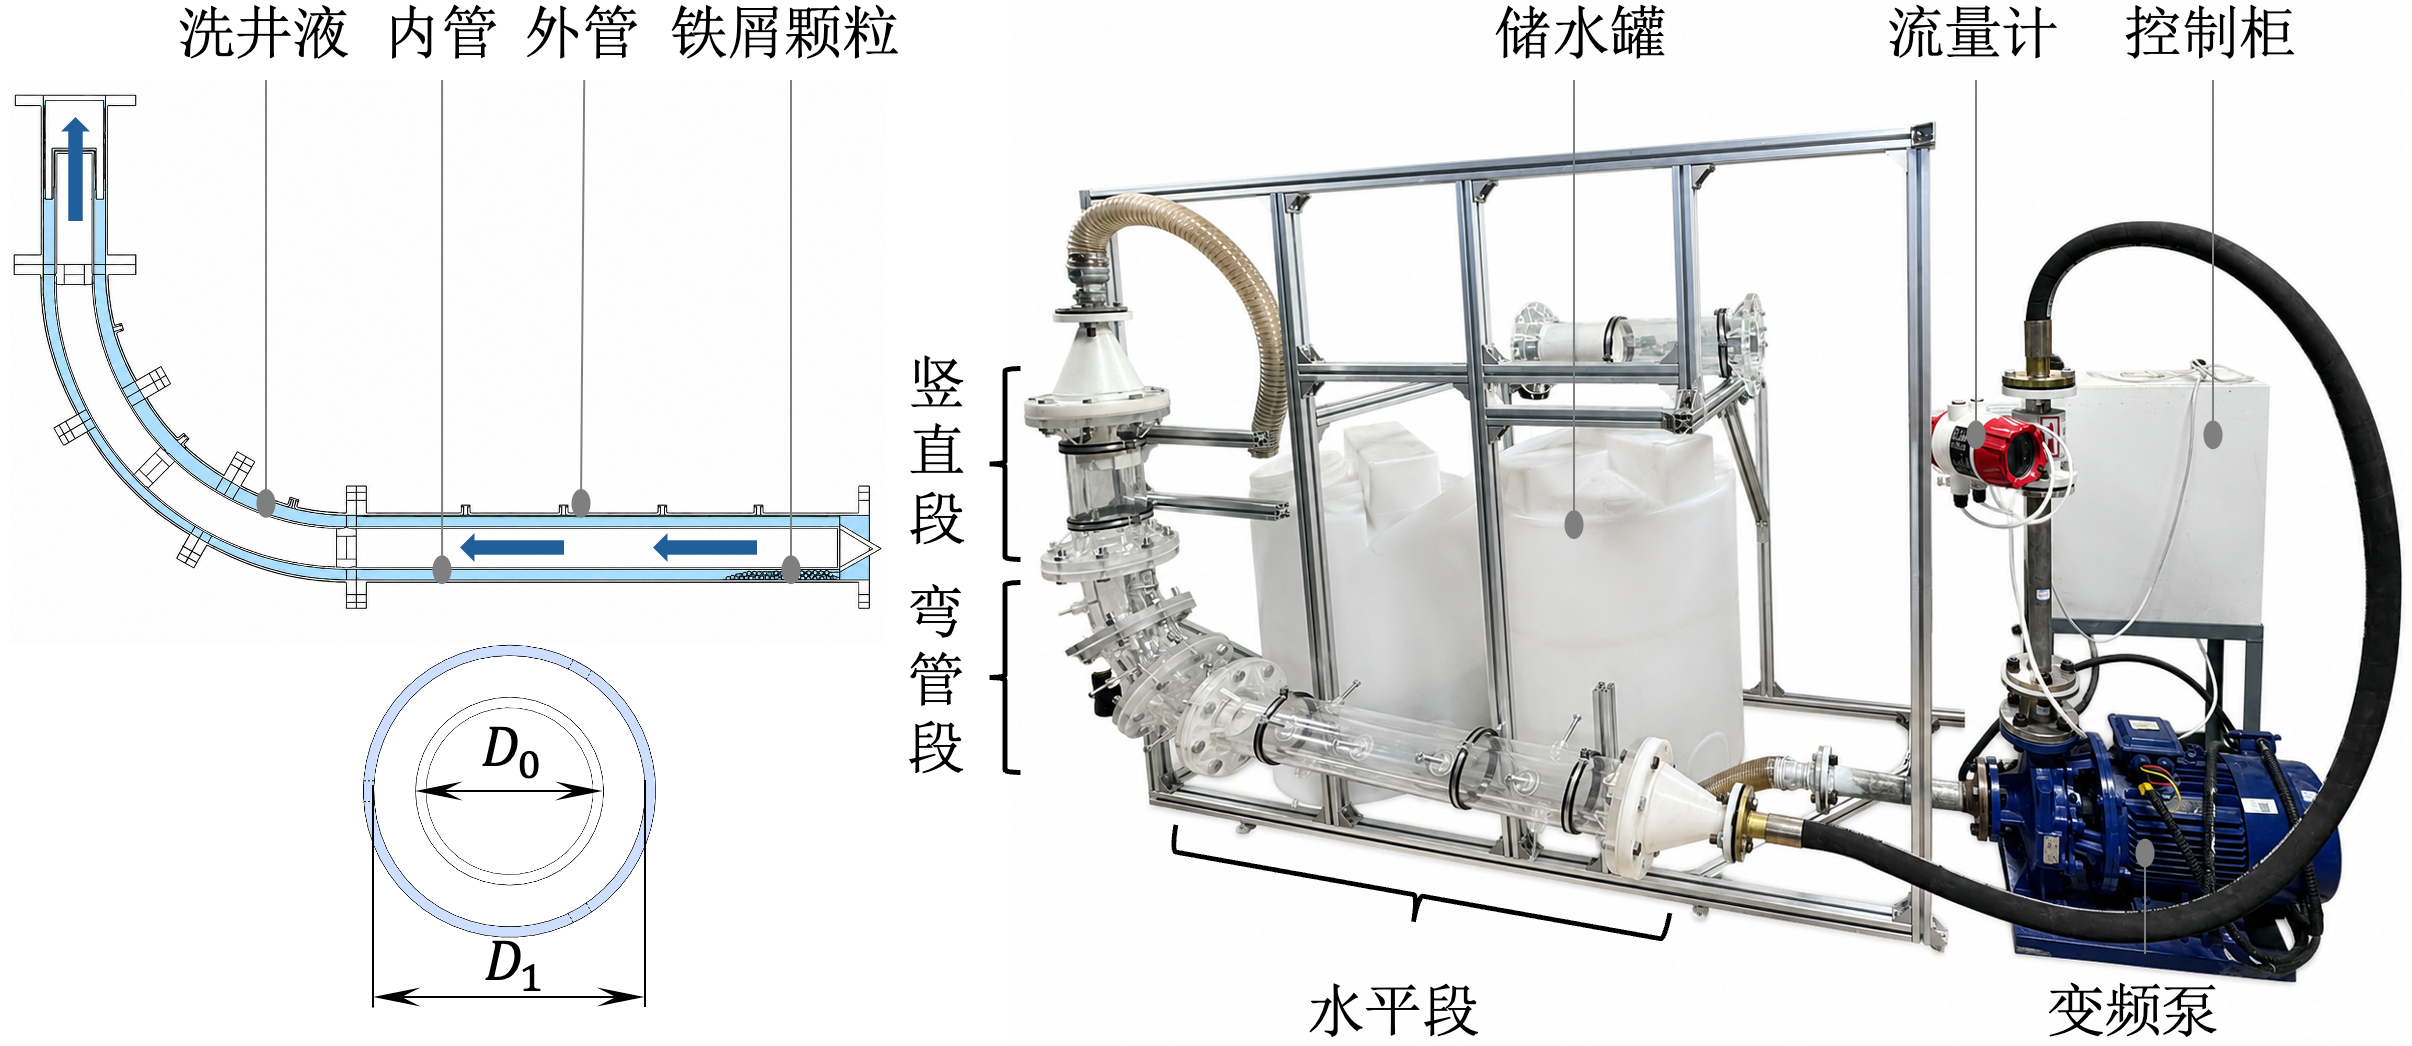
\includegraphics[width=1.\textwidth]{figure/chapter2/iron-washing-test-rig.png}
	\caption{研究洗井过程中铁屑运移规律的实验装置}
	\label{fig:iron_washing_test_rig}
\end{figure}

\subsection{实验结果及讨论}

水平段铁屑床的形态演变情况如图 \ref{fig:iron_bed_horizontal} 所示。随着泵流量$Q$的逐步增加，床层的宏观演化过程及流场特征表现出显著的阶段性规律。
当$Q=7.5\mathrm{m^3/h}$ 时，床层内的铁屑颗粒开始呈现运动趋势，部分颗粒自床层前缘起发生向后的位移，标志着床层由静止向流态化转变的初始阶段。当 $Q=10.00\mathrm{m^3/h}$ 时，铁屑床的宏观形态呈现出明显的非均匀拉伸特征：床层上部颗粒的运移距离显著大于下部颗粒。这种沿周向分布的运移差异表明，尽管设置了导流锥，但进口区域的流速分布不均现象尚未被完全消除，局部流场仍存在明显的梯度效应。
% TODO(核对): 正文 Q=7.5 m³/h 与图注 Q=7.85 m³/h 不一致，需以实测记录为准。
随着$Q=11.70\mathrm{m^3/h}$，铁屑床发生显著的宏观位移，其前缘已接近当前观测视野的边界。值得注意的是，在此高流量工况下，床层形态的演化反而表现出更高的均匀性与对称性。这一现象证实，随着流体向下游发展，环空区域的流速分布趋于均匀化，表明本实验系统对来流均匀性的整体控制质量良好，能够满足后续研究的流场要求。
\begin{figure}[htbp]
	\centering
	\subfloat[$Q=7.85\mathrm{m^3/h}$]{%
	
\includegraphics[width=.33\textwidth]{figure/chapter2/iron-bed-7dot85mperh.png}
	\label{fig:iron_bed_7dot85mperh}
	}
	%\vspace{1em}
	\subfloat[$Q=10.00\mathrm{m^3/h}$]{%
	
\includegraphics[width=.33\textwidth]{figure/chapter2/iron-bed-10dot00mperh.png}
	\label{fig:iron_bed_10dot00mperh}
	}
	\subfloat[$Q=11.70\mathrm{m^3/h}$]{%
	
\includegraphics[width=.33\textwidth]{figure/chapter2/iron-bed-11dot70mperh.png}
	\label{fig:iron_bed_11dot70_mperh}
	}
	\caption{水平段上铁屑床形态演变（铁屑床初始位置处俯视相机拍摄）}
	\label{fig:iron_bed_horizontal}
\end{figure}

随着流量的逐级提升，铁屑床表现出复杂的运动特征。即便在水平管段，颗粒床在达到临界启动流量后也非呈现简单的整体滑移模式，而是表现出“前缘不断剥蚀消失、后缘持续重塑堆积”的动态演化规律，且在整个运移过程中都有部分细小碎屑会受流体曳力作用从床层主体剥离，随主流场输运，导致铁屑床的质量递减。床层整体的运移速度随流速的增加而提升，但相对于环空的平均流速而言是较小值。弯管段与竖直段观测窗内的铁屑床形态演变分别如图\ref{fig:iron_bed_bend}和图\ref{fig:iron_bed_vertical}所示。
%后面的数据处理和速度为小值有直接关系，这里要扩展一下

\begin{figure}[htbp]
	\centering
	\subfloat[$Q=15.70\mathrm{m^3/h}$]{%
	
\includegraphics[width=.33\textwidth]{figure/chapter2/iron-bed-15dot70mperh.png}
	\label{fig:iron_bed_15dot70mperh}
	}
	%\vspace{1em}
	\subfloat[$Q=15.83\mathrm{m^3/h}$]{%
	
\includegraphics[width=.33\textwidth]{figure/chapter2/iron-bed-15dot83mperh.png}
	\label{fig:iron_bed_15dot83mperh}
	}
	\subfloat[$Q=17.44\mathrm{m^3/h}$]{%
	
\includegraphics[width=.33\textwidth]{figure/chapter2/iron-bed-17dot44mperh.png}
	\label{fig:iron_bed_17dot44_mperh}
	}
	\caption{弯管段铁屑床形态（弯管处正视相机拍摄）}
	\label{fig:iron_bed_bend}
\end{figure}

\begin{figure}[htbp]
	\centering
	\subfloat[铁屑床形态视频截图]{%
	
\includegraphics[width=.9\textwidth]{figure/chapter2/video-clip-theta-le-72-degree.png}
	\label{fig:video_clip_theta_le_72_degree}
	}
	\vspace{.5em}
	\subfloat[床面积提取结果]{%
	\begin{tikzpicture}
        % ================= 1. 放置完整的大图 =================
        % [name=img] 为图片命名，方便我们后续获取它的宽度
        % 替换 example-image 为你拼接好的那张完整大图的真实文件名（例如 full_image.png）
        \node[inner sep=0] (img) {
\includegraphics[width=.9\textwidth]{figure/chapter2/extraction-of-pack-area-theta-le-72-degree.png}};
        % ================= 2. 设置注释参数 =================
        % 这里的坐标是相对于大图的左下角 (0,0) 计算的
        \def\texty{-1.6} % 控制所有文字距离图片底部的垂直距离 (根据图片比例调整，负数表示向下偏移)
        % ================= 3. 在绝对坐标处添加注释 =================
        % 这里的 x 坐标（如 1.8, 3.6 等）是等间距的
        % 你需要根据你真实图片中子图的间距，手动微调这些 x 坐标
        \node at (-6.0, \texty) {${A^* = 1.00}$};
        \node at (-3., \texty) {${A^* = 0.64}$};
        \node at (0.0, \texty) {${A^* = 0.34}$};
        \node at (3., \texty) {${A^* = 0.05}$};
        \node at (6., \texty) {${A^* \approx 0.00}$};
    \end{tikzpicture}
	\label{fig:extraction_of_pack_area_theta_le_72_degree}
	}
	\caption{竖直段铁屑床形态（竖直管左视相机拍摄）}
	\label{fig:iron_bed_vertical}
\end{figure}

为精确量化这一过程，实验后通过视频帧分析提取了关键时间节点下的流量、位置及残留状态数据；特别是在弯管段的位置标定中，采用了实验视频与带刻度三维模型重叠匹配的方法，通过读取铁屑堆首尾端的刻度值，精确解算了床层质心的空间位置。实验观测表明，铁屑在弯管内的宏观迁移与进入竖直段后的流态化消散呈现出截然不同的动力学特征。前者主要体现为床层整体位置的时空演变，后者则侧重于固定堆积量的衰减过程。鉴于此，后续数据处理将针对这两个阶段分别选取特定的响应变量进行定量分析。

位置标定数据来自对原始视频的逐帧标定：在每个时刻识别铁屑床的头部与尾部，取二者角度的平均值作为床层中部位置，并记录对应的流量读数。标定共获得 $20$ 个有效点，如图\ref{fig:bed_position_VS_flow_rate_inclined_section}所示。角度范围覆盖 $\theta_c=0^{\circ}$-$72^{\circ}$，流量 $Q=14.25$-$18.09 \mathrm{m^3/h}$。其中 $\theta_c=51^{\circ}$-$63^{\circ}$区间因流量计读数在该时间段内出现异常波动，原始记录未采集到有效数据，这一区间在后续拟合中不参与计算，模型曲线由两侧的数据共同约束、连续给出。
$\theta_c>72^{\circ}$后，铁屑床主要进入竖直观察段并局部堆积，用弯管角度描述位置已不再适用，因此第二阶段改用视频提取的固定床可见面积作为响应量，用以描述床层的消散过程。

\begin{figure}[htbp]
	\centering
	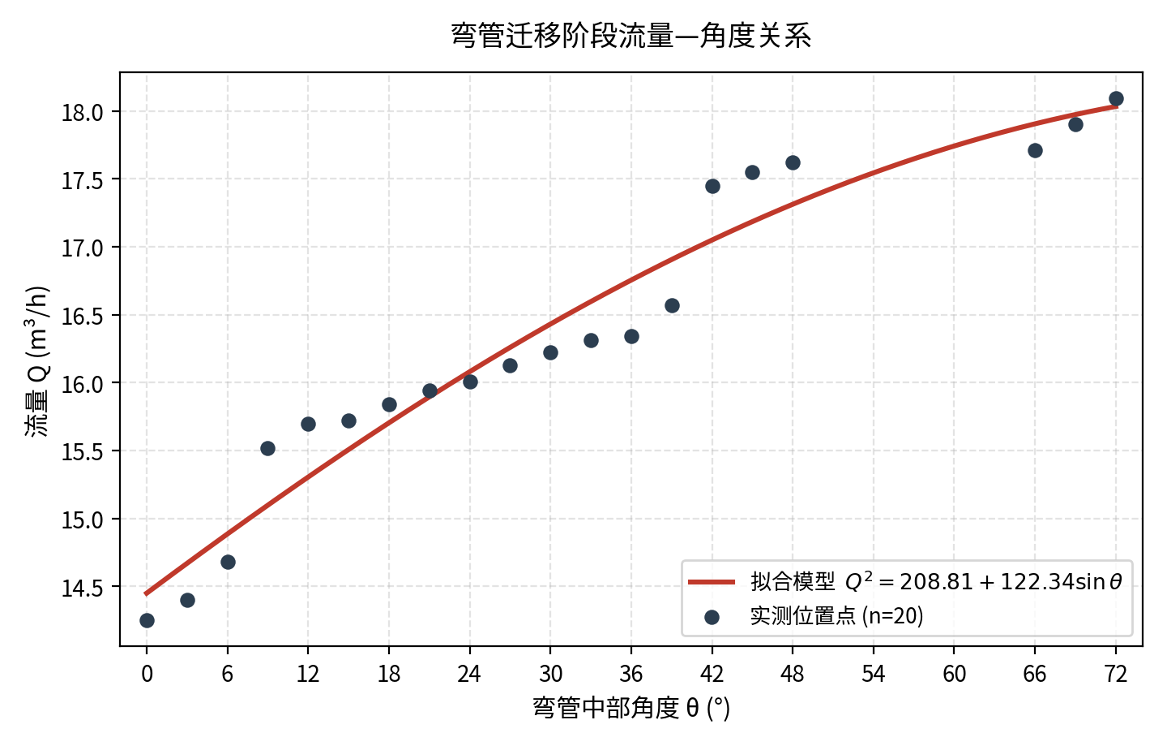
\includegraphics[width=1.0\textwidth]{figure/chapter2/bed-position-VS-flow-rate-inclined-section.png}
	\caption{弯管段铁屑床中部位置与流量的标定关系（$20$ 个有效标定点）}
	\label{fig:bed_position_VS_flow_rate_inclined_section}
\end{figure}
% TODO(待补): 给出各帧对应的流量/时刻与 A*(Q) 定量关系（第二阶段衰减模型），并与式\eqref{eq:bend_model}衔接。
在弯管迁移阶段，驱动铁屑床向前移动的是水流对床层的作用力，而阻碍其移动的主要是重力沿弯管切线方向的分量。参考直管水力学中过流量与壁面切应力的关系，流体作用力近似随流量的平方（$Q^2$）增长；重力切向分量则随弯管角度的正弦（$\sin\theta_c$）增长，在 $\theta_c=0^\circ$ 处最小、随角度增大而增大。将两者放在同一个力平衡框架下，可以得到如下候选形式
\begin{equation}
	Q^2(\theta_c) = A + B\cdot \sin\theta_c
	\label{eq:bend_candidate}
\end{equation}
式中，$A$、$B$为待定系数，量纲均为 $\mathrm{(m^3/h)^2}$。这一形式只用到了两个可从数据中辨识的组合参数，物理方向与力平衡机制一致，是后续候选模型比较的核心对象。

为避免主观选定单一形式，本文在同一数据集上比较了四类候选模型（见表\ref{tab:model_comparison}），统一以流量$Q$作为响应变量，通过决定系数$R^2$、均方根误差 RMSE、修正后的 AICc 以及留一交叉验证 RMSE（LOOCV RMSE）综合评估拟合优度与泛化能力：

\begin{table}[htbp]
    \centering
    \caption{候选模型拟合与交叉验证结果对比}
    \label{tab:model_comparison}
    \renewcommand{\arraystretch}{1.3}
    \begin{tabular}{llccccc}
        \toprule
        模型 & 函数形式 & 参数个数 & $R^2$ & RMSE & AICc & LOOCV RMSE \\
        \midrule
        重力分量力平衡 & $Q^2 = A + B\sin\theta_c$ & 2 & 0.942 & 0.267 & -48.15 & 0.294 \\
        二次多项式 & $Q = a + b\theta_c + c\theta_c^2$ & 3 & 0.943 & 0.265 & -45.63 & 0.302 \\
        经验幂函数 & $Q = Q_0 + c\theta_c^p$ & 3 & 0.945 & 0.261 & -46.26 & 0.313 \\
        线性 & $Q = a + b\theta_c$ & 2 & 0.911 & 0.331 & -39.50 & 0.376 \\
        \bottomrule
    \end{tabular}
\end{table}

二次多项式与经验幂函数的样本内 $R^2$ 略高于力平衡模型，但二者多用了一个自由参数，留一交叉验证误差反而没有改善，说明额外的自由度更多是在拟合噪声而非提升泛化能力。重力分量力平衡模型同时取得最低的 AICc 和最低的 LOOCV RMSE，且只用两个参数即达到与三参数模型相当的拟合优度，因此被选为最终模型。更高阶的分段拟合虽然可能进一步推高样本内 $R^2$ ，但会把 $\theta_c=51^\circ$～$63^\circ$ 的数据缺失和流量的局部波动误拟合成结构性拐点，不适合当前的数据规模。基于 $20$个有效位置点，最终确定的弯管迁移阶段模型为
\begin{equation}
	Q^2(\theta_c) = 208.57 + 122.69\sin \theta_c, \quad 0^\circ \le \theta_c \le 72^\circ
	\label{eq:bend_model}
\end{equation}
其中，基线项 $208.57$ 代表弯管起点附近床层接触、形状嵌锁与摩擦等综合阻力所对应的启动流量平方；系数 $122.69$ 代表重力切向分量随角度上升而增加的贡献。模型整体 $R^2$为 $0.942$，流量 RMSE 为 $0.267 \mathrm{m^3/h}$，LOOCV RMSE 为 $0.294 \mathrm{m^3/h}$。参数的 Bootstrap 95\% 置信区间为 $A \in [202.43, 216.75]$，$B \in [107.72, 134.89]$。由基线项换算得到的模型基准启动流量为 $Q_0 = 14.44 \mathrm{m^3/h}$（95\% 区间 $14.23-14.72 \mathrm{m^3/h}$），与实测中铁屑床到达弯管起始处的流量$14.25\mathrm{m^3/h}$ 十分接近，二者相互印证，说明模型在起点附近具有良好的物理合理性。
% TODO(待补): 补充 20 个标定点的数据表（或附录），以及 Bootstrap 重采样次数与置信区间方法说明。

因此，本文建立的是弯管迁移阶段的半经验模型与竖直段床层衰减的定量图像判据，用于描述本装置、本介质条件下铁屑床的启动、迁移与完全冲洗规律。


最终实验表明，随着泵流量增加，铁屑床经历由启动、沿弯管迁移、进入竖直段聚集并逐渐衰减，直至无可见颗粒的连续变化过程。在本实验条件下，约 $21.5\ \mathrm{m^3/h}$ 可作为最小观察性完全冲洗参考流量，约 $21.8\ \mathrm{m^3/h}$ 可作为较保守的无可见颗粒确认流量。
% TODO(待补): 说明 21.5 与 21.8 m³/h 的判定依据（无可见颗粒判据、观测窗分辨率），以及二者超出式\eqref{eq:bend_model}适用范围的说明。
需要说明的是，上述结论来源于本装置、本次约 $70\ \mathrm{g}$ 短小卷曲车削铁屑及当前流体条件下的一次连续升流量实验。由于流量与时间在实验中同步变化，且缺少多组恒定流量下的重复实验，所得模型与特征流量仅用于描述本台架条件下的实验规律；受数据规模与工况覆盖限制，尚不足以建立可外推至其他管径、流体或铁屑形态的完整输沙模型（如 Exner 输沙模型、Shields 临界起动模型或两层流模型），不宜直接外推至现场工况。

 % 全井筒模型
% --- 第三章 ---
\chapter{深度清洁工具设计}

井筒清洁是油气井作业的关键工序，其核心是清除井筒内的岩屑、砂粒、蜡垢、水垢、腐蚀产物等杂质，以保障井筒畅通、恢复产能、延长服役寿命，贯穿钻井、完井、修井及生产的全周期。现有井筒清洁技术功能单一、施工效率低，一体化与集成化程度低，难以满足油田开采降本增效的需求。为此，本研究通过理论研究丰富产品系列，形成了一套针对 9-5/8\inch 井筒的深度清洁工艺技术。本章针对该工艺技术的核心清洁工具，按照单工具工艺与工具组合工艺两部分展开：首先分别完成“三合一”脉冲式冲刮刷集成式井筒清洁工具、“四合一”通刮刷磁集成式井筒清洁工具、大容量强磁吸附工具、多功能过滤工具和可变径刮管工具的结构设计、理论计算与仿真校核，并给出各工具的使用与维护要求；然后结合不同井况要求给出上述工具的组合方式，以减少下钻趟数、提高作业效率。

\section[“三合一”脉冲式冲刮刷集成式井筒清洁工具设计]{“三合一”脉冲式冲刮刷集成式井筒清洁工具设计\protect\footnote{合同条款：5.1.3井筒高效清洁关键技术配套工具设计——（5）“三合一”脉冲式冲刮刷集成式井筒清洁工具设计}}\label{sec:design_of_3_in_1}
	\input{chapters/chapter3/part1-3in1-design.tex}
	\input{chapters/chapter3/part1-3in1-verification.tex}
	\input{chapters/chapter3/part1-3in1-hydraulic-model.tex}
	\input{chapters/chapter3/part1-3in1-setup-and-maintainance.tex}
\section{“四合一”通刮刷磁集成式井筒清洁工具设计}
	\input{chapters/chapter3/part2-4in1.tex}
	\input{chapters/chapter3/part2-4in1-scraper-performance.tex}
\section{大容量强磁吸附工具设计}
	\input{chapters/chapter3/part3-magntictool.tex}
\section{多功能过滤工具设计}
	\input{chapters/chapter3/part4-filter.tex}
\section[可变径刮管工具设计]{可变径刮管工具设计\protect\footnote{合同条款：5.1.3井筒高效清洁关键技术配套工具设计——（4）可变径刮管工具设计}}
	\subsection{工具总体结构设计}

GGQ95 型可变径套管刮管器用于通过 7\inch 套管后，清除 9-5/8\inch 套管内壁上的残余水泥、泥块、轧制过程中产生的毛刺与鳞片、管内防砂射孔时镶在管壁上的射孔弹、生产井套管上的铁锈与水垢以及硬石蜡等影响正常施工作业的杂物。其结构如图~\ref{fig:variable_scrapter_structure}所示，可变径套管刮削器由上接头、旋转连杆座、连杆、刮刀、芯轴、复位总成、工作活塞、工作弹簧、下接头、节流喷嘴、中间外筒、中间芯轴、激活球座、钢球以及标准件、密封件等零件组成。刮刀采用两组 5 瓣圆周错位排布，覆盖 9-5/8\inch 套管内径圆周 360° 方向。

该工具的工作原理为：投球后激活球座下行，建立活塞腔与工具水眼流道，水眼内的液压力推动工作活塞并迫使工作弹簧上行，在连杆机构的作用下刮刀张开、贴紧套管内壁；随后上提、下放管柱即可实现刮刀对套管内壁的刮削清洁。工具的上下接头分别连接管柱，并通过芯轴连接，可传递扭矩和提拉、下放载荷；旋转连杆座可迫使整组刮刀绕工具自由旋转，当套管内壁变形或通过性较差时，刮刀可绕工具旋转错位通过。该工具的技术参数见表~\ref{tab:ggq95}。

\begin{figure}[htbp]
	\centering
	
\includegraphics[width=1.\textwidth]{figure/chapter3/part5/variable-scrapter-structure.png}
	\caption{可变径刮管器结构示意图}
	\label{fig:variable_scrapter_structure}
\end{figure}

\begin{table}[htbp]
    \centering
    \caption{GGQ95型可变径套管刮管器技术参数}
    \label{tab:ggq95}
    \renewcommand{\arraystretch}{1.2} % 适当增加行高，提升阅读体验
    \small % 调整整体字号，适应表格宽度
    \begin{tabular}{ccccccc}
        \toprule
        型号 & \begin{tabular}[c]{@{}c@{}}本体最大外径\\(mm)\end{tabular} & \begin{tabular}[c]{@{}c@{}}刮刀收回最小外径\\(mm)\end{tabular} & \begin{tabular}[c]{@{}c@{}}刮刀最大外径\\(mm)\end{tabular} & \begin{tabular}[c]{@{}c@{}}水眼\\(mm)\end{tabular} & \begin{tabular}[c]{@{}c@{}}总长\\(mm)\end{tabular} & \begin{tabular}[c]{@{}c@{}}接头扣\\(API)\end{tabular} \\
        \midrule
        GGQ95 & 140 & 136 & 229+ & 38.1 & 2965 & NC38 \\
        \bottomrule
    \end{tabular}
\end{table}


\subsection[可变径刮管工具设计计算与校核]{可变径刮管工具设计计算与校核\protect\footnote{合同条款：5.2.1.3井筒高效清洁关键技术配套工具设计——（4）可变径刮管工具：抗拉$>=100\mathrm{T}$，抗扭$>17\,\mathrm{kN}\cdot\mathrm{m}$}}


\subsubsection{主要受力件的螺纹强度校核}

9-5/8\inch 可变径刮壁器的主要受力件为刮刀芯轴，其主要受力螺纹为 $\mathrm{Tr}\,65 \times 4-8e$，危险截面即位于该螺纹的根部。

螺纹牙的剪切强度按下式计算：
\begin{align}
    F_{\max} &= [\tau] \cdot k_z \cdot \pi \cdot d_1 \cdot b \cdot z \cdot 10^{-3} \\
    [\tau] &= \frac{\sigma_s}{n}
\end{align}
式中，$F_{\max}$---工具最大拉力，kN；

$[\tau]$---螺纹牙的许用剪切强度，MPa；

$k_z$---螺纹各圈的载荷不均系数，根据《机械设计手册》螺纹连接（紧固件连接）部分中螺纹牙的剪切强度计算及各圈螺纹载荷分配的规定\cite{ref26}，取 $k_z = 0.56$；

$d_1$---螺纹底径，mm；

$b$---螺纹牙根宽度，mm；

$z$---旋合圈数；

$\sigma_s$---材料最小屈服强度，取 1068 MPa；

$n$---安全系数，根据《机械设计手册》螺纹连接部分中螺纹牙强度校核的安全系数取值规定\cite{ref26}，取 $n = 2.5$。

将 $\mathrm{Tr}\,65 \times 4-8e$ 螺纹的相关参数代入，计算得：
\begin{align}
    F_{\max} &= [\tau] \cdot k_z \cdot \pi \cdot d_1 \cdot b \cdot z \cdot 10^{-3} \\
             &= 427.2 \times 0.56 \times 3.14 \times 62 \times 2.6 \times 23.5 \times 10^{-3} \\
             &= 2845.65\,\mathrm{kN} \\
             &> 1000\,\mathrm{kN}
\end{align}

计算结果表明，螺纹牙的剪切强度满足设计要求。


\subsubsection{主要受力件的零件抗拉强度校核}

9-5/8\inch 可变径刮壁器的主要受力件为刮刀芯轴和芯轴连接筒，两者的抗拉危险截面分别为刮刀芯轴小螺纹 $\mathrm{Tr}\,65 \times 4-8e$ 螺纹根部和芯轴连接筒内螺纹 $\mathrm{Tr}\,65 \times 4-8H$ 螺纹根部。

抗拉强度按下式计算：
\begin{equation}
    F_{\max} = \frac{\pi \cdot (D^2 - d^2) \cdot \sigma_s}{4 \cdot n} \times 10^{-3}
\end{equation}
式中，$F_{\max}$---工具最大拉力，kN；

$D$---危险截面外径，mm；

$d$---危险截面内径，mm；

$\sigma_s$---材料最小屈服强度，取 1068 MPa；

$n$---安全系数，取 $n = 1.5$。

（1）刮刀芯轴危险截面最大抗拉计算
\begin{align}
    F_{\max} &= \frac{\pi \cdot (D^2 - d^2) \cdot \sigma_s}{4 \cdot n} \times 10^{-3}
             = \frac{3.14 \times (62^2 - 38.1^2) \times 1068}{4 \times 1.5} \times 10^{-3} \\
             &= 1337.15\,\mathrm{kN} > 1000\,\mathrm{kN}
\end{align}
满足设计要求。

（2）芯轴连接筒危险截面最大抗拉计算
\begin{align}
    F_{\max} &= \frac{\pi \cdot (D^2 - d^2) \cdot \sigma_s}{4 \cdot n} \times 10^{-3}
             = \frac{3.14 \times (80^2 - 66^2) \times 1068}{4 \times 1.5} \times 10^{-3} \\
             &= 1142.43\,\mathrm{kN} > 1000\,\mathrm{kN}
\end{align}
满足设计要求。


\subsubsection{主要受力件的零件抗扭强度校核}

9-5/8\inch 可变径刮壁器的主要受力件为刮刀芯轴和芯轴连接筒，其抗扭危险截面与抗拉校核相同，分别位于刮刀芯轴小螺纹 $\mathrm{Tr}\,65 \times 4-8e$ 螺纹根部和芯轴连接筒内螺纹 $\mathrm{Tr}\,65 \times 4-8H$ 螺纹根部。

抗扭强度按下式计算：
\begin{align*}
    \tau &= \frac{16 \cdot D \cdot T_{\max}}{\pi \cdot (D^4 - d^4)} \times 10^{6} \\
    T_{\max} &= \frac{[\tau] \cdot \pi \cdot (D^4 - d^4)}{16 \cdot D} \times 10^{-6} \\
    [\tau] &= n \cdot \sigma_s = 0.66 \times 1068\,\mathrm{MPa} = 704.88\,\mathrm{MPa}
\end{align*}
式中，$T_{\max}$---工具最大扭矩，$\mathrm{kN}\cdot\mathrm{m}$；

$\tau$---危险截面的切应力，MPa；

$[\tau]$---材料许用切应力，MPa；

$\sigma_s$---材料屈服强度，MPa；

$D$---危险截面外径，mm；

$d$---危险截面内径，mm；

$n$---许用切应力与许用拉应力之比，根据《机械设计手册》零件强度校核中许用应力折减系数的取值规定\cite{ref26}，取 $n = 0.66$。

（1）刮刀芯轴危险截面最大抗扭计算
\begin{align}
    T_{\max} &= \frac{[\tau] \cdot \pi \cdot (D^4 - d^4)}{16 \cdot D} \times 10^{-6}
             = \frac{704.88 \times 3.14 \times (62^4 - 38.1^4)}{16 \times 62} \times 10^{-6} \\
             &= 28.27\,\mathrm{kN}\cdot\mathrm{m} > 17\,\mathrm{kN}\cdot\mathrm{m}
\end{align}
满足设计要求。

（2）芯轴连接筒危险截面最大抗扭计算
\begin{align}
    T_{\max} &= \frac{[\tau] \cdot \pi \cdot (D^4 - d^4)}{16 \cdot D} \times 10^{-6}
             = \frac{704.88 \times 3.14 \times (80^4 - 66^4)}{16 \times 80} \times 10^{-6} \\
             &= 38.02\,\mathrm{kN}\cdot\mathrm{m} > 17\,\mathrm{kN}\cdot\mathrm{m}
\end{align}
满足设计要求。


\subsubsection{球座剪钉剪切力与节流泵压计算}

9-5/8\inch 可变径刮壁器需要投球后憋压将球座剪钉剪断，迫使球座下移建立压力通道才能开始工作，因此剪钉的剪断力和投球后球座处的憋压压力是激活工具的重要参数。

刮壁器的球座圆周设计 3 组剪钉参与剪切，剪钉选用 45 号非调质料制作，则工具激活所需的推力为：
\begin{equation}
    \begin{aligned}
        F_s \ge [\tau] \cdot A = 0.8 \times [\sigma] \times 3 \times (\pi \cdot R^2) &= 0.8 \times 450 \times 3 \times 3.14 \times 4^2 \\
        &= 54259.2\,\mathrm{N}
    \end{aligned}
\end{equation}
式中，$F_s$---工具激活所需的最小推力，N；

$[\tau]$---材料许用剪应力，塑性材料取 $0.6[\sigma]$、脆性材料取 $0.8[\sigma]$；

$A$---单个剪钉的剪切面积，$\mathrm{mm}^2$；

$R$---单个剪钉的半径，mm。

刮壁器投入钢球后球座流道被堵塞，井口泵压直接作用在球座上，根据上述计算所得的最小推力 $F_s$，可计算出激活工具所需的最小泵压 $P_0$：
\begin{equation}
    P_0 \ge \frac{F_s}{A_q} = \frac{F_s}{\pi \cdot \left(\frac{d}{2}\right)^2} = \frac{54259.2}{3.14 \times \left(\frac{45}{2}\right)^2} = 34.12\,\mathrm{MPa}
\end{equation}
式中，$P_0$---激活工具所需的最小泵压，MPa；

$A_q$---球座承压面积，$\mathrm{mm}^2$；

$d$---球座承压面直径，取 45 mm。

计算表明，当泵压不小于 $34.12\,\mathrm{MPa}$ 时，工具可以被激活。


\subsubsection{节流喷嘴的尺寸和节流压力关系}

刮壁器激活后流道建立，工具底部的节流喷嘴形成的节流压差为工具提供工作压力 $\Delta P \le 4\,\mathrm{MPa}$，故需要计算节流喷嘴的尺寸与节流压力的关系。

由公式：
\begin{equation}
    \Delta P \le \frac{827 \cdot \rho \cdot Q^2}{C^2 \cdot d_e^4}
\end{equation}

推算喷嘴最小直径为：
\begin{equation}
    d_e \ge \sqrt[4]{\frac{827 \cdot \rho \cdot Q^2}{C^2 \cdot \Delta P}} = \sqrt[4]{\frac{827 \times 1.1 \times 40^2}{0.96^2 \times 4}} = 25.06\,\mathrm{mm}
\end{equation}
式中，$d_e$---喷嘴节流孔最小直径，mm；

$\Delta P$---刮壁器最大节流压力（即最大节流工作压差），MPa；

$\rho$---钻井液密度，$1.1\,\mathrm{g/cm^3}$；

$Q$---工作时泵排量，暂定值为 $40\,\mathrm{L/s}$；

$C$---流量系数，无因次，取 $0.95 \sim 0.98$。


\subsubsection{连杆销抗剪切强度计算}

9-5/8\inch 可变径刮壁器在激活后的工作过程中，刮壁作业所承受的冲击载荷由连杆铰链销承受，故有必要计算连杆销的抗剪切强度。假定刮壁器作业时受到的最大轴向力为工具最大抗拉力，即 $F_{\max} = 1000\,\mathrm{kN}$；销钉材料选用 M35 热后料，$[\sigma] \ge 1300\,\mathrm{MPa}$；销钉设计最小直径为：

由切应力公式
\begin{equation}
    \tau = \frac{F_{\max}}{A} = \frac{F_{\max}}{20 \cdot A_0} = \frac{F_{\max}}{\pi \cdot 20 \cdot \left(\frac{d}{2}\right)^2} \le [\tau]
\end{equation}
式中，$[\tau]$---材料许用剪应力，MPa，塑性材料取 $0.6[\sigma]$、脆性材料取 $0.8[\sigma]$，本例取 $1040\,\mathrm{MPa}$；

$A$---单个连杆销的总剪切面积，每个连杆销有两个剪切面积，故 $A = 2 \times 2A_0 \times 5$；

$d$---连杆销的最小直径，mm。

可得
\begin{equation}
    d \ge 2\sqrt{\frac{F_{\max}}{20 \cdot \pi \cdot [\tau]}} = 2\sqrt{\frac{1.0 \times 10^{6}}{20 \times 3.14 \times 1040}} = 7.825\,\mathrm{mm}
\end{equation}

设计连杆销直径 $d = 8\,\mathrm{mm}$，满足设计要求。


\subsubsection{主要受力件仿真校核}

主要受力件为刮刀芯轴和芯轴连接筒，危险截面出现在螺纹根部，有限元仿真结果如图~\ref{fig:FEA_inner_pipe_variable}所示。刮刀芯轴的最大拉应力为 850 MPa，小于设计要求；最大切应力为 1600 MPa，出现在变径处，但范围极小，属于应力集中导致的局部小尺度高应力，不会引发整体塑性变形，强度满足设计要求。

\begin{figure}[htbp]
	\centering
	\subfloat[可变径刮管器心轴]{%
	
\includegraphics[width=0.7\textwidth]{figure/chapter3/part5/inner-pipe.png}
	}
	\hfill
	\subfloat[抗拉强度分析]{%
	
\includegraphics[width=0.4\textwidth]{figure/chapter3/part5/tensile-strength.png}
	}
	\vspace{1em}
	\subfloat[抗扭强度分析]{%
	
\includegraphics[width=0.3\textwidth]{figure/chapter3/part5/torsional-strength.png}
	}
	\caption{可变径刮管工具薄弱零件强度有限元分析}
	\label{fig:FEA_inner_pipe_variable}
\end{figure}


\subsection{拆装步骤}

工具入井后到达管子站进行保养前，需冲洗外表面，并准备好内六角扳手、起子、扳手等拆卸工具。

(1) 工具冲洗干净后，将上、下接头的 M16 螺钉拆卸，取出内部的防掉钢珠；取出下接头喷嘴；如下图箭头所示位置。

\begin{figure}[htbp]
\centering
	
\includegraphics[width=1.\textwidth]{figure/chapter3/part5/unsetup/ball.png}
\end{figure}

(2) 拆卸上、下接头的防松螺钉后，分别反转拆卸上、下接头；如下图所示位置。

\begin{figure}[htbp]
\centering
	
\includegraphics[width=1.\textwidth]{figure/chapter3/part5/unsetup/unsetup-satefy-screw.png}
	\vspace{1em}
	
\includegraphics[width=1.\textwidth]{figure/chapter3/part5/unsetup/unsetup-two-subs.png}
\end{figure}

(3) 用起子、扳手取下连杆座、连杆、刮刀等之间的铰链销、防掉螺钉等标准件后，依次拆卸旋转连杆座、连杆、刮刀等零件；如下图所示。

\begin{figure}[htbp]
\centering
	
\includegraphics[width=1.\textwidth]{figure/chapter3/part5/unsetup/unsetup-fasten-parts.png}
\end{figure}

(4) 拆卸各部位的锁紧螺钉、铰链销、防掉螺钉等零件。

(5) 拆卸两头的旋转连杆座。

\begin{figure}[h]
\centering
	
\includegraphics[width=1.\textwidth]{figure/chapter3/part5/unsetup/rotary-lever-set.png}
\end{figure}

(6) 拆卸两头的连杆、刮刀等零件。

\begin{figure}[htbp]
\centering
	
\includegraphics[width=1.\textwidth]{figure/chapter3/part5/unsetup/end-links.png}
	
\includegraphics[width=1.\textwidth]{figure/chapter3/part5/unsetup/unsetup-scraper.png}
	
\includegraphics[width=1.\textwidth]{figure/chapter3/part5/unsetup/left-links.png}
\end{figure}

(7) 分别反转拆卸两头的芯轴，从下部取出激活球座和钢球，如下图所示。

\begin{figure}[htbp]
\centering
	
\includegraphics[width=1.\textwidth]{figure/chapter3/part5/unsetup/unsetup-inner-pipe.png}
	
\includegraphics[width=1.\textwidth]{figure/chapter3/part5/unsetup/unsetup-ball-and-seat.png}
\end{figure}

(8) 夹紧中间外筒方向旋转复位总成，分别取出上、下两头的复位总成，然后依次对复位总成进行拆解，如下图所示。

\begin{figure}[htbp]
\centering
	
\includegraphics[width=1.\textwidth]{figure/chapter3/part5/unsetup/reseting-assembly.png}
	
\includegraphics[width=1.\textwidth]{figure/chapter3/part5/unsetup/resetting-assembly-unsetup.png}
\end{figure}

(9) 取出中间筒体和中间芯轴的限位钢球，随后取下中间芯轴、弹簧、活塞、活塞限位套等零件；最后拆卸各零件上的密封圈，即拆卸完毕。

(10) 拆卸中间筒体和中间芯轴的钢球堵和限位钢球。

\begin{figure}[htbp]
\centering
	
\includegraphics[width=1.\textwidth]{figure/chapter3/part5/unsetup/middle-body-inner-pipe-ball.png}
\end{figure}

(11) 拆卸中间芯轴，固定中间筒体后从任意一头抽出中间芯轴即可。

\begin{figure}[htbp]
\centering
	
\includegraphics[width=1.\textwidth]{figure/chapter3/part5/unsetup/middle-inner-pipe-unsetup.png}
\end{figure}

(12) 按下图所示方向，分别从两头拆卸活塞、工作弹簧、活塞限位套等零件。

\begin{figure}[htbp]
\centering
	
\includegraphics[width=1.\textwidth]{figure/chapter3/part5/unsetup/piston-spring-limiter.png}
\end{figure}

(13) 装配步骤与拆卸步骤相反，装配过程中需要注意不要损伤密封面、螺纹牙形等配合处，密封面和螺纹组装前要求涂抹润滑油。

工具的易损件及配件清单见表~\ref{tab:parts_list}。

\begin{table}[htbp]
    \centering
    \caption{易损件及配件清单表}
    \label{tab:parts_list}
    \small % 代号较长，缩小字号以适应表格宽度
    \setlength{\tabcolsep}{4pt} % 减小列间距，避免超出正文版心
    \renewcommand{\arraystretch}{1.5} % 调整行间距，使表格不拥挤
    \begin{tabular}{cccc}
        \toprule
        \textbf{序号} & \textbf{代号} & \textbf{名称} & \textbf{单套数量} \\
        \midrule
        1  & 2-223 PAEKE FKM                      & O 形圈                 & 1   \\
        2  & GB/T308-2002 $\phi 30$               & 钢球 30                & 1   \\
        3  & ON 0800 052 00110 D （PARKE）        & 双作用格莱圈           & 2   \\
        4  & 2-243 PAEKE FKM                      & O 形圈                 & 2   \\
        5  & 2-222 PAEKE FKM                      & O 形圈                 & 2   \\
        6  & 2-229 PAEKE FKM                      & O 形圈                 & 2   \\
        7  & 2-140 PAEKE FKM                      & O 形圈                 & 2   \\
        8  & 2.62*62 GB/T1235                     & O 形圈                 & 2   \\
        9  & GB/T 77-2007                         & 内六角平端紧定螺钉 M8$\times$20  & 10  \\
        10 & GB/T 80-2007                         & 内六角凹端紧定螺钉 M8$\times$30  & 8   \\
        11 & GB/T 80-2007                         & 内六角凹端紧定螺钉 M8$\times$10  & 8   \\
        12 & GB/T 79-2007                         & 内六角圆柱端紧定螺钉 M10$\times$30 & 10  \\
        13 & GB/T 77-2007                         & 内六角平端紧定螺钉 M8$\times$8   & 8   \\
        14 & $\phi 25$ 喷嘴                       & 节流喷嘴               & 1   \\
        15 & G98Cr18 12 G40 $\pm 0$ GB/T 308      & $\phi 12$ 钢球         & 100 \\
        16 & GB/T 80-2007                         & 内六角凹端紧定螺钉 M5$\times$12  & 40  \\
        17 & GB/T 77-2007                         & 内六角平端紧定螺钉 M16$\times$16 & 2   \\
        18 & GB/T 77-2007                         & 内六角平端紧定螺钉 M10$\times$35 & 20  \\
        19 & GGQ95-19                             & 工作弹簧               & 2   \\
        20 & GGQ95-18                             & 复位弹簧               & 2   \\
        21 & GGQ95-17                             & 密封堵                 & 2   \\
        22 & GGQ95-16                             & 丝堵                   & 2   \\
        23 & GGQ95-7                              & 刮刀铰链销             & 20  \\
        24 & GGQ95-6                              & 59BPF 刮刀             & 10  \\
        25 & GGQ95-5                              & 活动铰链销             & 20  \\
        \bottomrule
    \end{tabular}
\end{table}


\subsection{操作方式}

\subsubsection{下井前准备}
\begin{itemize}
	\item 了解井况，确定套管规格和深度等基本信息；
	\item 选配适合套管规格的刮刀；
	\item 本可变径刮管器应与 7\inch 及以上其它刮管器配合使用；
	\item 确定刮管工艺，了解泵压和排量，并根据图~\ref{fig:pressure_decrease_with_Q_size}所示不同排量下喷嘴尺寸与压降的关系选装合适的喷嘴及剪钉。
\end{itemize}

\begin{figure}[htbp]
	\centering
	\subfloat[10L/s]{%
	
\includegraphics[width=0.4\textwidth]{figure/chapter3/part5/10LperSec.png}
	}
	%\hfill
	\subfloat[20L/s]{%
	
\includegraphics[width=0.4\textwidth]{figure/chapter3/part5/20LperSec.png}
	}
	\vspace{1em}
	\subfloat[30L/s]{%
	
\includegraphics[width=0.4\textwidth]{figure/chapter3/part5/30LperSec.png}
	}
	\subfloat[40L/s]{%
	
\includegraphics[width=0.4\textwidth]{figure/chapter3/part5/40LperSec.png}
	}
	\caption{喷嘴压降与排量、喷嘴尺寸之间的关系}
	\label{fig:pressure_decrease_with_Q_size}
\end{figure}

\subsubsection{操作}
\begin{itemize}
	\item 下井前按照作业要求依次连接好管柱，刮管器前端需接与套管规格对应的扶正器；推荐管柱组合为：通井钻头 $+$ 扶正器 $+$ 7\inch 刮管器 $+$ 可变径刮管器 $+$（选装其它套管清洁工具）$+$ 上部钻柱。
	\item 接上可变径刮管器后，夹紧下接头、大钳打上接头，拧紧刮管器各螺纹，井口以开泵压力 $\le 20 \pm 5\,\mathrm{MPa}$、排量 $\le 10\,\mathrm{L/s}$ 进行试循环，时间 $1 \sim 5\,\mathrm{min}$。
	\item 待循环正常并确定刮刀未弹出本体后，慢慢旋转下放工具，并进行其它钻磨、完井、试油、测试、刮小规格套管等作业。
	\item 当小规格套管刮管作业完成后，将可变径刮管器提升至 9-5/8\inch 套管所需的井深位置，投入钢球，开泵打压激活刮刀张开，启动作业；
	\item 刮管器打开压力 $=$ 静液柱压力 $+$ 泵压（绝对压力），即泵压 $\ge$ 绝对压力 $-$ 静液柱压力。
	\item 激活判定：投入钢球后观察泵压，若泵压上升过程中突然下降，说明可变径刮管器已启动；随后停泵，按工具入井前选定的喷嘴尺寸所要求的泵压和排量稳定循环，同时通过上提、下放工具进行 9-5/8\inch 套管的刮管作业。
	\item 刮管作业时观察指重表无任何显示，即下放悬重不降、上提悬重不升，表明已刮削干净。
\end{itemize}

\subsubsection{注意事项}
\begin{itemize}
	\item 工具与管柱的连接扣必须拧紧。
	\item 两组刮刀的螺旋升角应保持同方向。
	\item 可变径刮管器在下井过程中如遇阻，应慢慢旋转几圈后再下放。
	\item 刮管作业过程中，必须始终保持钻井液循环畅通。
\end{itemize}

\subsection{维护与保养}
\begin{itemize}
	\item 出井后应清洗干净，并检查各零件，如弹簧失效必须更换。各螺纹涂螺纹脂，各零件涂油，存放在阴干处。
	\item 每次作业后，都应将工具完全拆开并清洗，更换所有 O 形圈和损坏的弹簧，检查刮管器本体上的内套是否粘接牢固。用肉眼检查所有的密封面和接头丝扣是否损坏，若发现有损坏的零件都应更换，这些损坏的零件对工具的可靠性会产生不利的影响。
	\item 在拆卸、保养前，应准备好正确、有效的装配图和工具保养维护说明书及工具维护保养单。
	\item 对高温井作业以及有酸及硫化氢存在的修井作业，应提前更换相应耐腐蚀、耐高温的密封件和配件。
	\item 有关该工具使用和维护保养的其他任何问题，请与我校联系。
\end{itemize}

	
% === 【修改】GB/T 7714-2015 参考文献 ===
\clearpage % 参考文献另起一页
\addcontentsline{toc}{chapter}{参考文献} % 将参考文献加入目录

\bibliographystyle{gbt7714-numerical} % 采用顺序编码制（结题报告常用）
\begin{thebibliography}{99}

\bibitem{ref1} % 期刊文章示例
\textcolor{red}{Wicks, M. Transport of Solids at Low Concentration in Horizontal Pipes. In Advances in Solid–Liquid Flow in Pipes and Its Application; 1971; pp. 101–124.}

\bibitem{ref2} % 期刊文章示例
\textcolor{red}{King, M.J.S.; Fairhurst, C.P.; and Hill, T.J. Solids Transport in Multiphase Flows—Application to High-Viscosity Systems. ASME. J. Energy Resour. Technol. 2001, 123, 200–204. }


\bibitem{ref3} % 期刊文章示例
\textcolor{red}{李明忠, 王卫阳, 何岩峰, 等. 垂直井筒携砂规律研究[J]. 石油大学学报: 自然科学版, 2000, 24(2): 4.}


\bibitem{ref4} % 期刊文章示例
\textcolor{red}{李明忠, 王卫阳, 赵国景. 垂直井筒井液携砂流动规律研究及其在油井生产中的应用[J]. 实验力学, 2002(03): 385-392.}


\bibitem{ref5} % 期刊文章示例
\textcolor{red}{王治中, 邓金根, 孙福街, 等. 井筒砂粒运移规律室内模拟实验研究[J]. 石油学报, 2006(04): 130-132+138.}


\bibitem{ref6} % 期刊文章示例
\textcolor{red}{苏健鹏. 水平-竖直集气管道砂沉积规律与携砂特性研究[D]. 青岛: 中国石油大学(华东), 2019.}


\bibitem{ref7} % 期刊文章示例
\textcolor{red}{Danielson, T.J. Danielson, Thomas J. Sand Transport Modeling in Multiphase Pipelines. In Proceedings of the Offshore Technology Conference, Houston, Texas, USA, 30 April-3 May 2007. }


\bibitem{ref8} % 期刊文章示例
\textcolor{red}{Zeinali, H. Effect of Near-Wall Turbulence on Selective Removal of Particles from Sand Beds Deposited in Pipelines. Ph.D. University of Alberta, Edmonton, Alberta, AB, Canada, 2012.}


\bibitem{ref9} % 期刊文章示例
\textcolor{red}{侯学文. 水平井冲砂作业砂液两相流动与沉降特性研究[D]. 湖北: 长江大学, 2024.}


\bibitem{ref10} % 期刊文章示例
\textcolor{red}{Archibong-Eso, A.; Aliyu, A.M.; Yan, W.; Okeke, N.E.; Baba, Y.D.; Fajemidupe, O.; Yeung, H. Experimental Study on Sand Transport Characteristics in Horizontal and Inclined Two-Phase Solid–Liquid Pipe Flow. J. Pipeline Syst. Eng. Pract. 2020, 11, 04019050.}


\bibitem{ref11} % 期刊文章示例
\textcolor{red}{Doan, Q.T.; Doan, L.T.; Farouq Ali, S.M.; Oguztoreli, M. Sand Deposition inside a Horizontal Well—A Simulation Approach. J. Can. Pet. Technol. 2000, 39(10).}


\bibitem{ref12} % 期刊文章示例
\textcolor{red}{Najmi, K. Particle Transport in Single-Phase and Multiphase Horizontal Pipes with Emphasis on the Effect of Viscosity; The University of Tulsa,Tulsa, Oklahoma, USA, 2015.}


\bibitem{ref13} % 期刊文章示例
\textcolor{red}{Piroozian, A.; Ismail, I.; Yaacob, Z.; Babakhani, P; Ismail, A. Impact of Drilling Fluid Viscosity, Velocity and Hole Inclination on Cuttings Transport in Horizontal and Highly Deviated Wells. J. Pet. Explor. Prod. Technol 2. 2012 :149-456.}


\bibitem{ref14} % 期刊文章示例
\textcolor{red}{Sorgun, M. Simple Correlations and Analysis of Cuttings Transport with Newtonian and Non-Newtonian Fluids in Horizontal and Deviated Wells. ASME. J. Energy Resour. Technol. September 2013, 135, 032903.}


\bibitem{ref15} % 期刊文章示例
\textcolor{red}{陈珊. 变化水环境中散体沙休止角的初步研究[D]. 武汉: 武汉大学, 2014.}


\bibitem{ref16} % 期刊文章示例
\textcolor{red}{徐进超, 李云, 宣国祥, 等. 船闸泄水作用下引航道中动水冲沙规律[J]. 水科学进展, 2016, 27(02): 186-195.}


\bibitem{ref17} % 期刊文章示例
\textcolor{red}{温庆文. 紫坪铺水库清水下泄河道冲刷演变研究[D]. 雅安: 四川农业大学, 2022.}


\bibitem{ref18} % 期刊文章示例
\textcolor{red}{周双. 推移质泥沙随机起动与输移机理研究[D]. 咸阳: 西北农林科技大学, 2022.}


\bibitem{ref19} % 期刊文章示例
\textcolor{red}{段自豪, 陈杰, 蒋昌波, 等. 非恒定流作用下的推移质泥沙输移实验研究[J]. 中国科学：技术科学, 2019, 49(11): 1372-1382.}


\bibitem{ref20} % 期刊文章示例
\textcolor{red}{Einstein, H.A. The Bed-Load Function for Sediment Transportation in Open Channel Flows; Tech. Bulletin No. 1026; US Department of Agriculture: Washington, D.C. USA, 1950.}


\bibitem{ref21} % 期刊文章示例
\textcolor{red}{夏齐. 不同粘度液-砂流动规律及携砂性能研究[D]. 湖北: 长江大学, 2024.}


\bibitem{ref22} % 期刊文章示例
\textcolor{red}{洪贯洲. 基于CFD-DEM方法对井筒内岩屑运移过程液固两相流动研究[D]. 黑龙江: 东北石油大学, 2024.}


\bibitem{ref23} % 期刊文章示例
\textcolor{red}{朱娜. 大位移钻井岩屑运移规律与阻卡机理研究[D]. 北京: 中国石油大学(北京), 2022.}


\bibitem{ref24} % 期刊文章示例
\textcolor{red}{Soepyan, F.B.; Cremaschi, S.; Sarica, C.; Subramani, H.J.; Kouba G.E. Solids Transport Models Comparison and Fine-Tuning for Horizontal, Low-Concentration Flow in Single-Phase Carrier Fluid. AIChE J. 2014, 60(1), 76–122.}


\bibitem{ref25} % 期刊文章示例
\textcolor{red}{赵鉴楚,耿强.低聚物非牛顿流体流变参数的确定与流动计算[J].石油化工设计,2026,43(1):6-12+81.}

\end{thebibliography}







\newpage
% 重置全部计数器，解决3.0.1这种错乱编号，重点重置chapter
\appendix
% \chapter* 不会给 chapter 计数器增值，于是 \thesection（=\Alph{chapter}.\arabic{section}）里的
% \Alph{0} 为空，小节编号会显示成 “.1”“.1.1”。这里手动把 chapter 置为 1，编号即 A.1、A.2。
\setcounter{chapter}{1}

\chapter*{附件1}
\addcontentsline{toc}{chapter}{附件1}
% \chapter* 不更新页眉标记，手动设置，否则附件页眉会继续沿用上一章的“参考文献”
\markboth{附件1}{附件1}

\section{服务范围}
\subsection{深度清洁工艺技术现状及适应性研究}
\begin{circlist}
\item 深度清洁工艺技术的主要方式；
\item 优缺点分析及海上现状适用性分析。
\end{circlist}

\subsection{井筒高效清洁技术配套理论研究}
\begin{circlist}
\item 砂砾、铁屑、结垢物、蜡等井筒内的运移及分布规律研究，并基于室内试验验证规律的合理性；
\item 高强磁性体及高温磁性体的优选，最大磁性布置规律及分布式磁性吸附防卡及延长寿命研究；
\item 水力脉冲解堵清洁技术研究；
\item 清洁工具关键部件对不同附着物清洁效果评价研究。
\end{circlist}

\subsection{井筒高效清洁技术配套工具设计}
\begin{circlist}
\item “四合一”通刮刷磁集成式井筒清洁工具设计；
\item 大容量强磁吸附工具设计；
\item 多功能过滤工具设计；
\item 可变径刮管工具设计；
\item “三合一”脉冲式冲刮刷集成式井筒清洁工具设计。
\end{circlist}

\subsection{工具应用效果的多因素分析方法研究}
\begin{circlist}
\item 收集工具的关键样本数据，构建工具“设计—应用”数据集；
\item 基于相关性分析，探究影响工具应用效果的主控因素。
\end{circlist}

\subsection{井筒清洁工具性能评价与作业参数优选研究}
\begin{circlist}
\item 基于实验系统，设计评价工艺，优选测试评价方法，开展“数据 + 机理”融合的井筒清洁工具性能评价研究，分析评估井筒清洁关键工具功能、耐用性、作业效率等使役性能，寿命等；
\item 基于“设计—应用”数据集，建立以作业效率为目标函数，以钻压、转速和排量、附着物、温度等为变量的大数据模型，考虑多参数之间的相互作用和影响，结合优化算法，形成作业参数智能优化方法，优选工具最佳工艺及作业参数组合。
\end{circlist}

\subsection{评价实验过程运转映射数字孪生技术研究}
\begin{circlist}
\item 工具评价实验过程的虚拟空间运转映射副本构建；
\item 监测工具评价实验过程，优化评价实验流程与方法。
\end{circlist}

\section{技术要求}

上述服务内容的技术要求包括但不限于以下内容：

\subsection{深度清洁工艺技术现状及适应性研究}
调研国内外先进的井筒清洁工艺及工具，对比分析各自的优缺点，结合海上油田现场作业条件，预测现场应用前景，形成详细的研究文件。

\subsection{井筒高效清洁技术配套理论研究}
\begin{enumerate}[label=(\arabic*),leftmargin=2em,itemsep=0pt]
\item 运用动力学、静力学分析，模拟砂砾、铁屑、结垢物、蜡等在井筒内不同流速、不同粘度等环境下的运移及分布规律研究，建立相关模型并基于室内试验验证规律的合理性；
\item 以井筒环境为应用基础，调研高强磁性体及高温磁性体的性能，对比筛选出最优产品，建立数值模拟模型，优化磁性体最大磁性布置规律、给出磁性体安放位置建议，结合磁性体消磁因素分析，给出最优的应用方式，提高工具使用寿命；
\item 建立水力脉冲模型，通过数值模拟或其他研究方式分析水力脉冲对井壁清理和携屑能力的影响，分析脉冲频率对井壁清理和携屑能力的分布规律，给出详细的分析研究文件；
\item 模拟刮管器的刮板在不同弹力的作用下对井壁附着物的清洁效果影响，以井筒环境为应用基础，在不影响管柱起下的前提下给出最优弹力分布范围；模拟不同钢刷材质和钢丝长度对井壁附着物的清洁效果影响，给出在不影响管柱起下的前提下最优材质和长度分布范围。
\end{enumerate}

\subsection{井筒高效清洁技术配套工具设计}
通过数值模拟和力学分析，对下列工具和关键组件进行结构优化、强度优化、组合优化和功能优化，绘制工具图纸并满足但不限于下列技术参数要求：
\begin{enumerate}[label=(\arabic*),leftmargin=2em,itemsep=0pt]
\item 四合一集成式井筒清洁工具，具备通刮刷磁吸功能，磁性材料耐温 $\ge 150^\circ\text{C}$，抗拉 $\ge 100\,\text{T}$，抗扭 $>17\ \text{kN}\cdot\text{m}$；
\item 大容量强磁吸附工具：抗拉 $\ge 100\,\text{T}$，抗扭 $\ge 18\ \text{kN}\cdot\text{m}$，吸附力 $\ge 8\ \text{kg/cm}^2$，吸附容量 $\ge 50\ \text{L}$；
\item 多功能过滤工具：工作允许旋转 $\ge 120\ \text{rpm}$，工具内通径 $\ge 2.688''$，碎屑存储量 $\ge 30\,\text{L}$；
\item 可变径刮管工具：可一趟钻完成 $9\frac{5}{8}''$ 套管和 $7''$ 套管刮管；
\item “三合一”集成式井筒清洁工具，具备脉冲、防卡、可变径功能，实现冲刮刷清洁井筒，可通过 $4.75''$ 密封筒、清洁 $9\frac{1}{2}''$ 筛盲管，耐温 $\ge 150^\circ\text{C}$，抗拉 $\ge 40\,\text{T}$，抗扭 $\ge 8\ \text{kN}\cdot\text{m}$。
\end{enumerate}

\subsection{工具应用效果的多因素分析方法研究}
\begin{enumerate}[label=(\arabic*),leftmargin=2em,itemsep=0pt]
\item 构建数据集 (工具$\ge 2$ 种)，数据集包含结构参数、材料参数、使役工况参数和性能指标参数等多维信息；
\item 开展工具应用效果主控因素识别研究 (工具$\ge 2$ 种)，通过相关性分析，确定对工具性能影响最为显著的关键参数。
\end{enumerate}

\subsection{井筒清洁工具性能评价与作业参数优选研究}
\begin{enumerate}[label=(\arabic*),leftmargin=2em,itemsep=0pt]
\item 评价 $9\frac{5}{8}''$ 井筒深度清洁研发的关键工具的功能、耐用性、作业效率等使役性能，形成井筒清洁工具应用效果室内测试评价工艺；
\item 运用优化算法对工具进行整体性能参数优选，形成作业参数智能优化方法。
\end{enumerate}

\subsection{评价实验过程运转映射数字孪生技术研究}
\begin{enumerate}[label=(\arabic*),leftmargin=2em,itemsep=0pt]
\item 采用数字孪生技术，在虚拟空间中实现工具评价实验过程的运转映射；
\item 工具工作轨迹模拟与实际作业轨迹的重合度达到 $90\%$ 以上。
\end{enumerate}

\subsection{乙方向甲方提交成果}
\begin{enumerate}[label=(\arabic*),leftmargin=2em,itemsep=0pt]
\item 提交项目成果总结报告、分析测试 (实验) 报告及原始数据；
\item 形成一套 $9\frac{5}{8}''$ 井筒深度清洁工艺技术；
\item 建立一套修井关键工具“设计—应用”数据集及实验评价方法；
\item 提供井筒清洁关键工具设计图纸各一套 (“四合一”集成式工具、大容量磁铁、多功能过滤器工具规格尺寸型号$\ge 3$ 种)；
\item 撰写专利 3 件，其中发明专利至少 1 件；
\item 录用或发表核心及以上期刊或 SCI/EI 论文至少 2 篇。
\end{enumerate}

\subsection{知识产权保护}
\begin{enumerate}[label=(\arabic*),leftmargin=2em,itemsep=0pt]
\item 项目中的成果知识产权归甲方所有；
\item 成果不侵犯任何第三方的合法权益，包括但不限于任何第三方的商业秘密、商标、服务标记、著作权、专利或其他任何知识产权。
\end{enumerate}

\end{document}